\documentclass[a4paper, 12pt]{article}

% Language setting
\usepackage[italian]{babel}

% Set page size and margins
\usepackage[a4paper,top=2cm,bottom=2cm,left=3cm,right=3cm,marginparwidth=1.75cm]{geometry}

% Useful packages
\usepackage{amsmath}
\usepackage{graphicx}
\usepackage[colorlinks=true, allcolors=blue]{hyperref}
\usepackage{listings}
\usepackage{float}
\usepackage{subcaption}
\usepackage{booktabs}

\title{\textbf{RELAZIONE: \\ Text-Summarizer}}
\author{Enrico Ferraiolo 0001191698}
\date{}

\begin{document}

\maketitle

\begin{center}
    \textbf{Laurea Magistrale in Informatica}\\
    \vspace{0.3cm}
    Corso: Natural Language Processing \\
    a.a. 2024-2025
    \vspace{2cm}
\end{center}

\newpage

\tableofcontents
\newpage

\section{Introduzione}
Questo progetto vuole implementare un modello di text summarization (riassunto dei testi) utilizzando un'architettura Sequence-to-Sequence (Seq2Seq) basata su reti LSTM (Long Short-Term Memory).\\
L'obiettivo principale è generare riassunti concisi e significativi a partire da recensioni di prodotti più lunghe, mantenendo il significato del testo originale.

\section{Dataset}
Per questo progetto è stato utilizzato il dataset \href{https://www.kaggle.com/datasets/snap/amazon-fine-food-reviews}{SNAP Amazon Fine Food Reviews}, che contiene recensioni di prodotti alimentari di Amazon.\\
In particolare, il dataset contiene, per ogni riga, una recensione completa e il rispettivo riassunto.\\
Del dataset originale, composto da circa 500.000 righe, è stato selezionato un sottoinsieme di 10.000 righe per l'analisi e l'allenamento del modello.

\section{Preprocessing dei Dati}
Il preprocessing dei dati è una fase critica per garantire la qualità e l'efficacia del modello di summarization, infatti è fondamentale pulire e filtrare i dati in modo accurato.\\
Sul dataset, infatti, sono stati eseguiti diversi passaggi di pulizia e filtraggio dei dati per garantire qualità e coerenza al modello durante l'addestramento.\\
Vediamo di seguito gli step effettutati durante questa fase:
\subsection{Pulizia del Testo}
Sono stati applicati i seguenti step di preprocessing:

\begin{enumerate}
    \item \textbf{Conversione del testo in minuscolo}
    \begin{itemize}
        \item Questa conversione garantisce l'uniformità del testo, evitando che la stessa parola venga considerata diversa solo per la presenza di maiuscole.\\Ad esempio, "Home", "HOME" e "home" vengono trattate come la stessa parola, riducendo la dimensionalità del vocabolario e migliorando l'efficienza dell'addestramento.
    \end{itemize}

    \item \textbf{Rimozione dei tag HTML}
    \begin{itemize}
        \item Le recensioni potrebbero contenere tag HTML residui dal formato web originale. 
        Questi elementi non contribuiscono al significato semantico del testo e potrebbero interferire con l'apprendimento del modello, pertanto vengono rimossi.
    \end{itemize}

    \item \textbf{Espansione delle contrazioni}
    \begin{itemize}
        \item Le contrazioni nella lingua inglese (come "don't", "I'm", "we're") vengono espanse nelle loro forme complete ("do not", "I am", "we are").\\
        Questo processo vuole standardizzare e garantire coerenza in tutto il testo e aiuta il modello a catturare meglio le relazioni semantiche, eliminando variazioni non necessarie della stessa espressione.
    \end{itemize}

    \item \textbf{Rimozione degli apostrofi possessivi ('s)}
    \begin{itemize}
        \item La forma possessiva in inglese non altera sostanzialmente il significato della frase ai fini del riassunto.\\ 
        La sua rimozione semplifica il testo e riduce ulteriormente la dimensione del vocabolario, permettendo al modello di concentrarsi sui concetti principali.
    \end{itemize}

    \item \textbf{Eliminazione del testo tra parentesi}
    \begin{itemize}
        \item Il testo tra parentesi spesso contiene informazioni supplementari che non sono generalmente essenziali per il riassunto.\\ 
        La loro rimozione aiuta a mantenere il focus sulle informazioni principali della recensione.
    \end{itemize}

    \item \textbf{Rimozione della punteggiatura e caratteri speciali}
    \begin{itemize}
        \item La punteggiatura e i caratteri speciali, pur essendo importanti per la leggibilità umana, possono introdurre rumore nell'addestramento del modello.\\
        La loro rimozione semplifica il testo mantenendo intatto il contenuto semantico essenziale per la generazione del riassunto.
    \end{itemize}

    \item \textbf{Eliminazione delle stopwords}
    \begin{itemize}
        \item Le stopwords sono parole molto comuni (come "the", "is", "at", "which") che appaiono frequentemente ma portano poco significato semantico.\\
        La loro rimozione riduce significativamente la dimensionalità del problema senza perdere informazioni cruciali per il riassunto, permettendo al modello di concentrarsi sulle parole più significative.
    \end{itemize}

    \item \textbf{Rimozione delle parole troppo corte}
    \begin{itemize}
        \item Le parole molto corte (solitamente di una o due lettere) spesso non contribuiscono al significato del testo.\\
        La loro rimozione aiuta a ridurre ulteriormente il rumore nei dati, mantenendo solo i termini più significativi per l'analisi.
    \end{itemize}
\end{enumerate}

\subsection{Filtraggio dei Dati}
Dopo l'analisi statistica del dataset, sono stati applicati i seguenti vincoli:
\begin{itemize}
    \item Lunghezza massima delle recensioni: 30 parole
    \item Lunghezza massima dei riassunti: 8 parole
\end{itemize}

Questi limiti sono stati determinati attraverso un'analisi statistica della distribuzione delle lunghezze nel dataset, come possiamo vedere nella figura \ref{fig:dataset_length_distribuition}.
\begin{figure}[H]
    \centering
    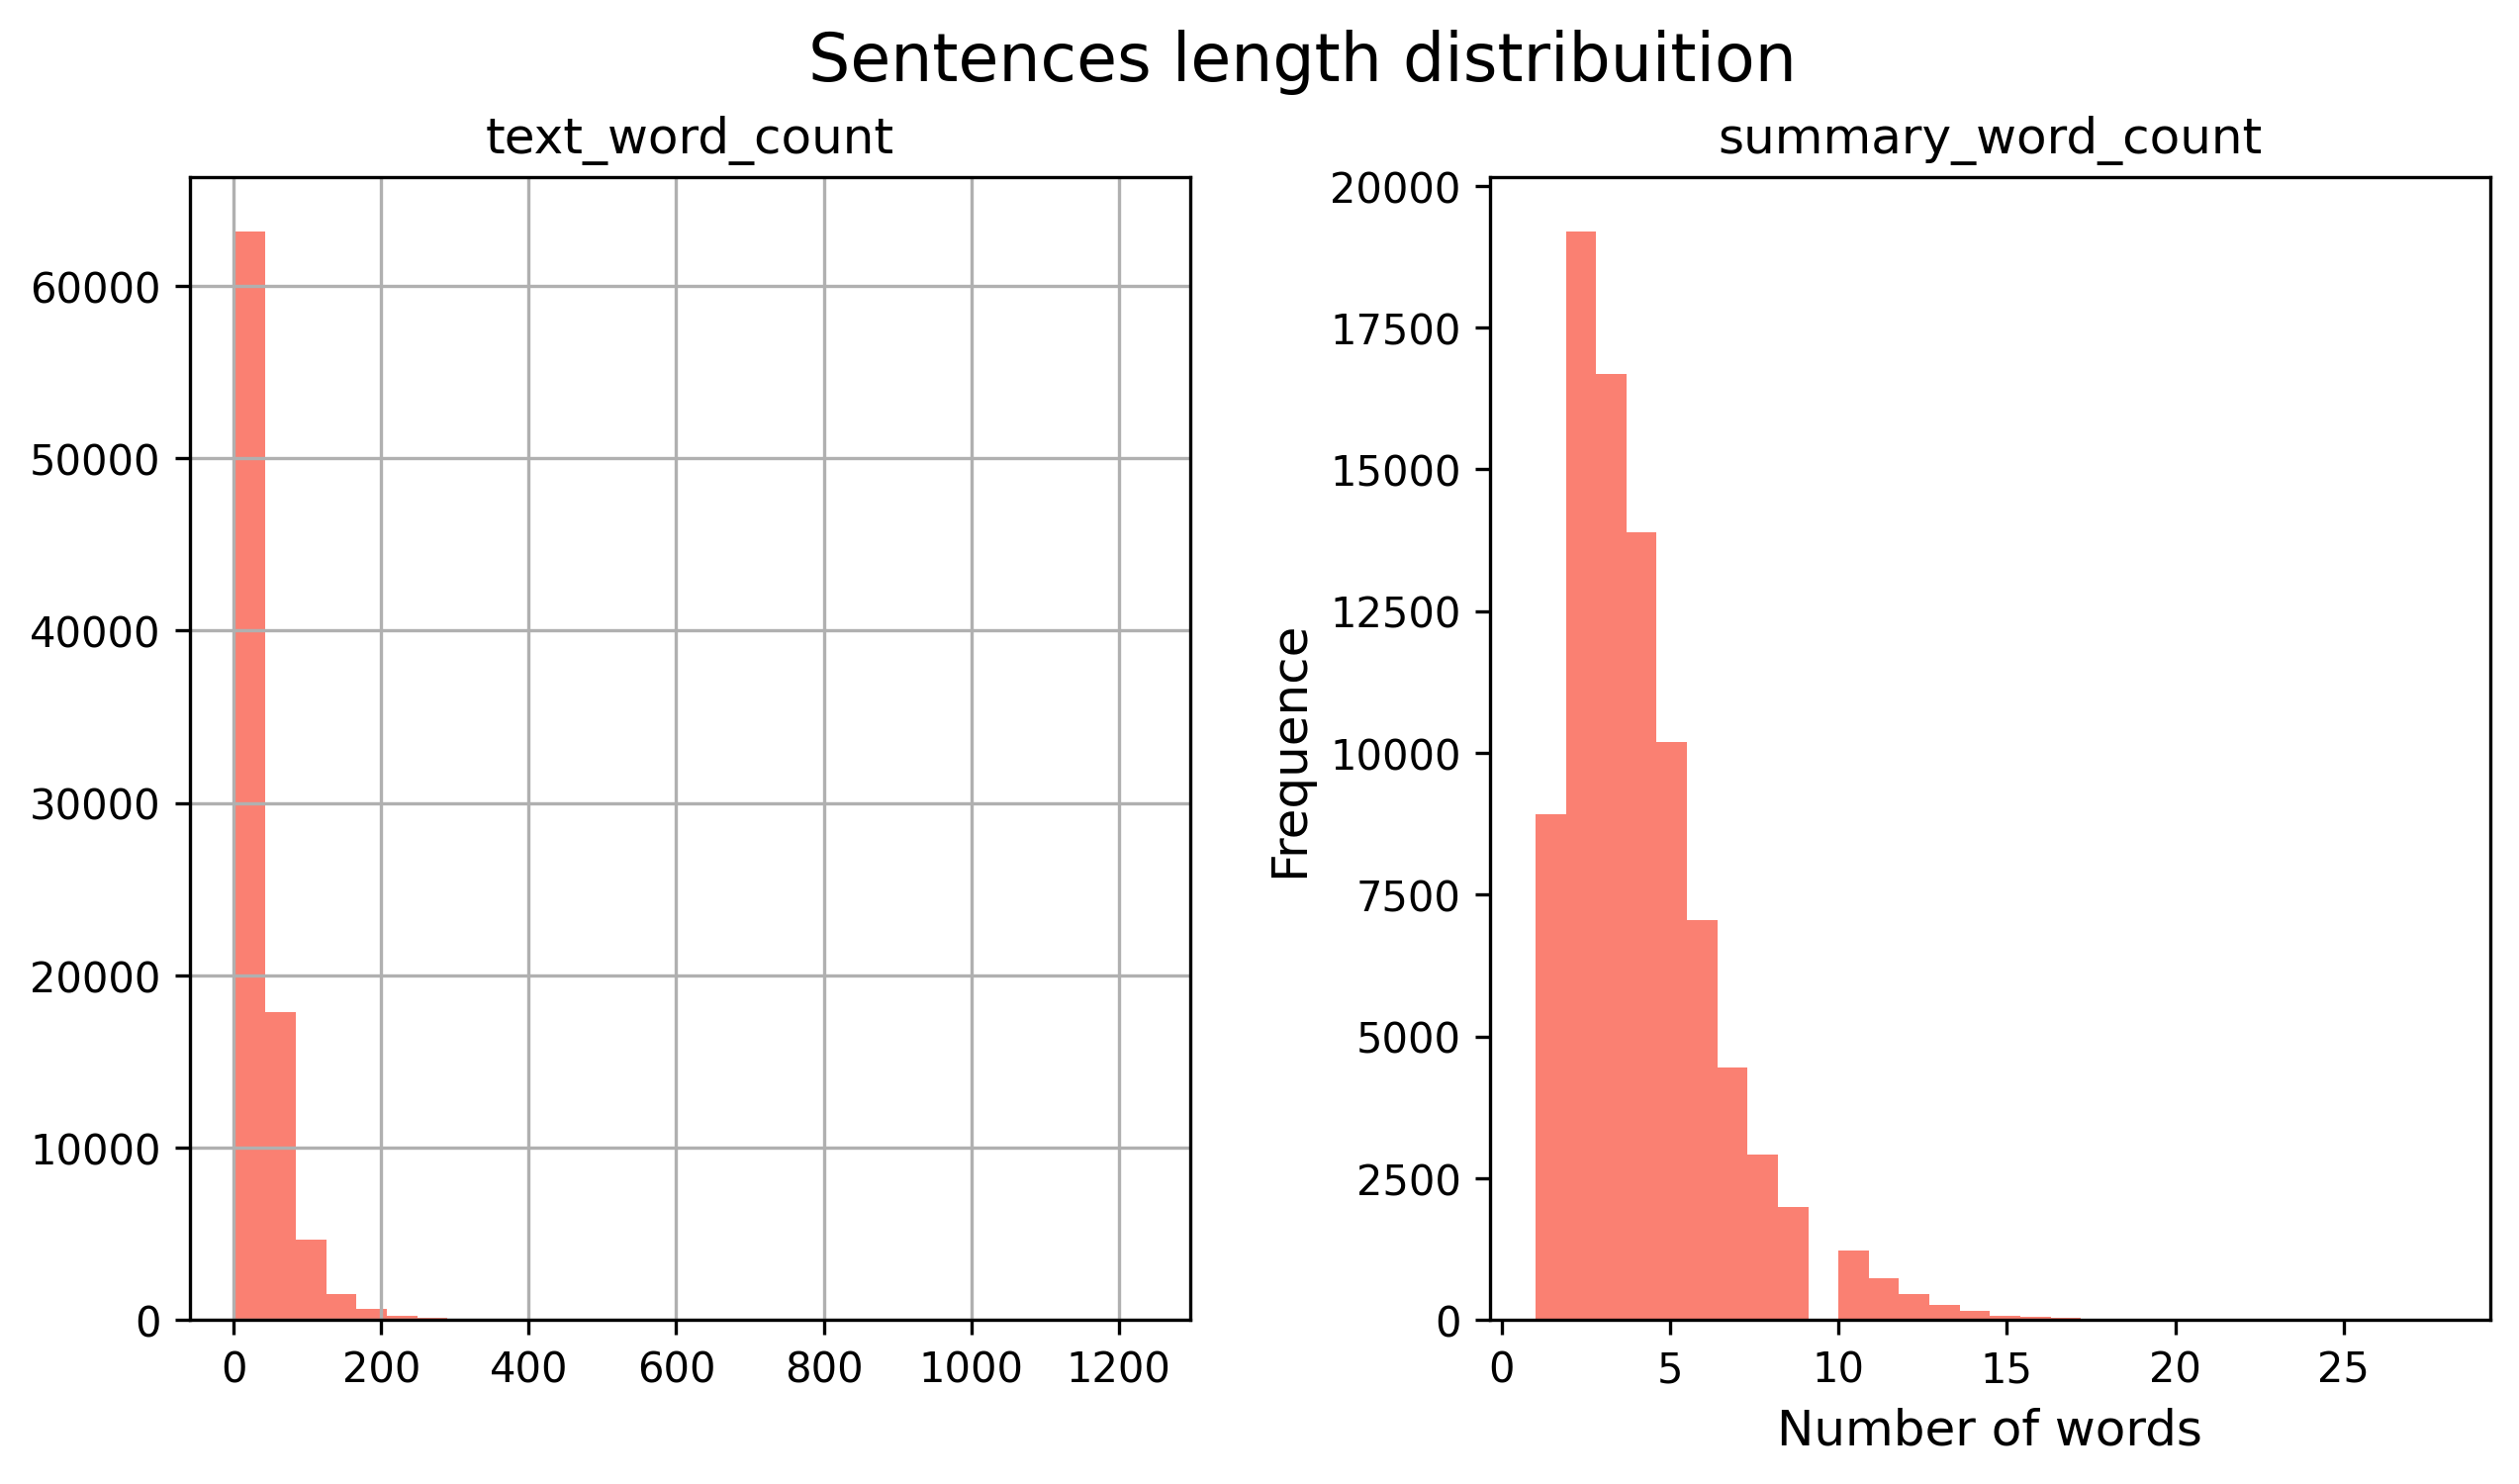
\includegraphics[width=1\textwidth]{media/dataset_length_distribuition.png}
    \caption{A sinistra la distribuzione delle lunghezze delle recensioni, a destra la distribuzione delle lunghezze dei riassunti}
    \label{fig:dataset_length_distribuition}
\end{figure}
Infatti, come si puè notare dai due grafici, la maggior parte delle recensioni e dei riassunti ha lunghezze inferiori ai limiti stabiliti, quindi questi vincoli permettono di mantenere la maggior parte dei dati del dataset.

\subsection{Tokenizzazione e Token Speciali}
Per preparare i dati per il modello ho aggiunto i token speciali \texttt{"sostok"} e \texttt{"eostok"} per indicare l'inizio e la fine di una sequenza, in modo da facilitare la tokenizzazione e l'addestramento del modello.\\
Inoltre, ho effettuato la tokenizzazione separata per le recensioni (testo di input) e i riassunti (testo di output) per garantire che il modello possa apprendere correttamente la relazione tra i due.
I due tokenizer servono a creare il vocabolario per le recensioni e per i riassunti, in modo da poter convertire i testi in sequenze di token.

\section{Architettura del Modello}
L'implementazione del modello è stata effettuata attraverso una classe astratta \texttt{BaseModel} e una classe derivata \texttt{   LSTM}.\\
Questo permette di definire un'interfaccia comune per tutti i modelli di summarization e di estendere facilmente l'architettura in futuro.\\

\subsection{Classe Base Astratta}
La classe \texttt{BaseModel} fornisce l'interfaccia base per tutti i modelli di summarization:
\begin{itemize}
    \item Metodi astratti per costruire encoder e decoder.
    \item Funzionalità per il salvataggio, caricamento e inferenza del modello.
    \item Conversione tra sequenze e testo tramite i tokenizzatori.
\end{itemize}

\subsection{Implementazione Seq2SeqLSTM}
La classe \texttt{Seq2SeqLSTM} implementa l'architettura specifica per il modello di summarization Sequence to Sequence con layer LSTM.\\
Vediamo di seguito le caratteristiche principali dell'architettura, composta da encoder e decoder:

\subsubsection{Encoder}
L'encoder è composto da:
\begin{itemize}
    \item \textbf{Layer di embedding}: mappa i token di input in vettori di lunghezza fissa
    \item \textbf{Tre layer LSTM} con:
        \begin{itemize}
            \item Dimensione latente fissa
            \item Dropout del 40\% 
            \item Recurrent dropout del 20\% 
        \end{itemize}
\end{itemize}

\subsubsection{Decoder}
Il decoder include:
\begin{itemize}
    \item \textbf{Layer di embedding}: mappa i token di output in vettori di lunghezza fissa
    \item \textbf{Layer LSTM} con:
        \begin{itemize}
            \item Stessa dimensione latente dell'encoder
            \item Dropout del 40\%
            \item Recurrent dropout del 20\%
        \end{itemize}
    \item \textbf{Layer di attention}: calcola i pesi di attenzione tra l'encoder e il decoder
    \item \textbf{Layer denso di output}: questo layer restituisce la distribuzione di probabilità sul vocabolario per la generazione delle parole del riassunto.\\ 
    Utilizza la funzione di attivazione softmax per la normalizzazione delle probabilità.
\end{itemize}

Di seguito, nella figura \ref{fig:model_architecture}, possiamo vedere un diagramma dell'architettura del modello:
\begin{figure}[H]
    \centering
    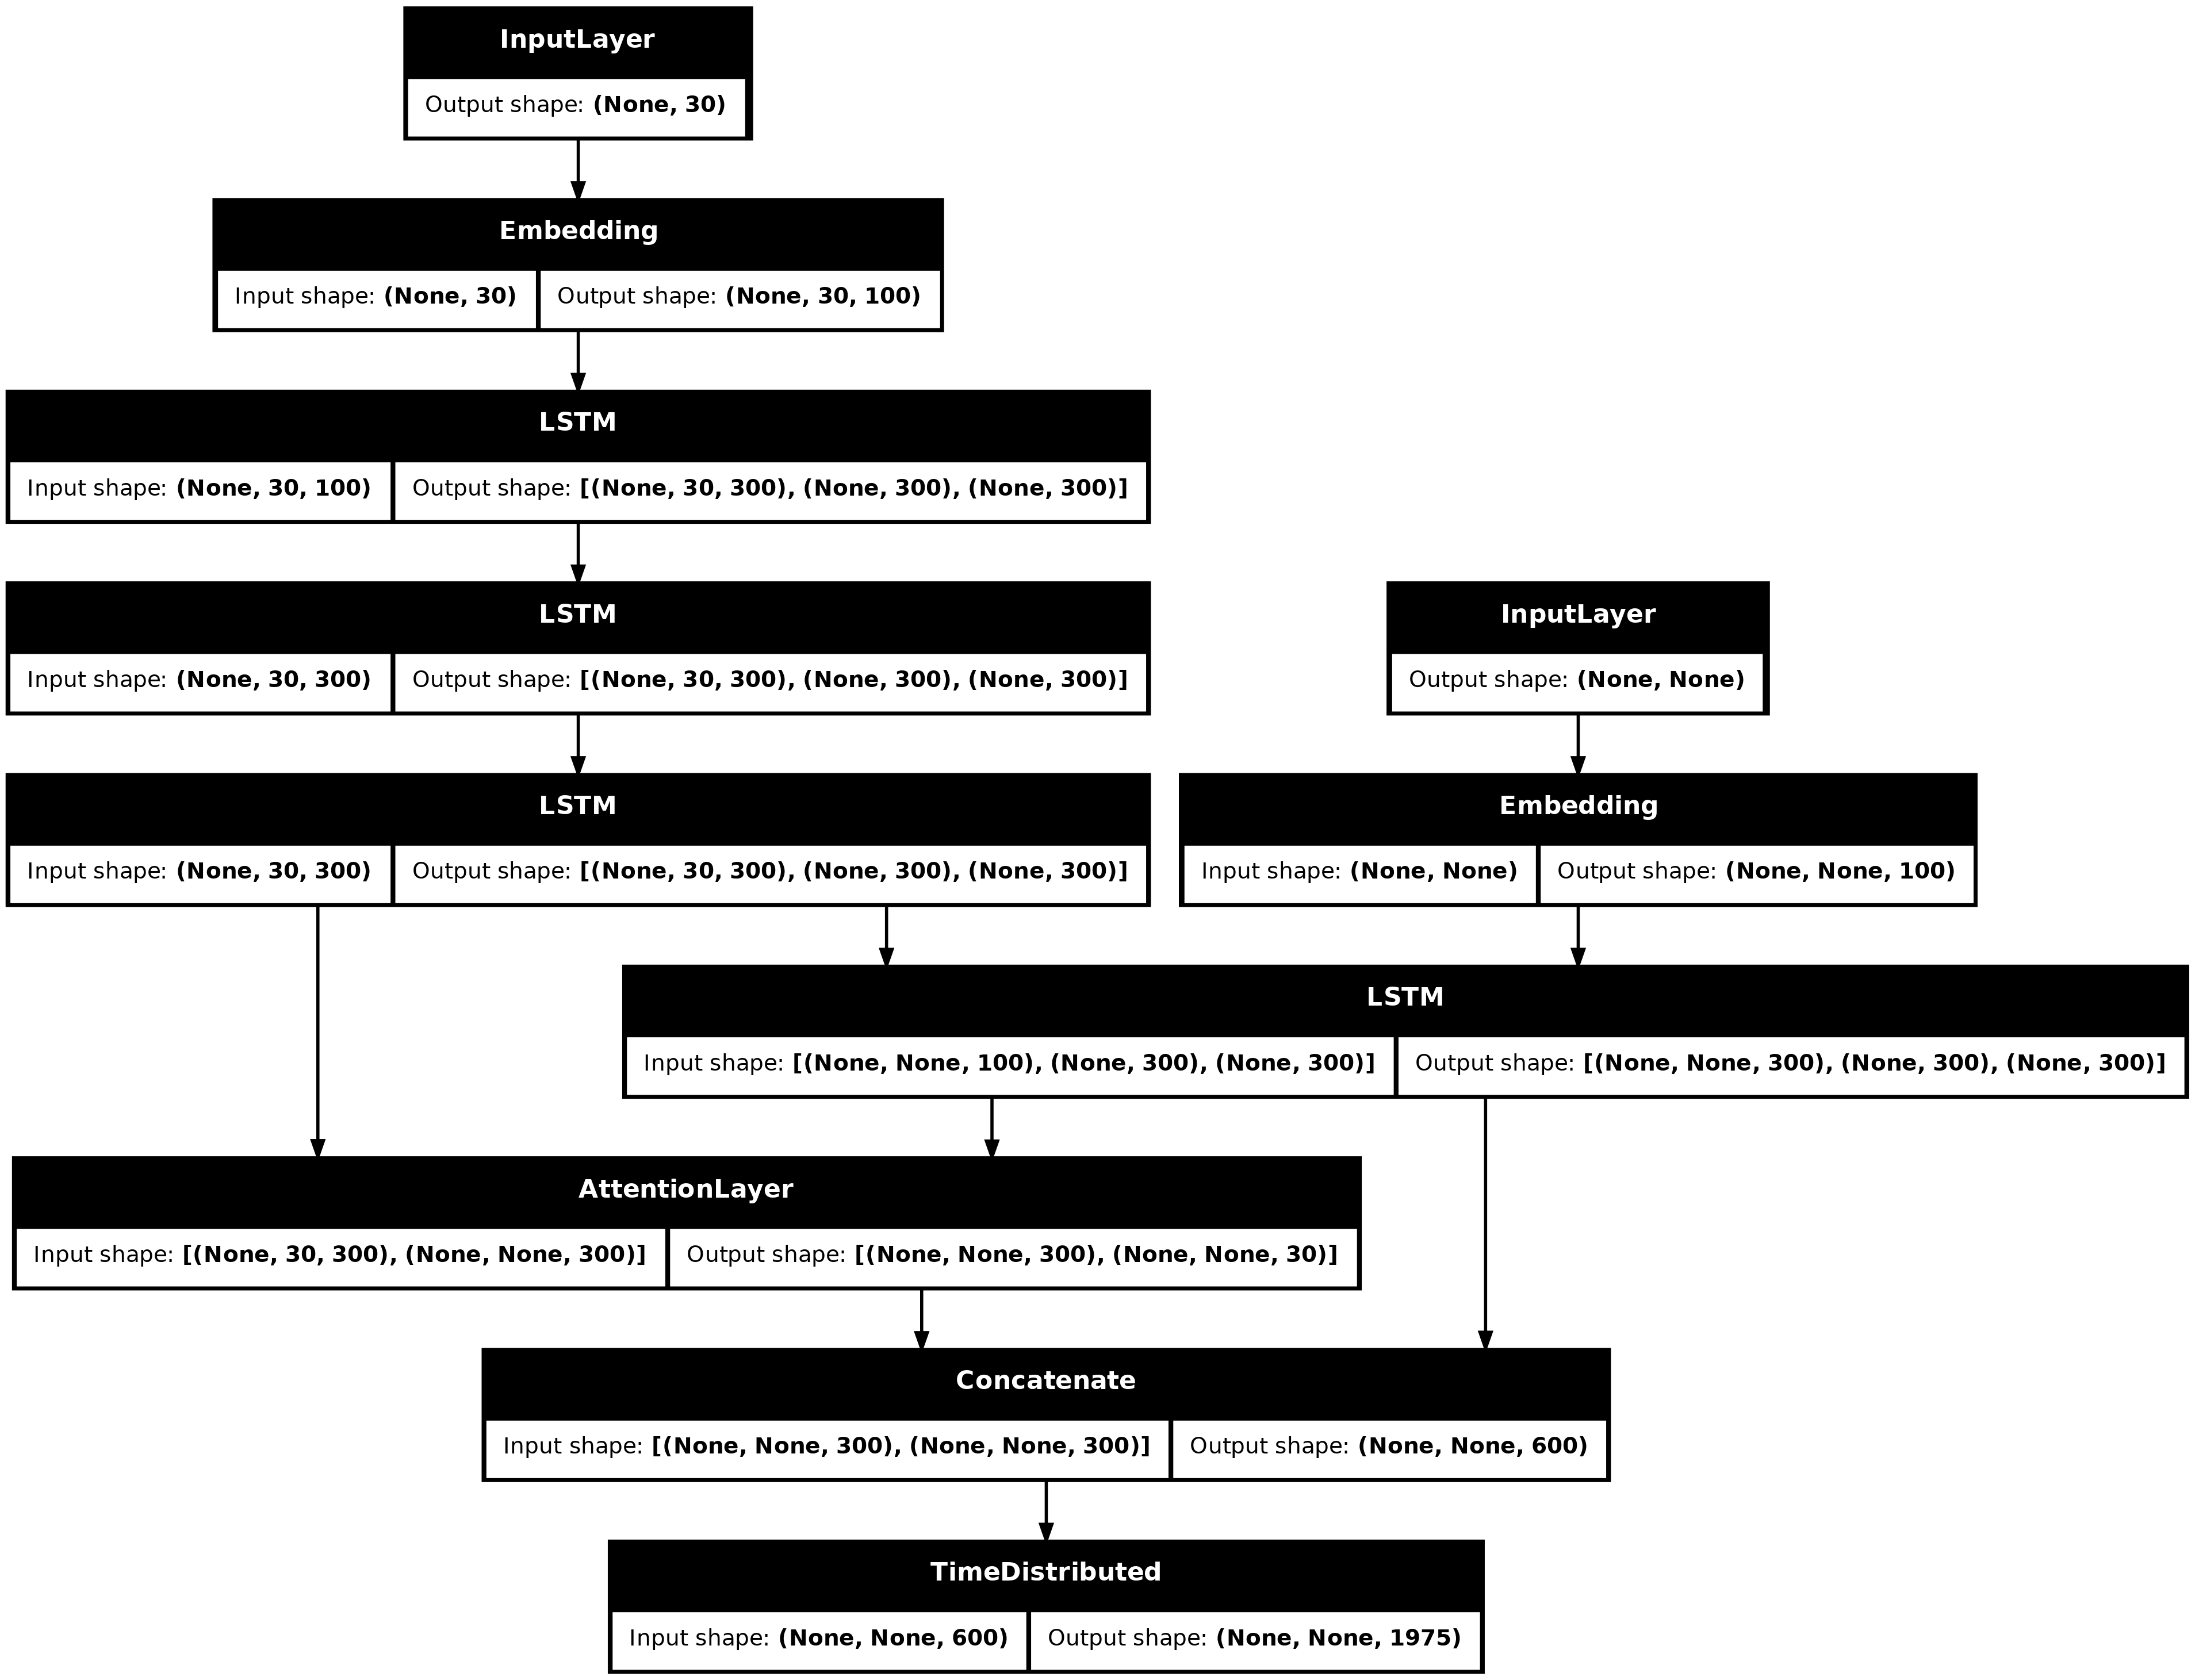
\includegraphics[width=1\textwidth]{media/Seq2SeqLSTM_originale_image.png}
    \caption{Diagramma dell'architettura del modello}
    \label{fig:model_architecture}
\end{figure}

\section{Training del Modello}
L'addestramento del modello è stato effettuato utilizzando il dataset preprocessato.\\
Prima di iniziare l'addestramento, il dataset è stato suddiviso in training set e validation set, con una proporzione del 90\% e 10\% rispettivamente.\\
A questo punto ho definito una funzione di early stopping per monitorare la loss sul validation set e fermare l'addestramento quando la loss non diminuisce per un certo numero di epoche, ciò per evitare l'overfitting.\\
Dopodiché sono passato alla fase effettiva di training del modello, utilizzando l'ottimizzatore \texttt{rmsprop} e la loss function \texttt{categorical crossentropy}.\\

\subsection{Loss}
Alla fine dell'addestramento, la loss sul training set è scesa a circa , mentre la loss sul validation set è arrivata a .\\
Possiamo verifcare l'andamento delle loss durante l'addestramento nella figura \ref{fig:loss_plot}.
\begin{figure}[H]
    \centering
    %TODO: Aggiungere immagine traingin loss
    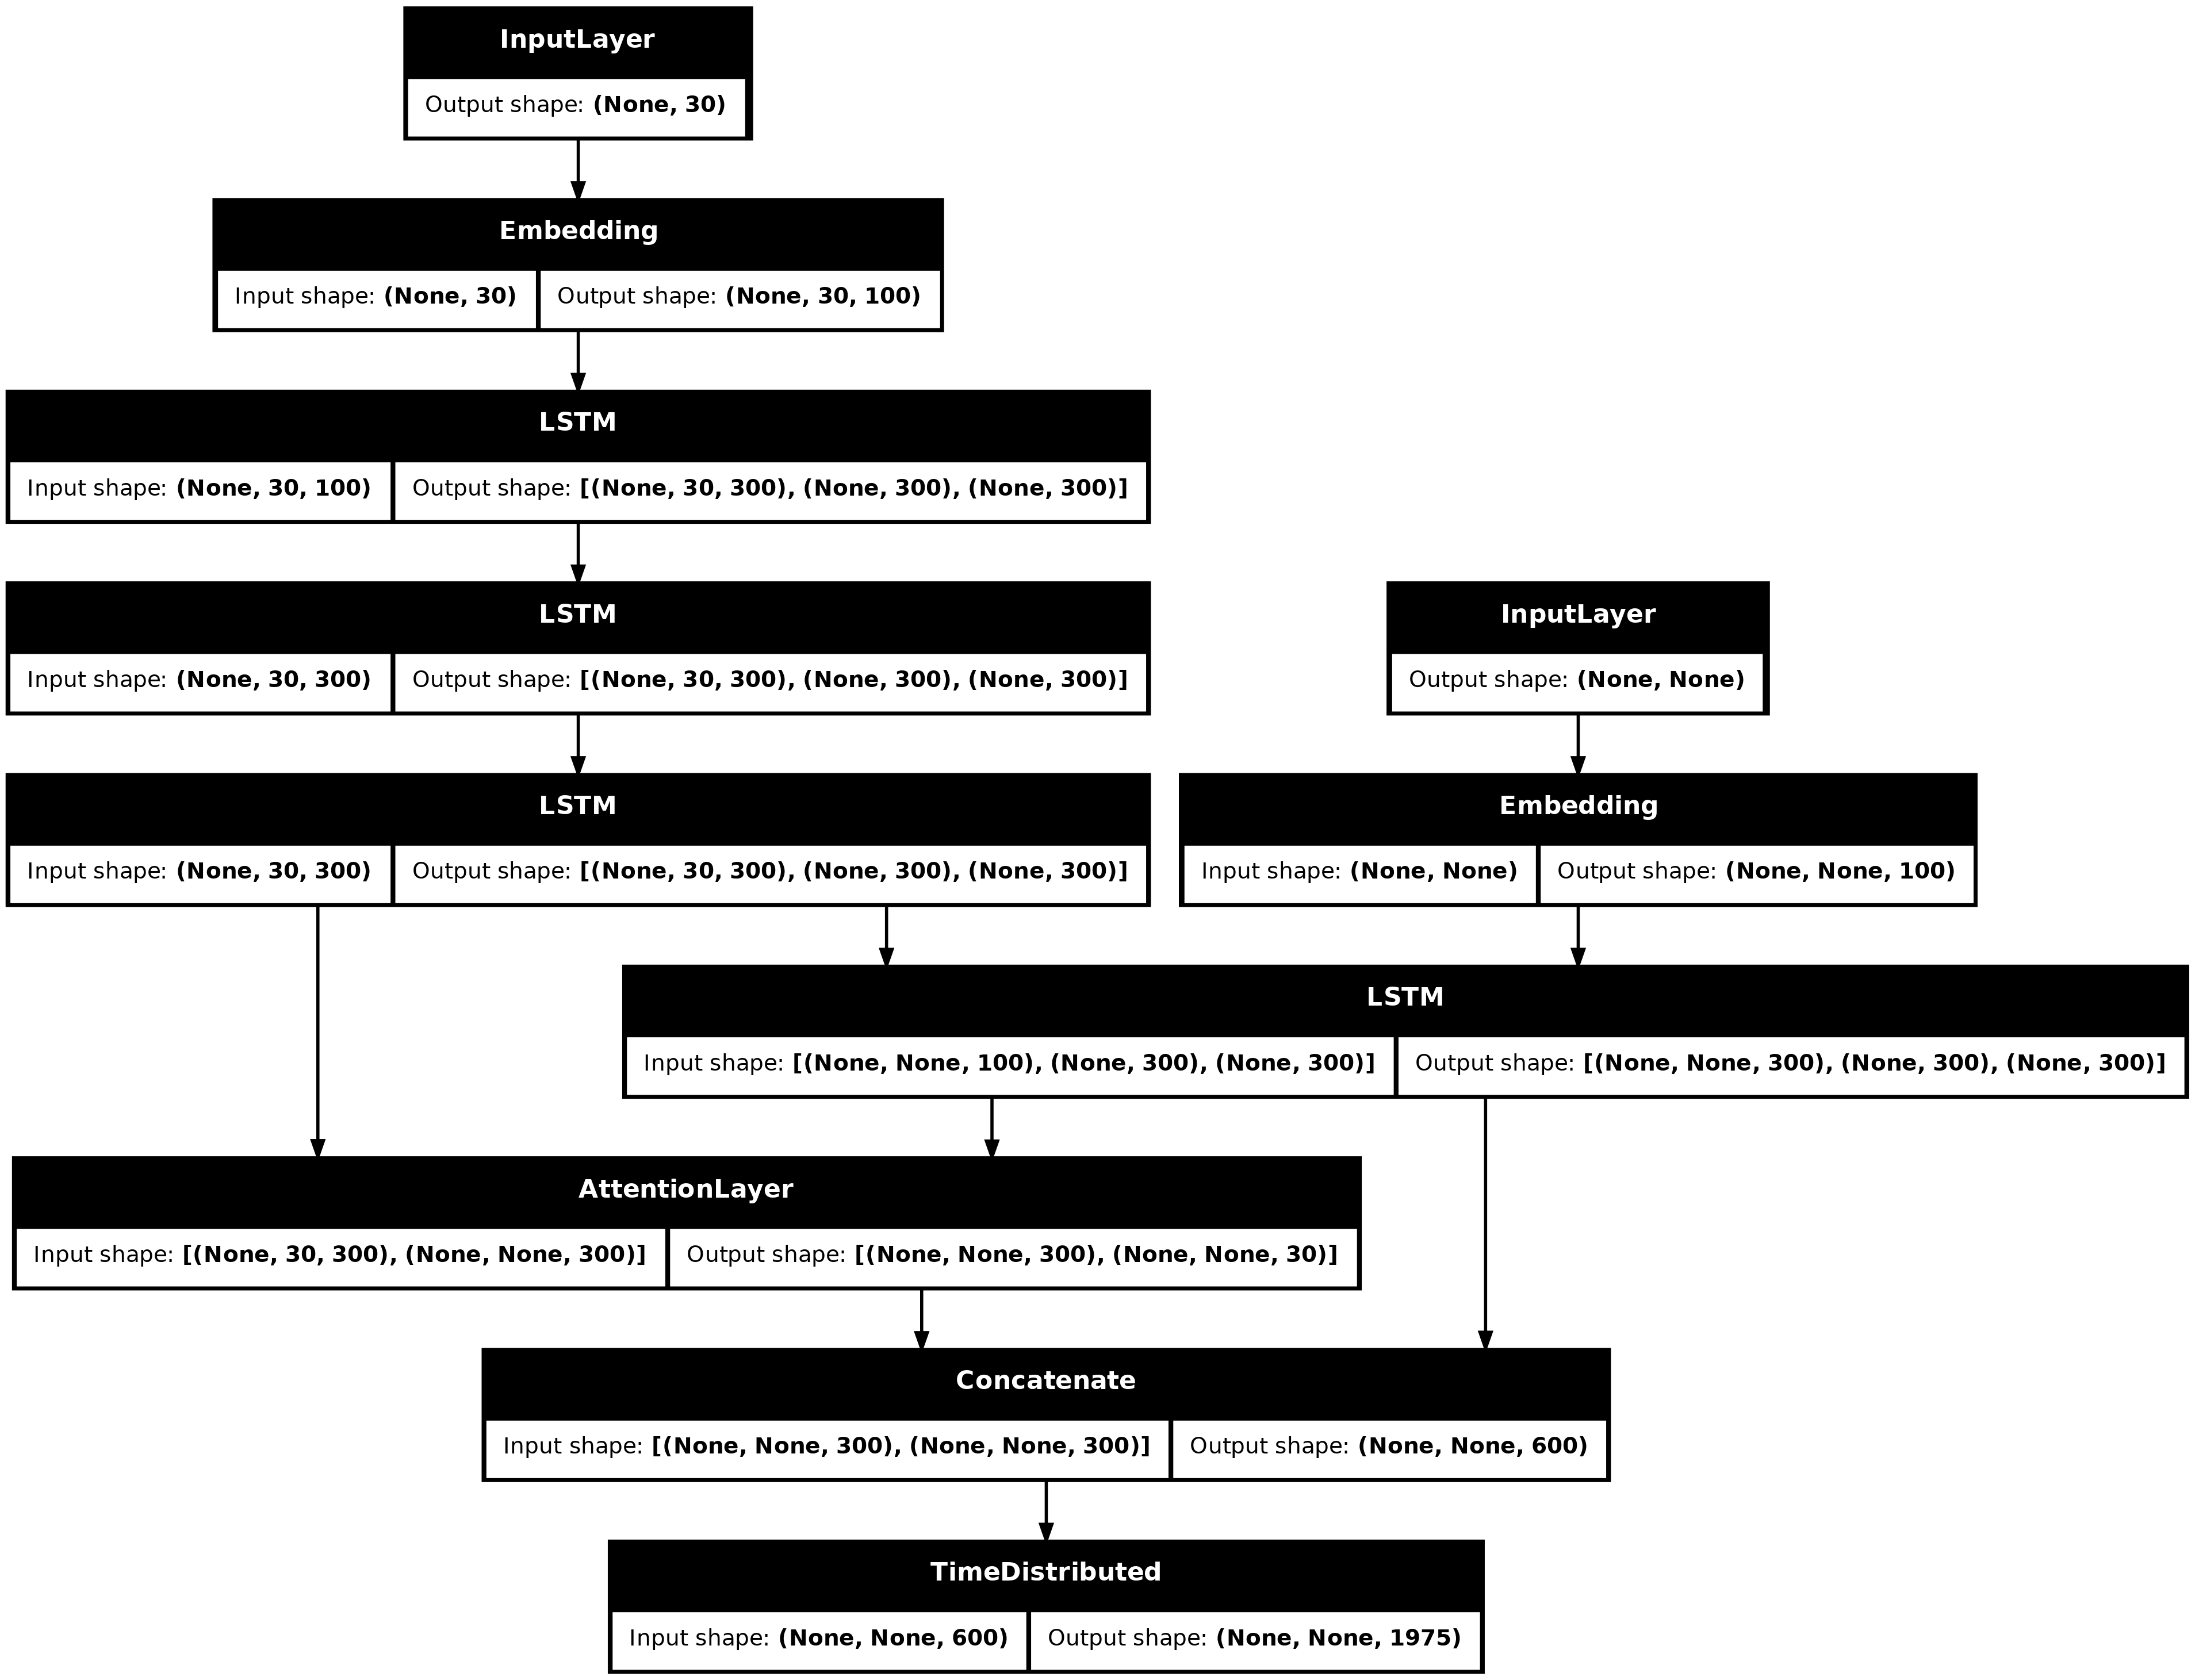
\includegraphics[width=1\textwidth]{media/Seq2SeqLSTM_originale_image.png}
    \caption{Andamento delle loss durante l'addestramento}
    \label{fig:loss_plot}
\end{figure}

\section{Metriche di Valutazione}
Per valutare le performance del modello sono state utilizzate diverse metriche, utili per valutare la qualità dei riassunti generati rispetto a quelli di riferimento.\\
Per eseguire queste valutazioni ho utilizzato il dataset di test, che non è stato utilizzato durante l'addestramento del modello e ho fatto inferenza sui dati di test per generare i riassunti, per la precisione ho generato 1000 riassunti.\\

\subsection{ROUGE (Recall-Oriented Understudy for Gisting Evaluation)}
Sono state calcolate tre varianti di ROUGE:
\begin{itemize}
    \item ROUGE-1: confronta unigrammi tra il riassunto generato e quello di riferimento, \ref{fig:rouge_1}
    \item ROUGE-2: considera bigrammi per valutare la similarità tra i due testi, \ref{fig:rouge_2}
    \item ROUGE-L: confronta la sottosequenza più lunga comune tra i due testi, \ref{fig:rouge_l}
\end{itemize}

\begin{figure}[H]
    \centering
    \begin{subfigure}{0.32\textwidth}
        \centering
        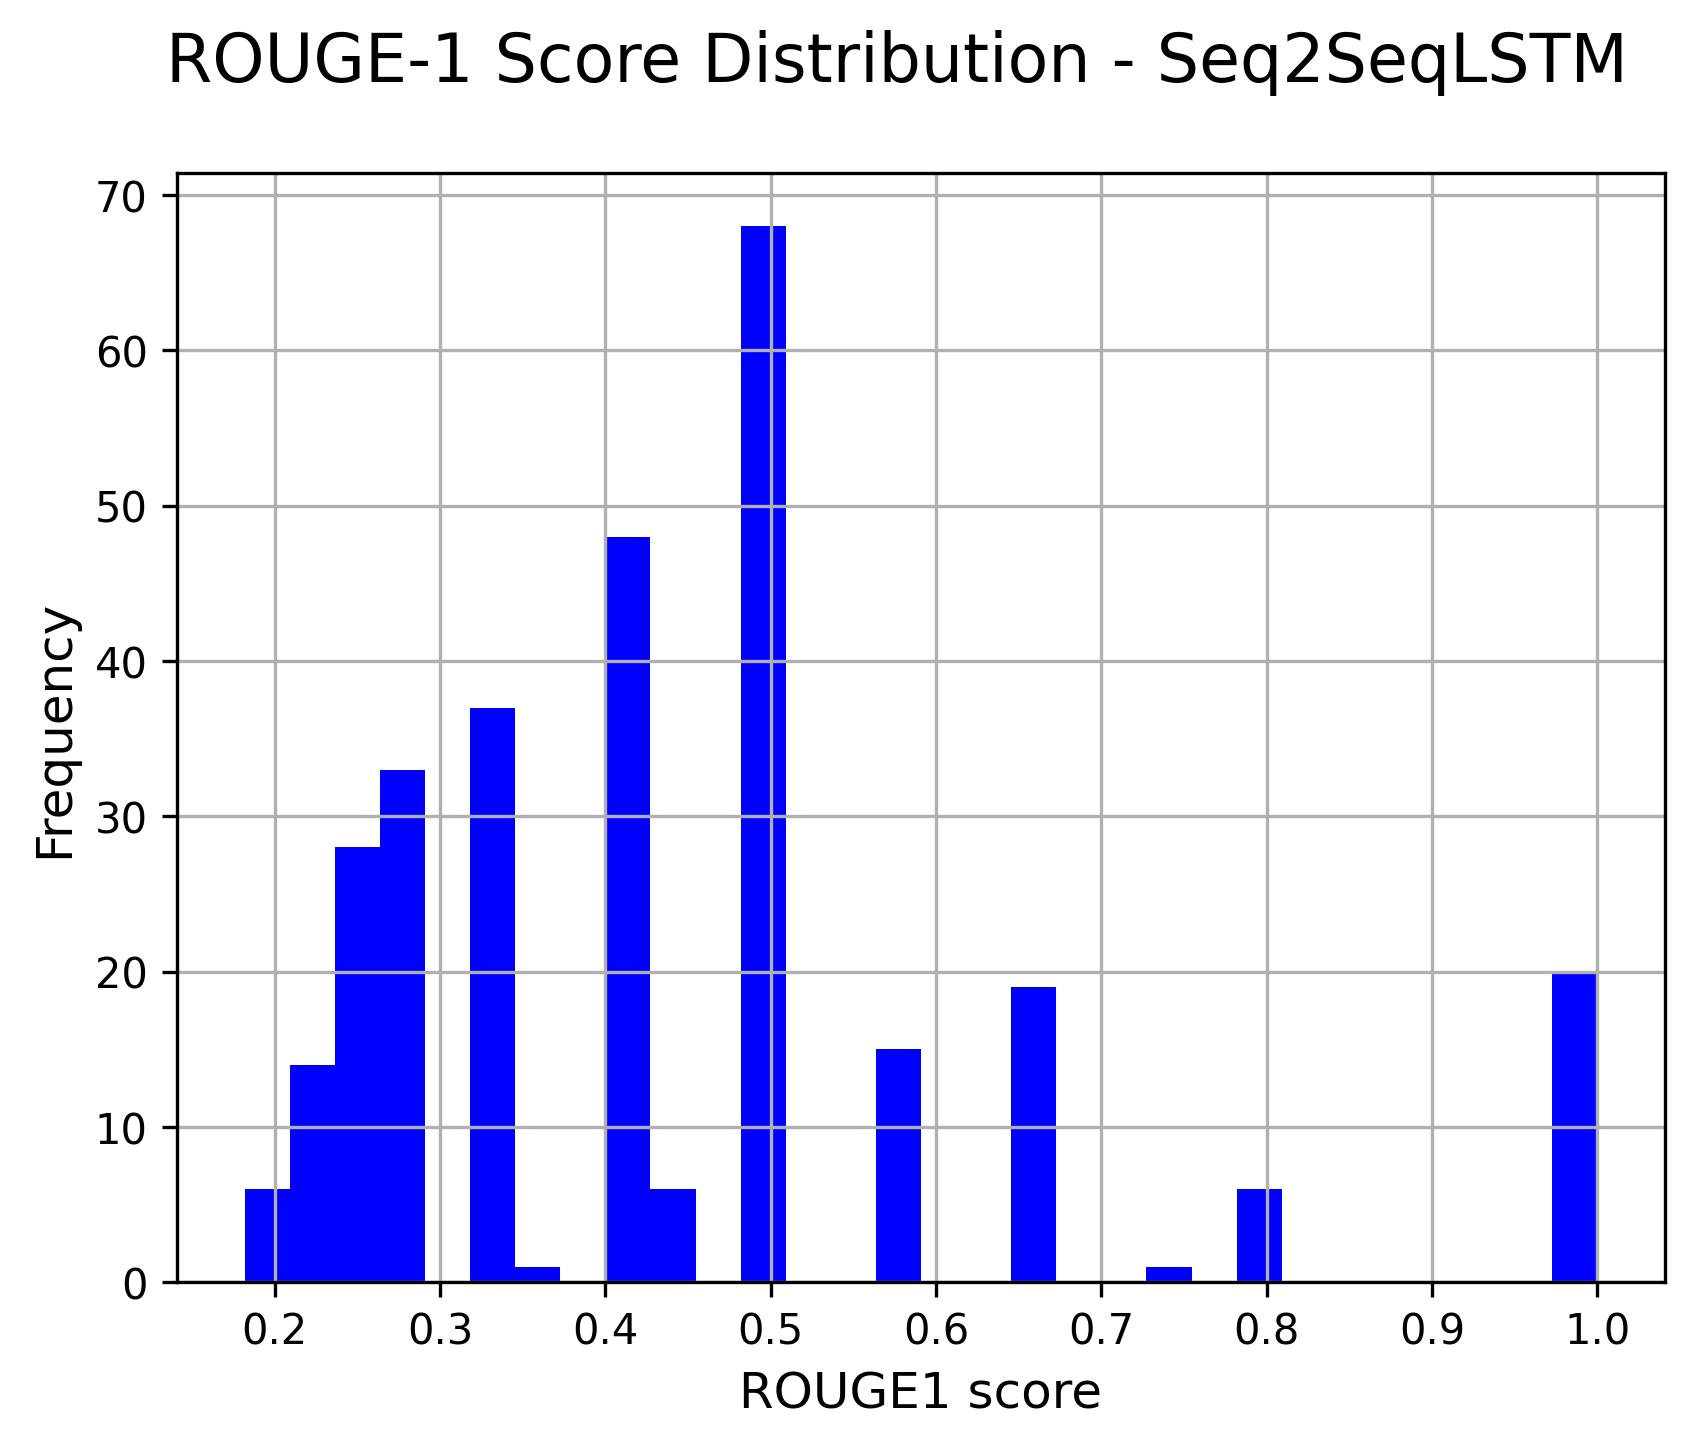
\includegraphics[width=\textwidth]{media/Seq2SeqLSTM_rouge1_scores.png}
        \caption{ROUGE-1}
        \label{fig:rouge_1}
    \end{subfigure}
    \hfill
    \begin{subfigure}{0.32\textwidth}
        \centering
        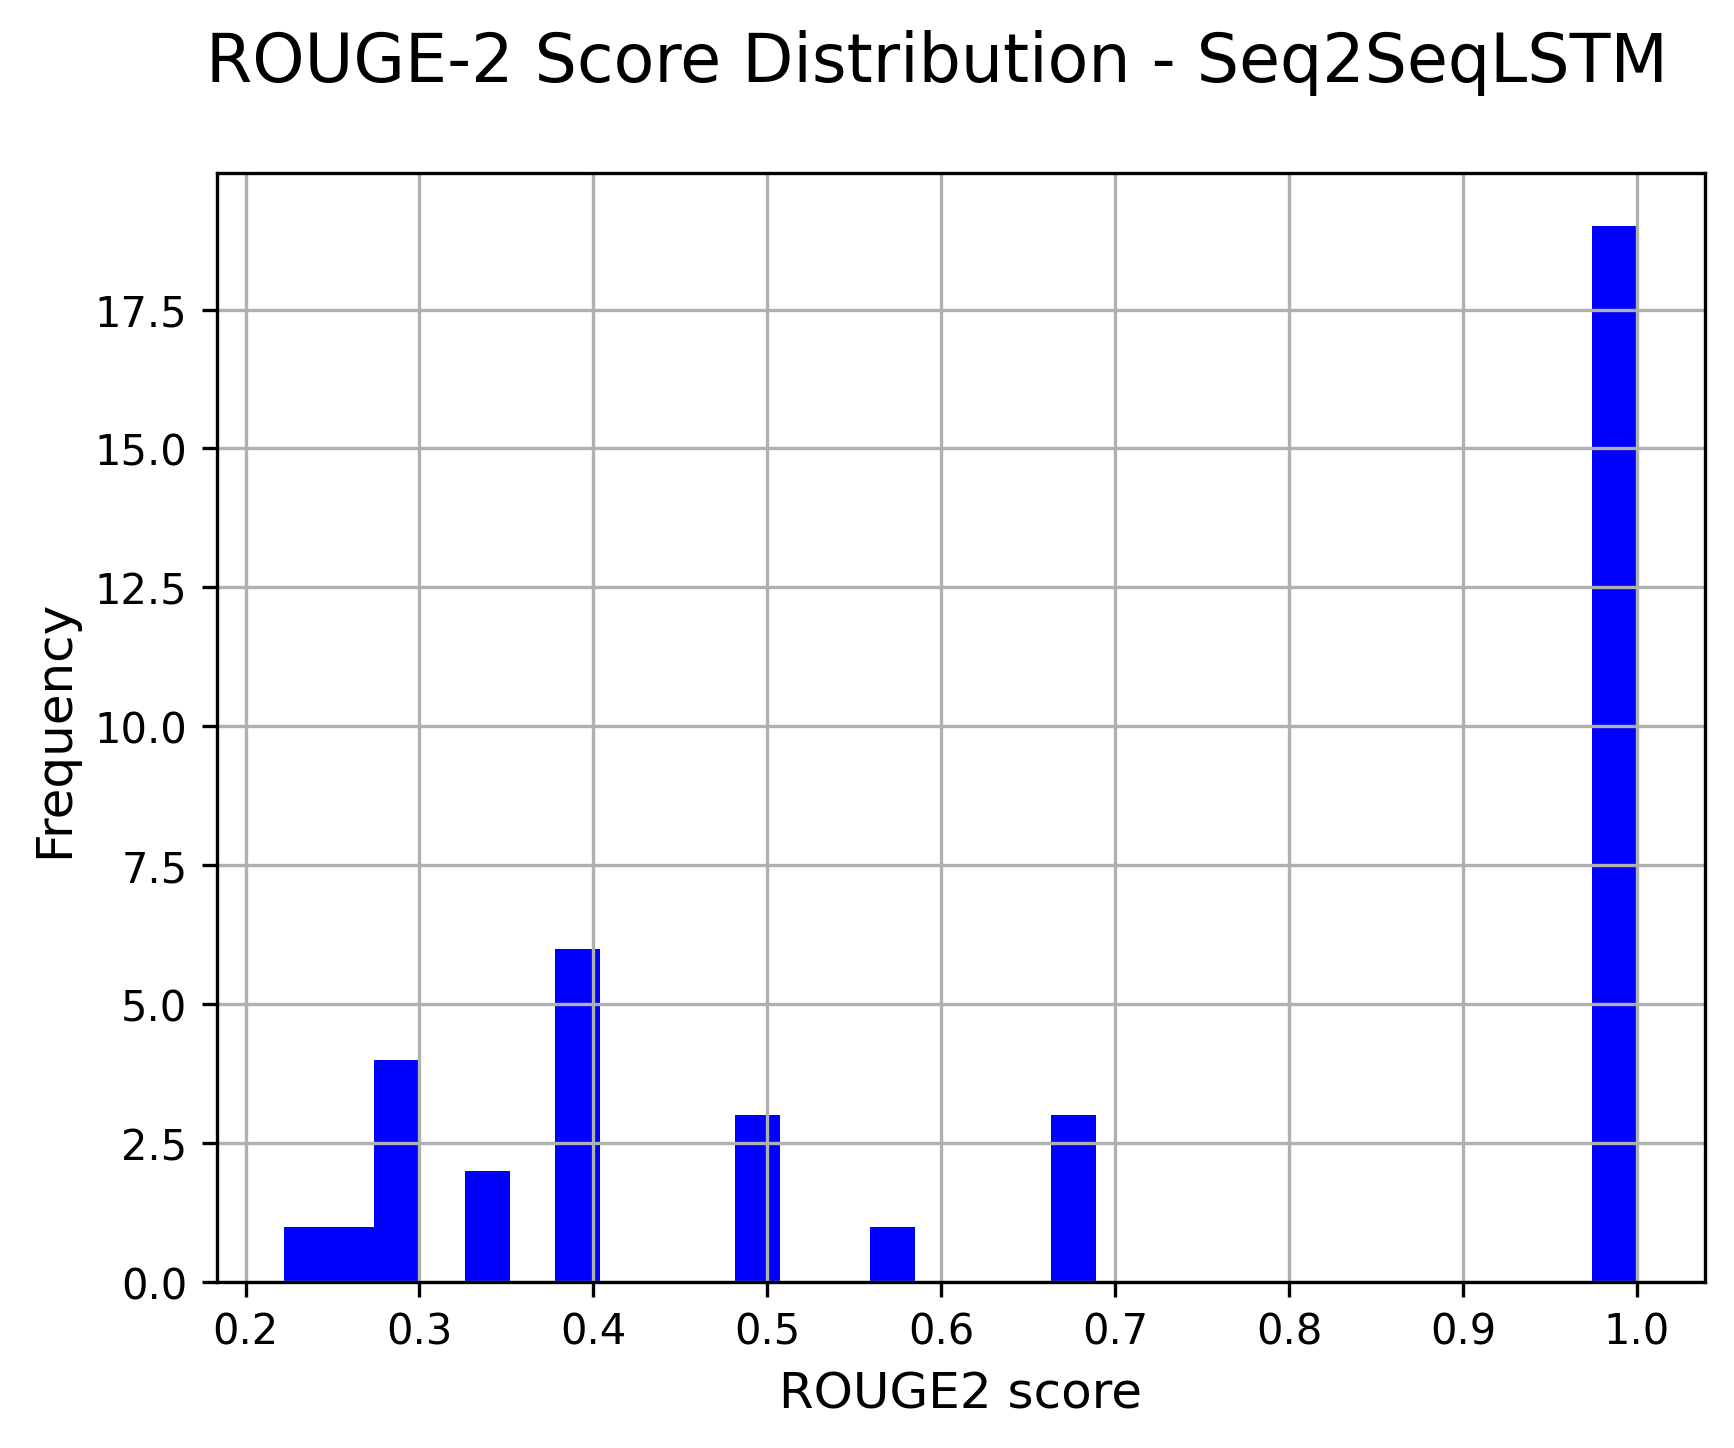
\includegraphics[width=\textwidth]{media/Seq2SeqLSTM_rouge2_scores.png}
        \caption{ROUGE-2}
        \label{fig:rouge_2}
    \end{subfigure}
    \hfill
    \begin{subfigure}{0.32\textwidth}
        \centering
        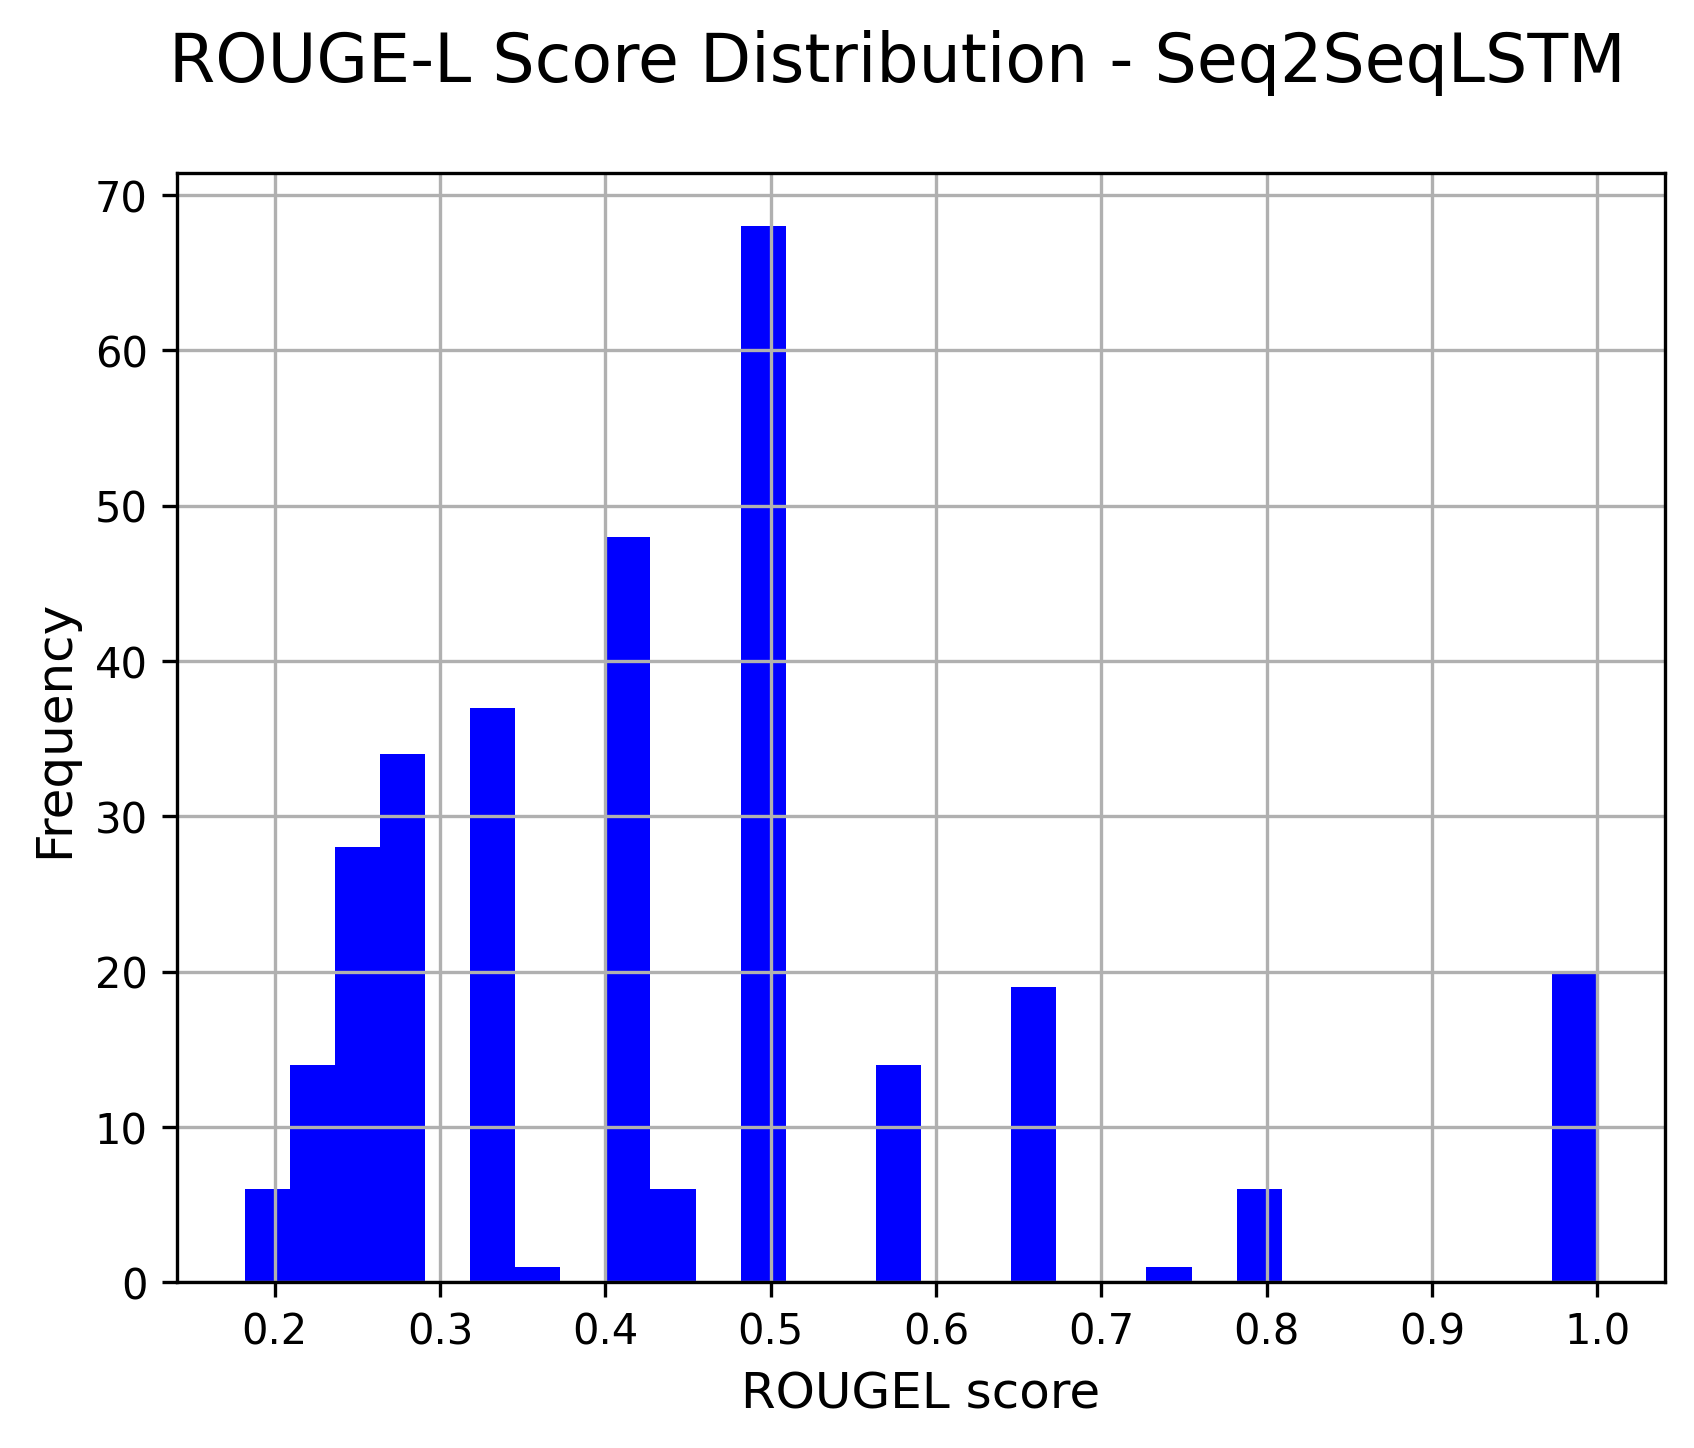
\includegraphics[width=\textwidth]{media/Seq2SeqLSTM_rougeL_scores.png}
        \caption{ROUGE-L}
        \label{fig:rouge_l}
    \end{subfigure}
    \caption{Valori ROUGE per il modello Seq2SeqLSTM: (a) ROUGE-1, (b) ROUGE-2, and (c) ROUGE-L.}
    \label{fig:rouge_scores}
\end{figure}


\subsection{Word Error Rate (WER)}
Il WER è una metrica che calcola il tasso di errore tra due sequenze di parole.\\
In particolare, il WER calcola il numero di operazioni di inserimento, cancellazione e sostituzione necessarie per trasformare una sequenza di parole in un'altra.\\
\begin{figure}[H]
    \centering
    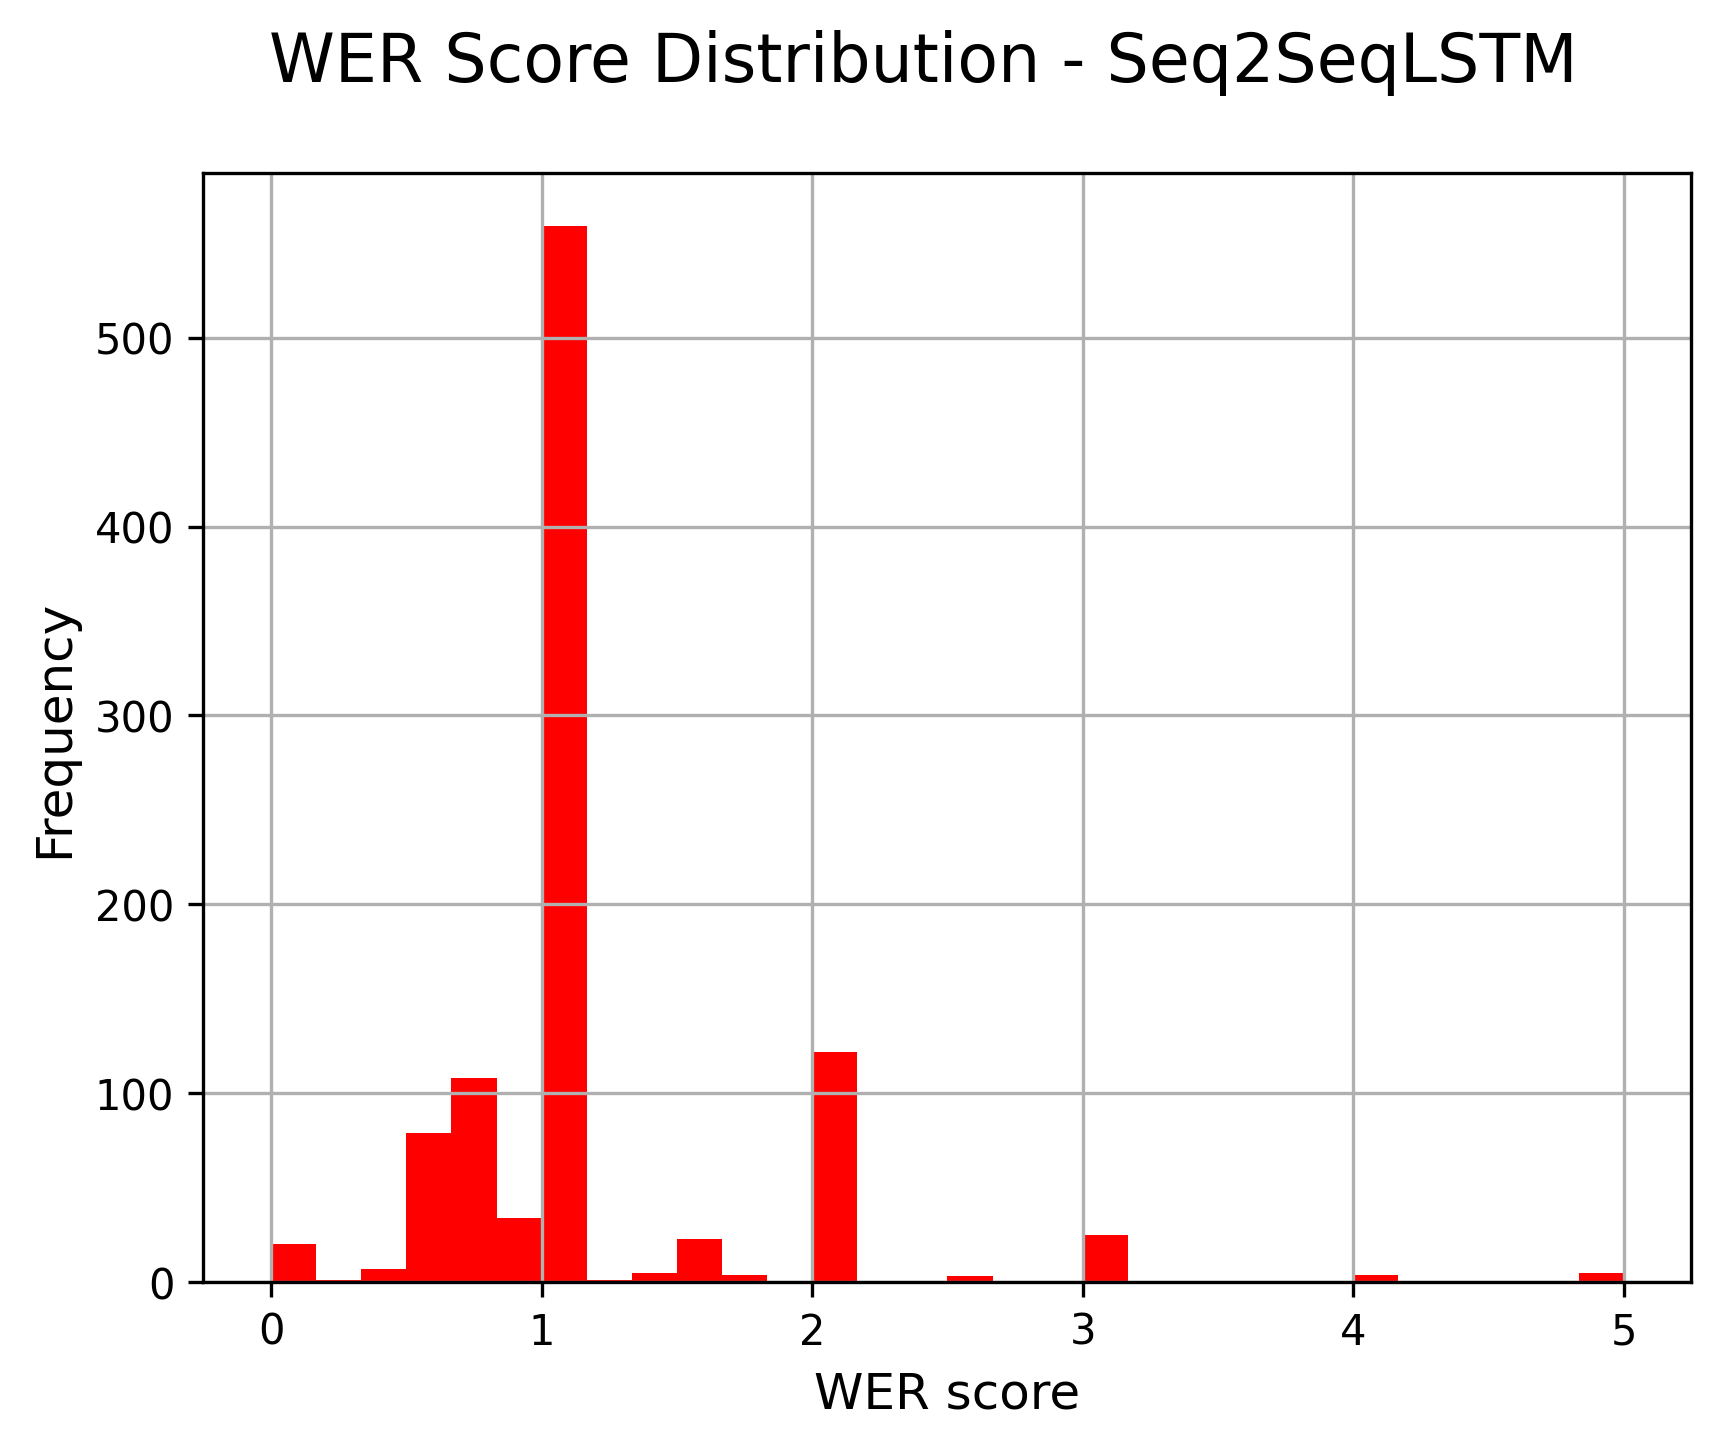
\includegraphics[width=0.75\textwidth]{media/Seq2SeqLSTM_wer_scores.png}
    \caption{Valori WER per il modello Seq2SeqLSTM}
    \label{fig:wer}
\end{figure}


\subsection{Cosine Similarity}
La similarità cosenica è una metrica che calcola la similarità tra due vettori in uno spazio multidimensionale.\\
Nel caso specifico della generazione di riassunti, la similarità cosenica è stata calcolata tra i vettori di embedding delle parole nei riassunti generati e quelli nei riassunti di riferimento, con il fine di valutare la qualità dei riassunti generati.\\
\begin{figure}[H]
    \centering
    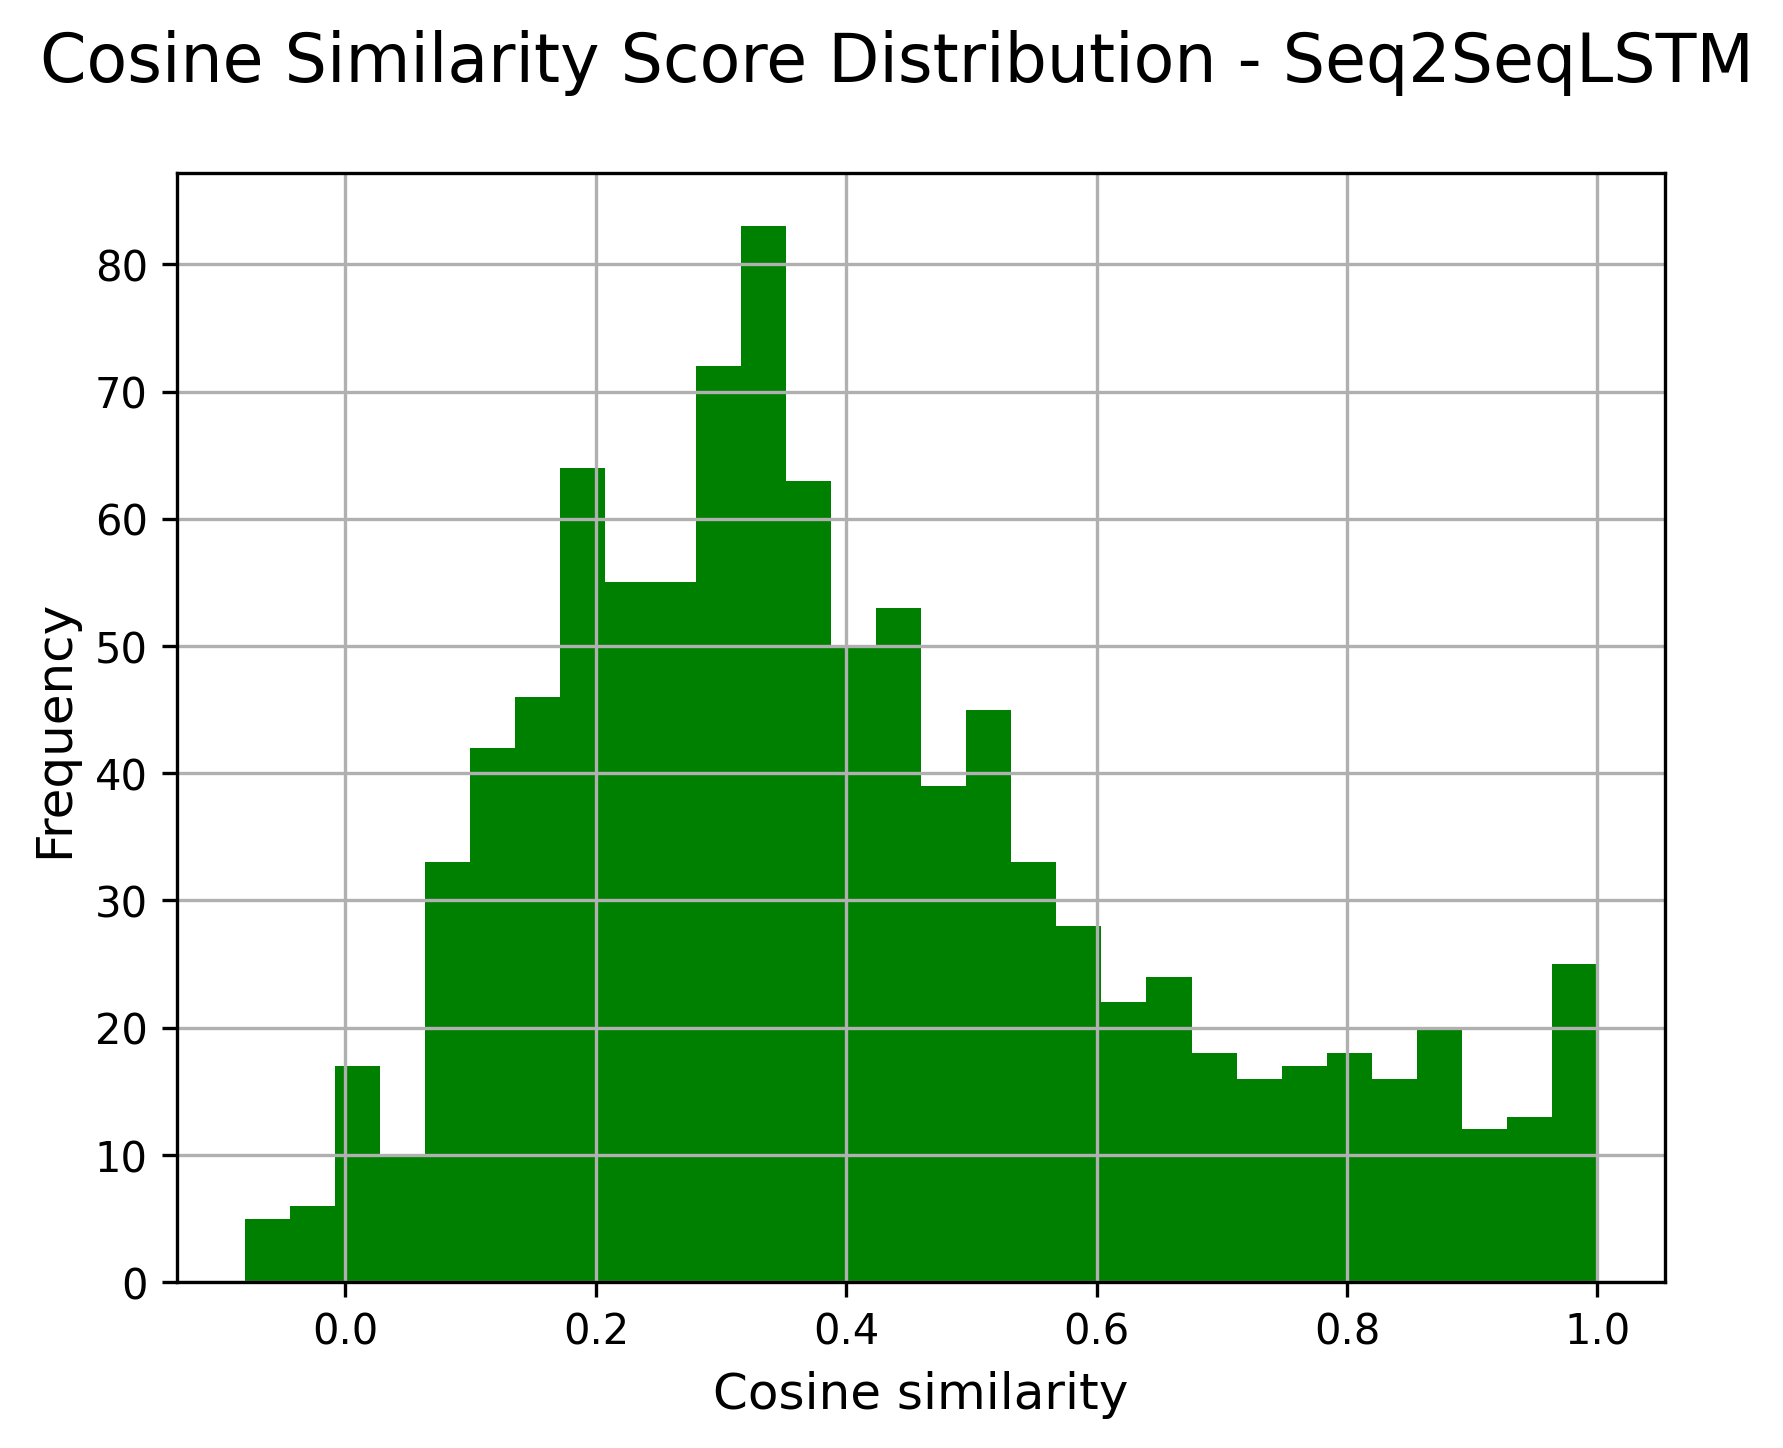
\includegraphics[width=0.75\textwidth]{media/Seq2SeqLSTM_cosine_similarity_scores.png}
    \caption{Valori di similarità cosenica per il modello Seq2SeqLSTM}
    \label{fig:cosine_similarity}
\end{figure}

\section{Implementazione del Modello Seq2SeqBiLSTM}

In questo caso, abbiamo implementato un modello di tipo Sequence-to-Sequence con una versione BiLSTM (Bidirectional LSTM).\\
L'architettura è simile al modello Seq2Seq LSTM, ma con un'encoder bidirezionale, il che consente di catturare informazioni contestuali da entrambe le direzioni della sequenza.

\subsection{Architettura del Modello Seq2SeqBiLSTM}
L'architettura del modello Seq2SeqBiLSTM include le seguenti modifiche rispetto al modello LSTM standard:

\subsubsection{Encoder}
L'encoder è composto da:
\begin{itemize}
    \item \textbf{Layer di embedding}: mappa i token di input in vettori di lunghezza fissa.
    \item \textbf{Due layer LSTM bidirezionali} con:
        \begin{itemize}
            \item Dimensione latente fissa.
            \item Dropout del 40\%.
            \item Recurrent dropout del 20\%.
        \end{itemize}
\end{itemize}

\subsubsection{Decoder}
Il decoder include:
\begin{itemize}
    \item \textbf{Layer di embedding}: mappa i token di output in vettori di lunghezza fissa.
    \item \textbf{Layer LSTM}: stessa dimensione latente dell'encoder.
    \item \textbf{Layer di attenzione}: calcola i pesi di attenzione tra l'encoder e il decoder.
    \item \textbf{Layer denso di output}: restituisce la distribuzione di probabilità per la generazione delle parole del riassunto.
\end{itemize}

Di seguito, possiamo vedere un diagramma dell'architettura del modello Seq2SeqBiLSTM nella figura \ref{fig:biLSTM_model_architecture}.

\begin{figure}[H]
    \centering
    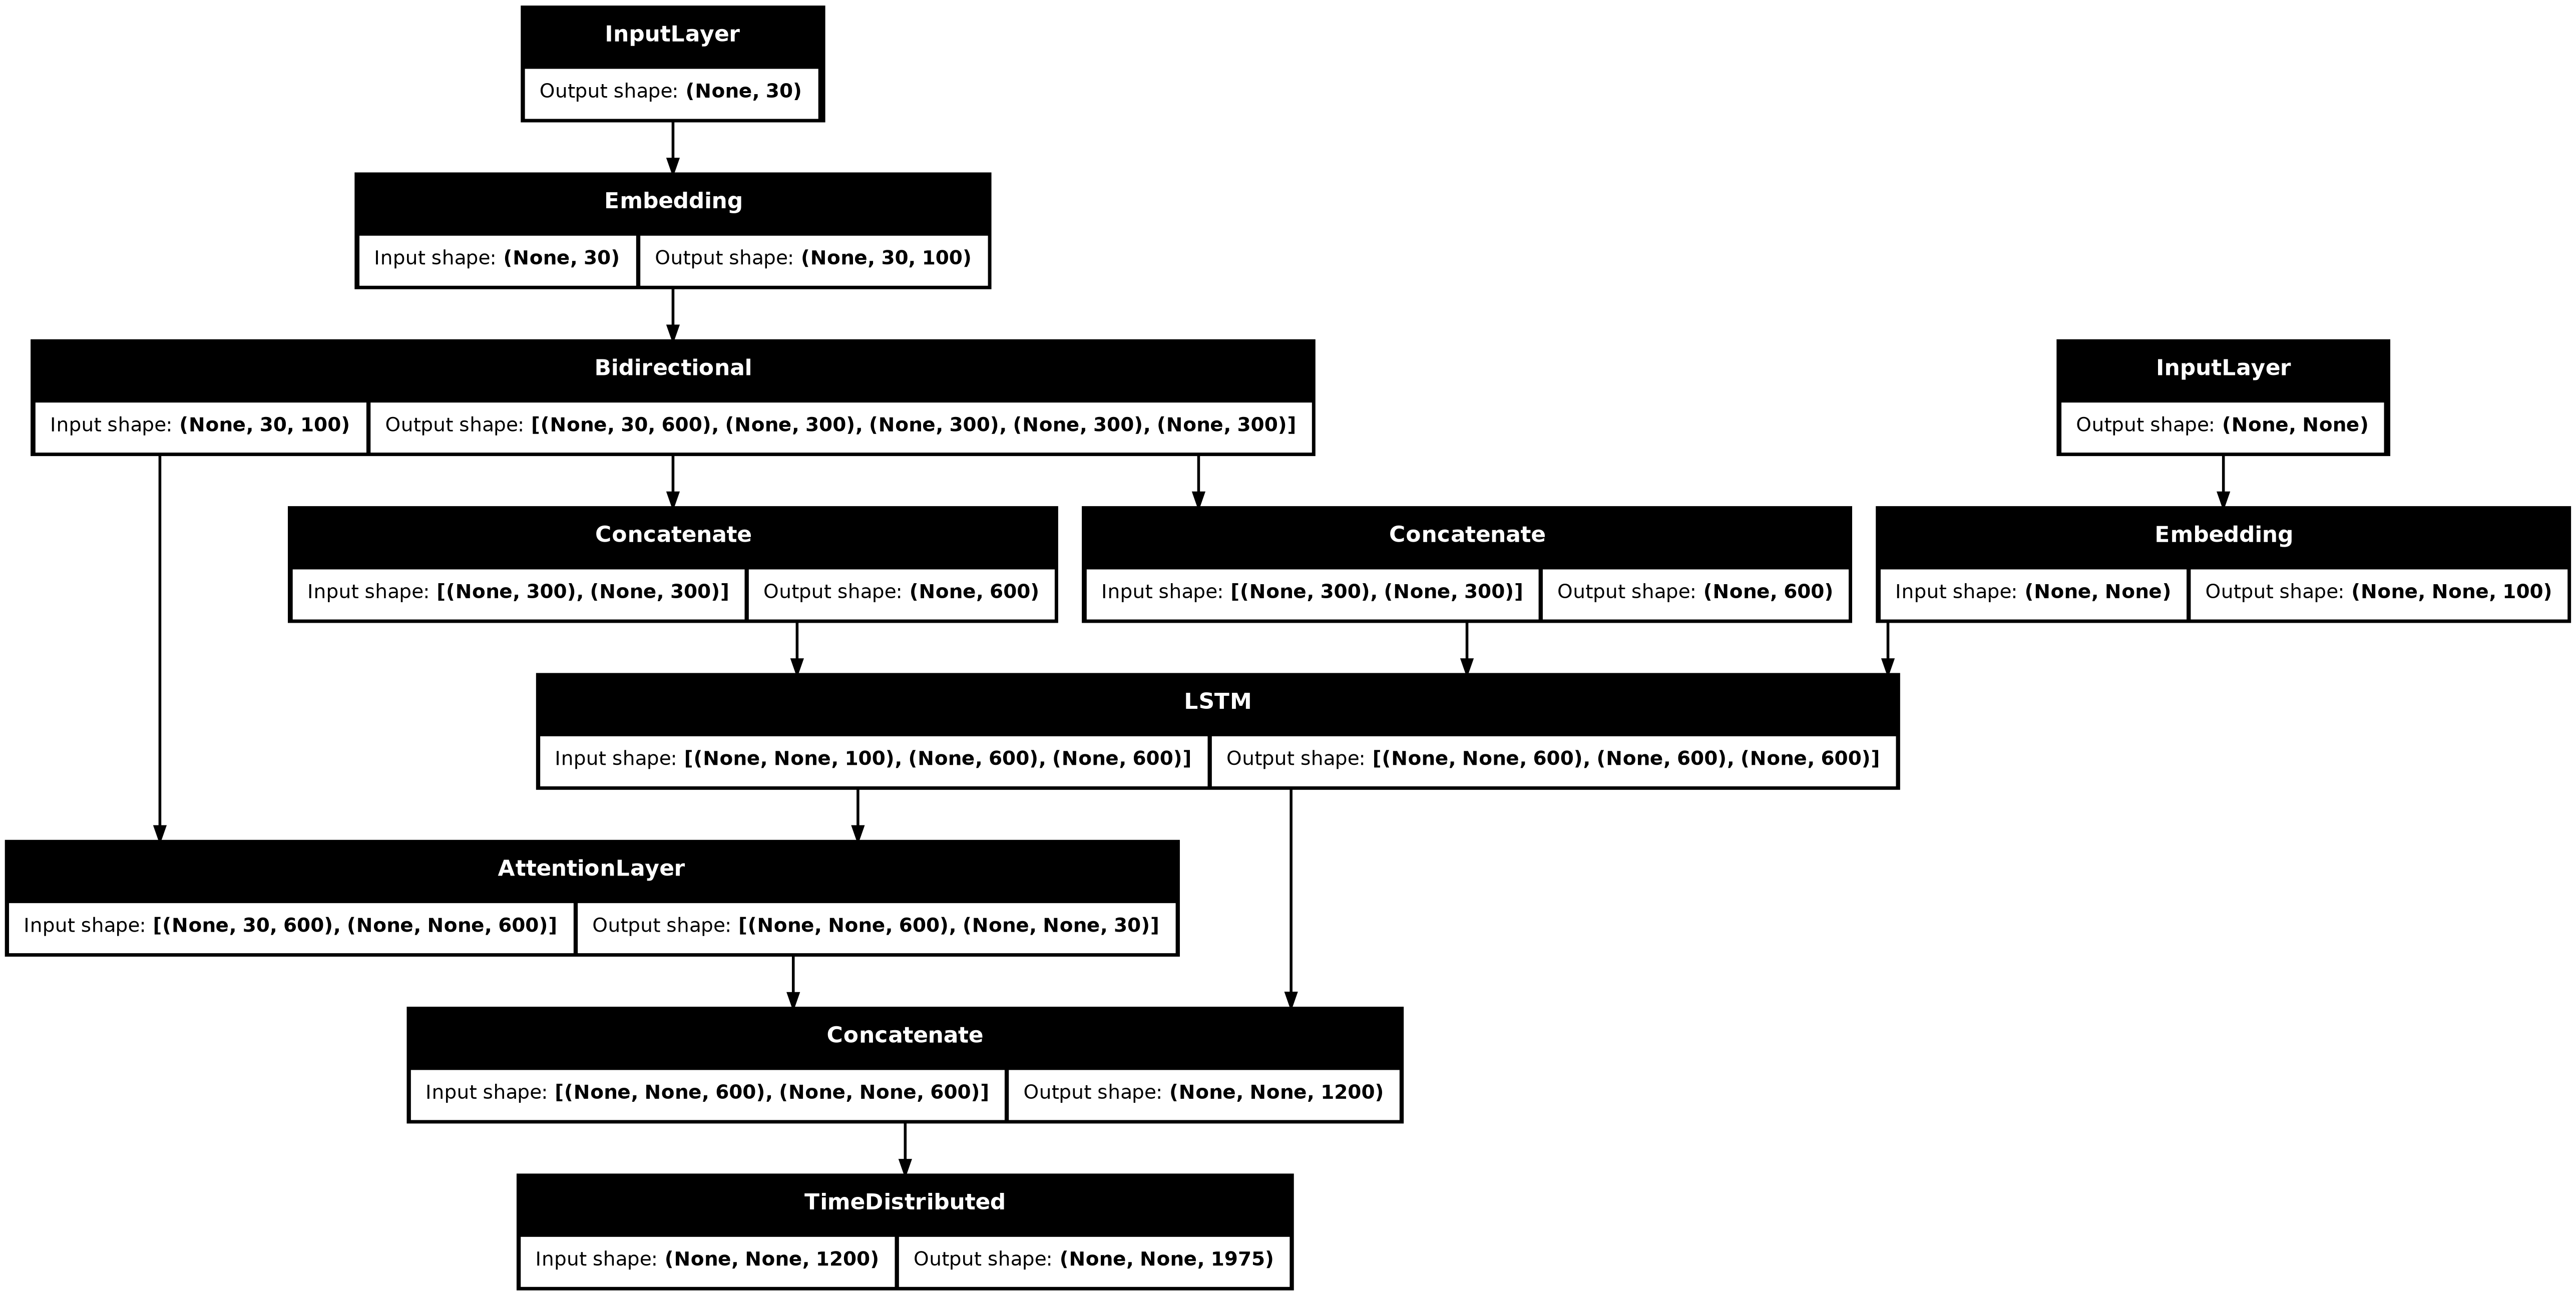
\includegraphics[width=1\textwidth]{media/Seq2SeqBiLSTM_image.png}
    \caption{Diagramma dell'architettura del modello Seq2SeqBiLSTM}
    \label{fig:biLSTM_model_architecture}
\end{figure}

\section{Training del Modello Seq2SeqBiLSTM}
Il processo di addestramento per il modello Seq2SeqBiLSTM è stato simile a quello del modello Seq2Seq LSTM, ma con l'encoder bidirezionale, che permette al modello di considerare il contesto sia precedente che successivo per ogni parola.

\subsection{Loss}
Durante l'addestramento, la loss sul training set è scesa a circa [valore loss training set], mentre la loss sul validation set è arrivata a [valore loss validation set].\\
L'andamento della loss durante l'addestramento è mostrato nella figura \ref{fig:biLSTM_loss_plot}.

\begin{figure}[H]
    \centering
    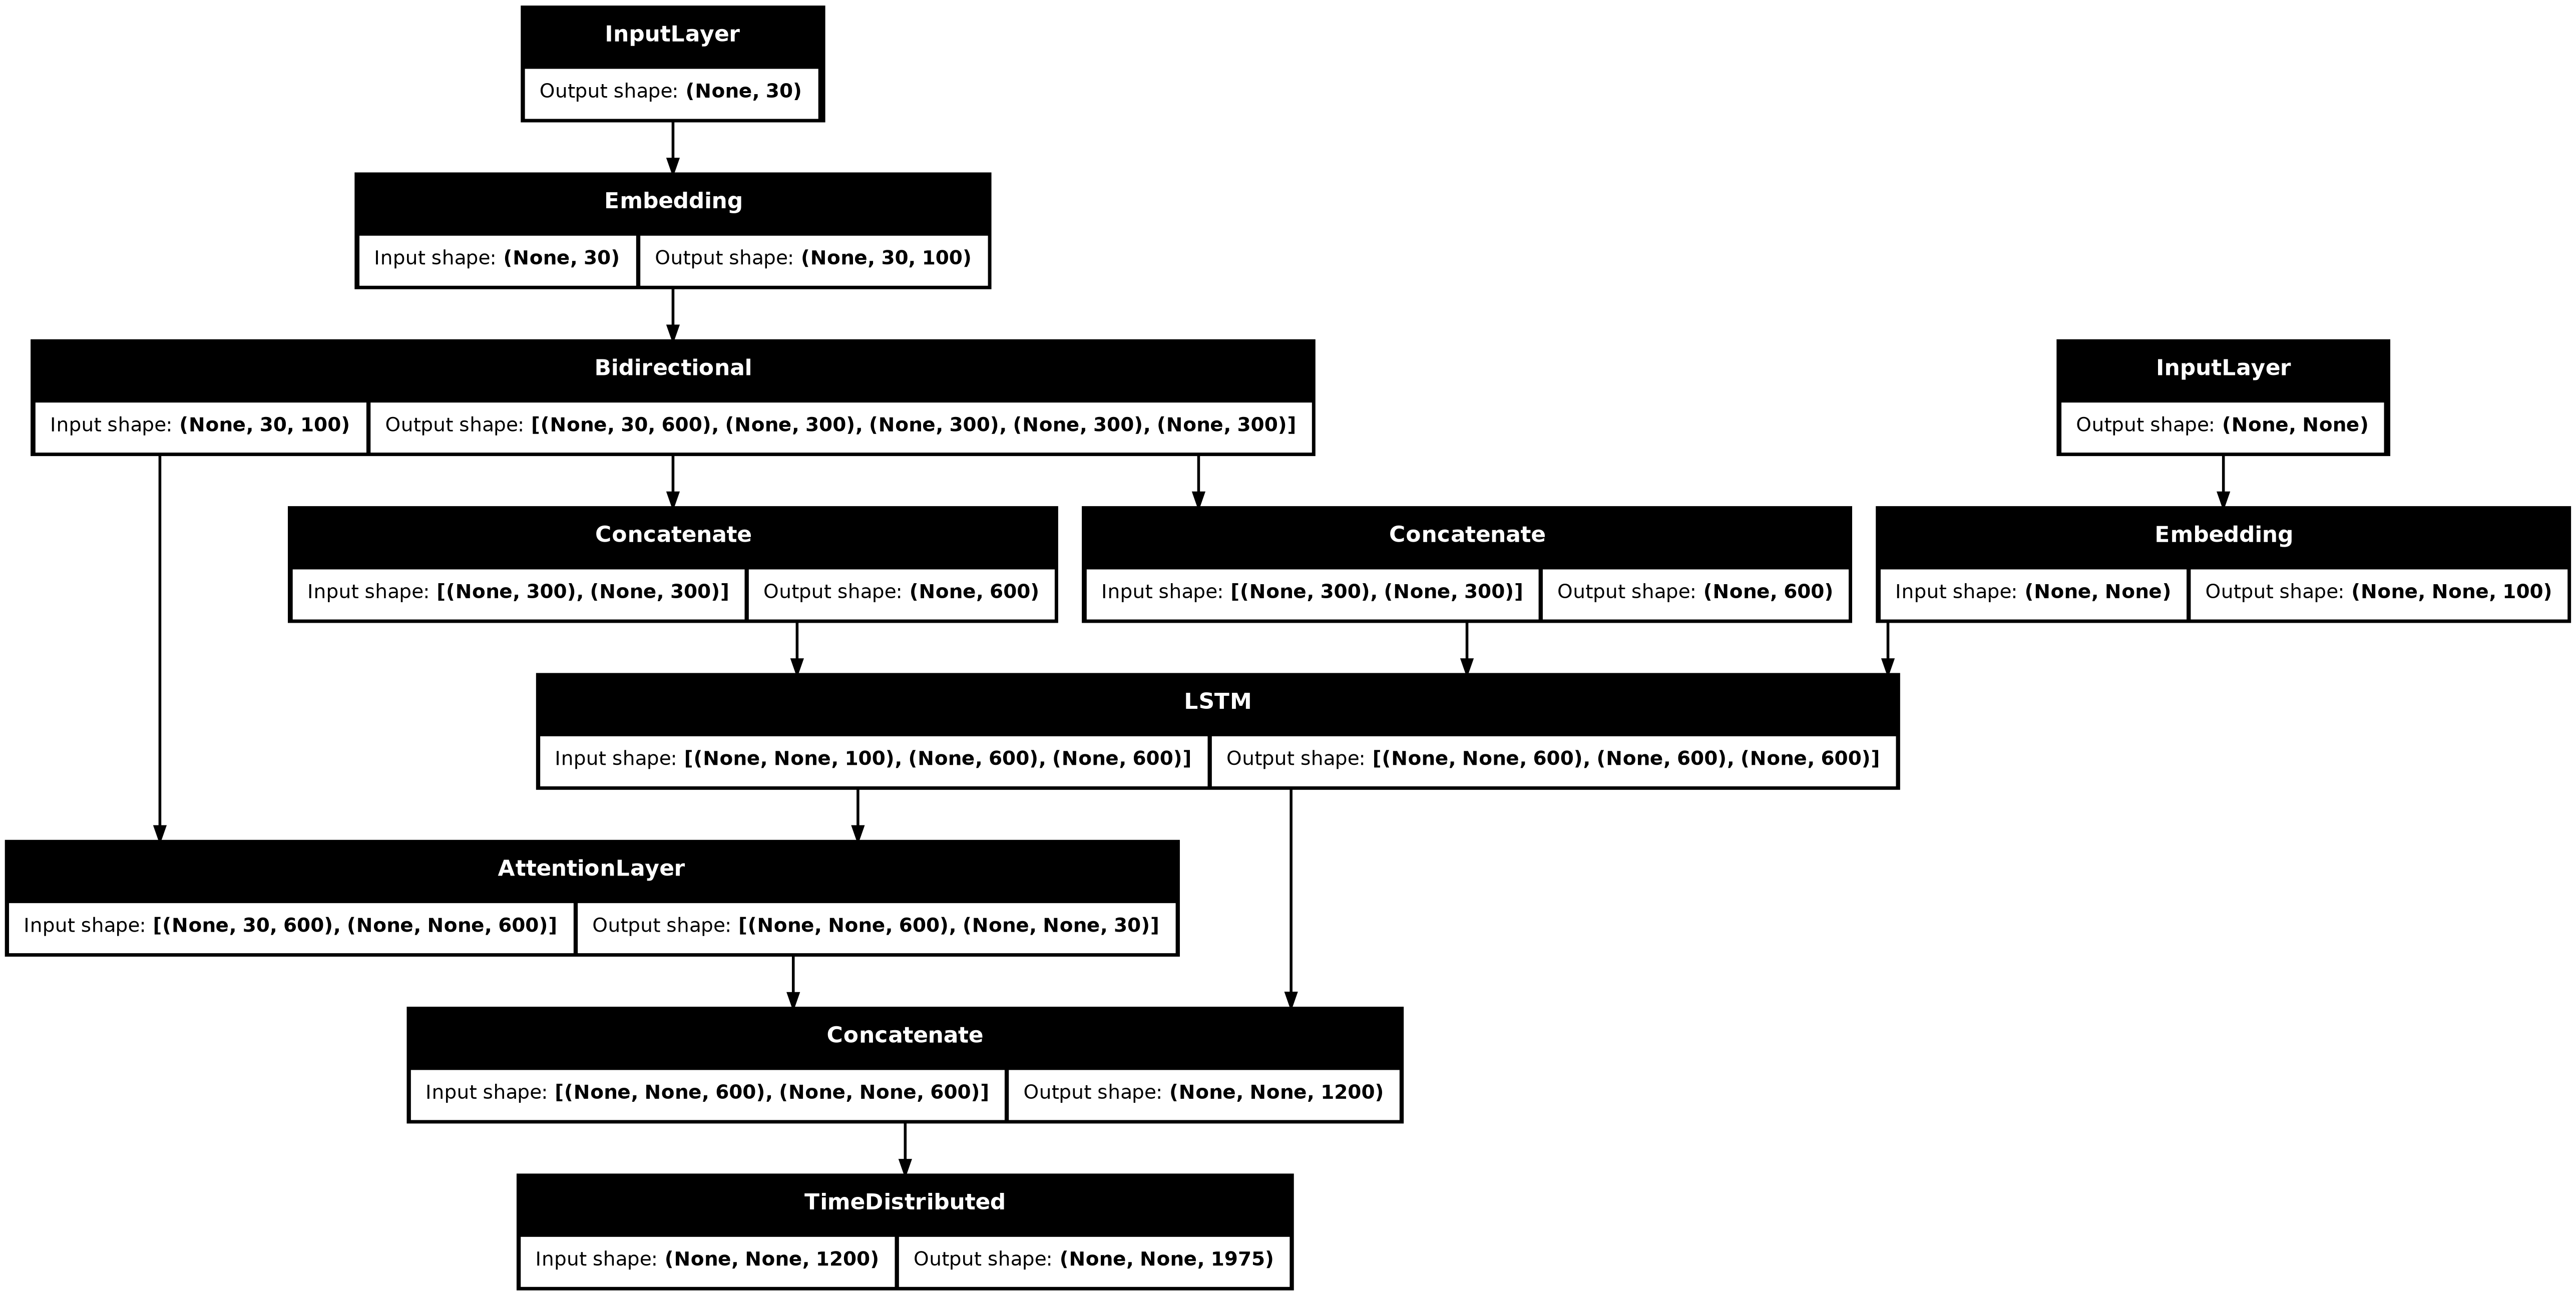
\includegraphics[width=1\textwidth]{media/Seq2SeqBiLSTM_image.png}
    \caption{Andamento delle loss durante l'addestramento per il modello Seq2SeqBiLSTM}
    \label{fig:biLSTM_loss_plot}
\end{figure}

\section{Metriche di Valutazione per Seq2SeqBiLSTM}

Come per il modello Seq2Seq LSTM, sono state calcolate le metriche ROUGE, WER, e la Similarità Cosine per valutare le performance del modello Seq2SeqBiLSTM.

\subsection{ROUGE (Recall-Oriented Understudy for Gisting Evaluation)}
I valori delle metriche ROUGE per il modello Seq2SeqBiLSTM sono mostrati nelle seguenti figure:

\begin{figure}[H]
    \centering
    \begin{subfigure}{0.32\textwidth}
        \centering
        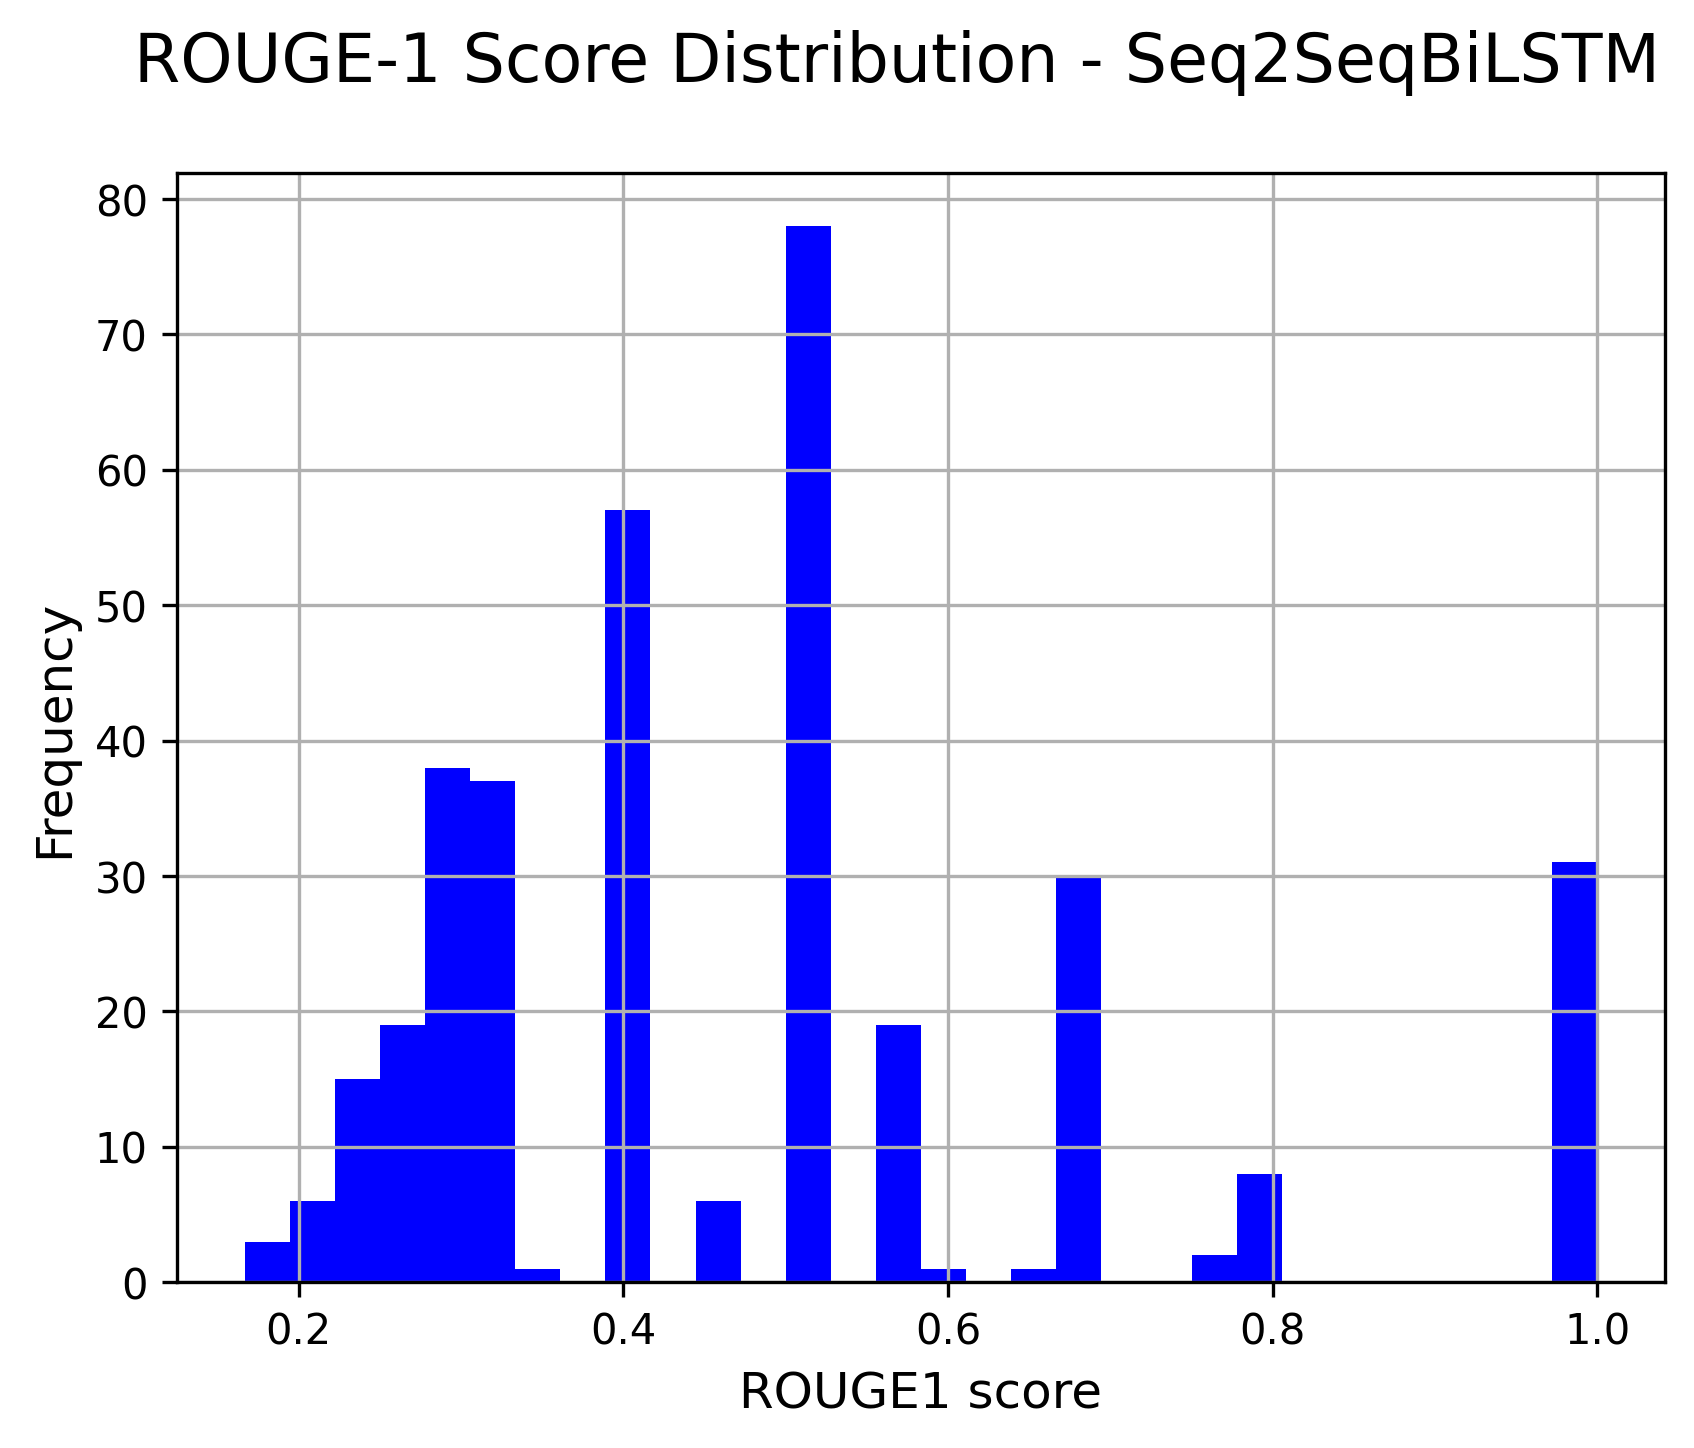
\includegraphics[width=\textwidth]{media/Seq2SeqBiLSTM_rouge1_scores.png}
        \caption{ROUGE-1}
        \label{fig:biLSTM_rouge_1}
    \end{subfigure}
    \hfill
    \begin{subfigure}{0.32\textwidth}
        \centering
        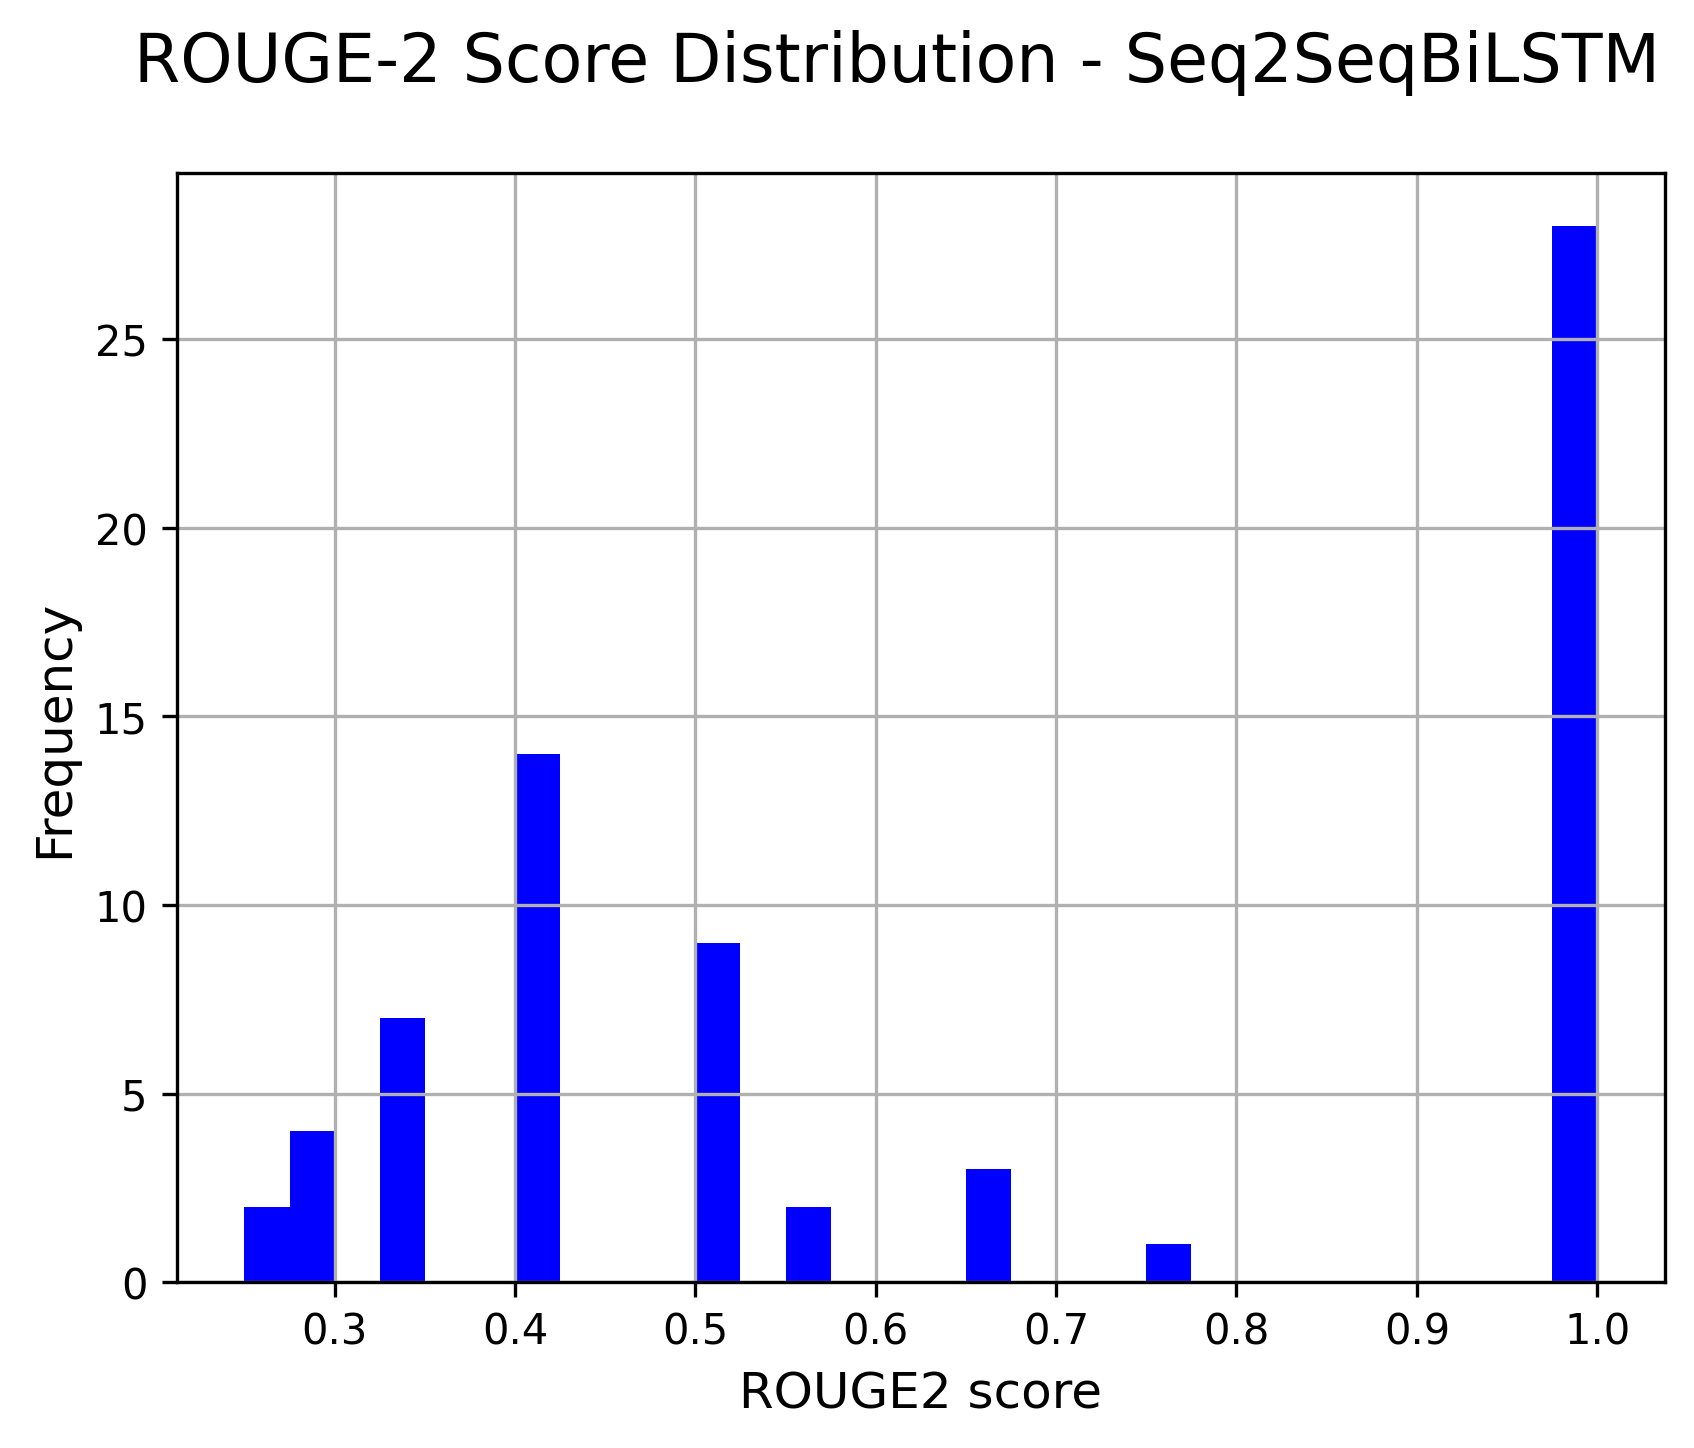
\includegraphics[width=\textwidth]{media/Seq2SeqBiLSTM_rouge2_scores.png}
        \caption{ROUGE-2}
        \label{fig:biLSTM_rouge_2}
    \end{subfigure}
    \hfill
    \begin{subfigure}{0.32\textwidth}
        \centering
        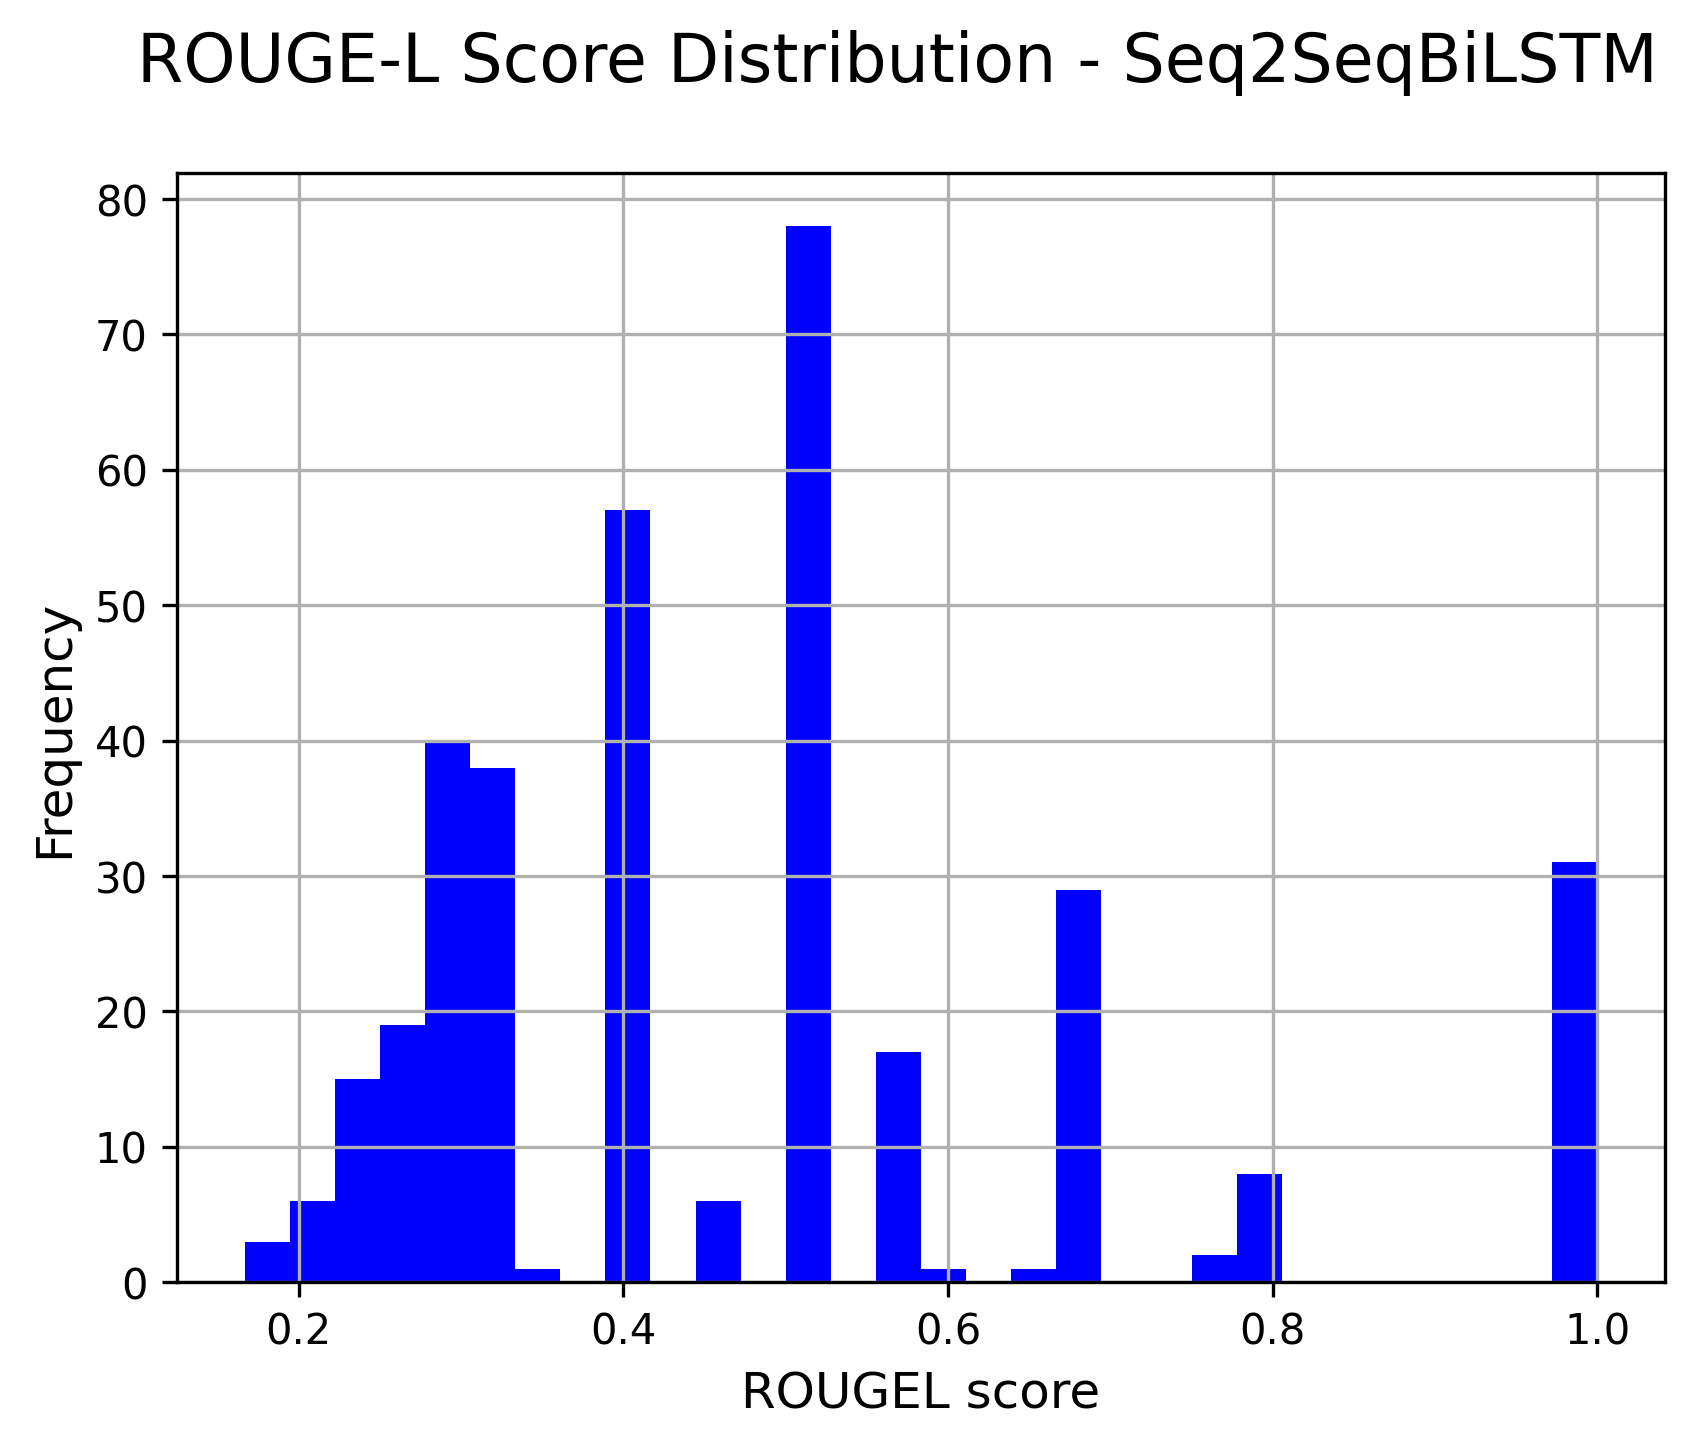
\includegraphics[width=\textwidth]{media/Seq2SeqBiLSTM_rougeL_scores.png}
        \caption{ROUGE-L}
        \label{fig:biLSTM_rouge_l}
    \end{subfigure}
    \caption{Valori ROUGE per il modello Seq2SeqBiLSTM: (a) ROUGE-1, (b) ROUGE-2, and (c) ROUGE-L.}
    \label{fig:biLSTM_rouge_scores}
\end{figure}

\subsection{Word Error Rate (WER)}
Il WER per il modello Seq2SeqBiLSTM è stato calcolato sui riassunti generati e i riassunti di riferimento.\\
I valori di WER sono mostrati nella figura \ref{fig:biLSTM_wer}.

\begin{figure}[H]
    \centering
    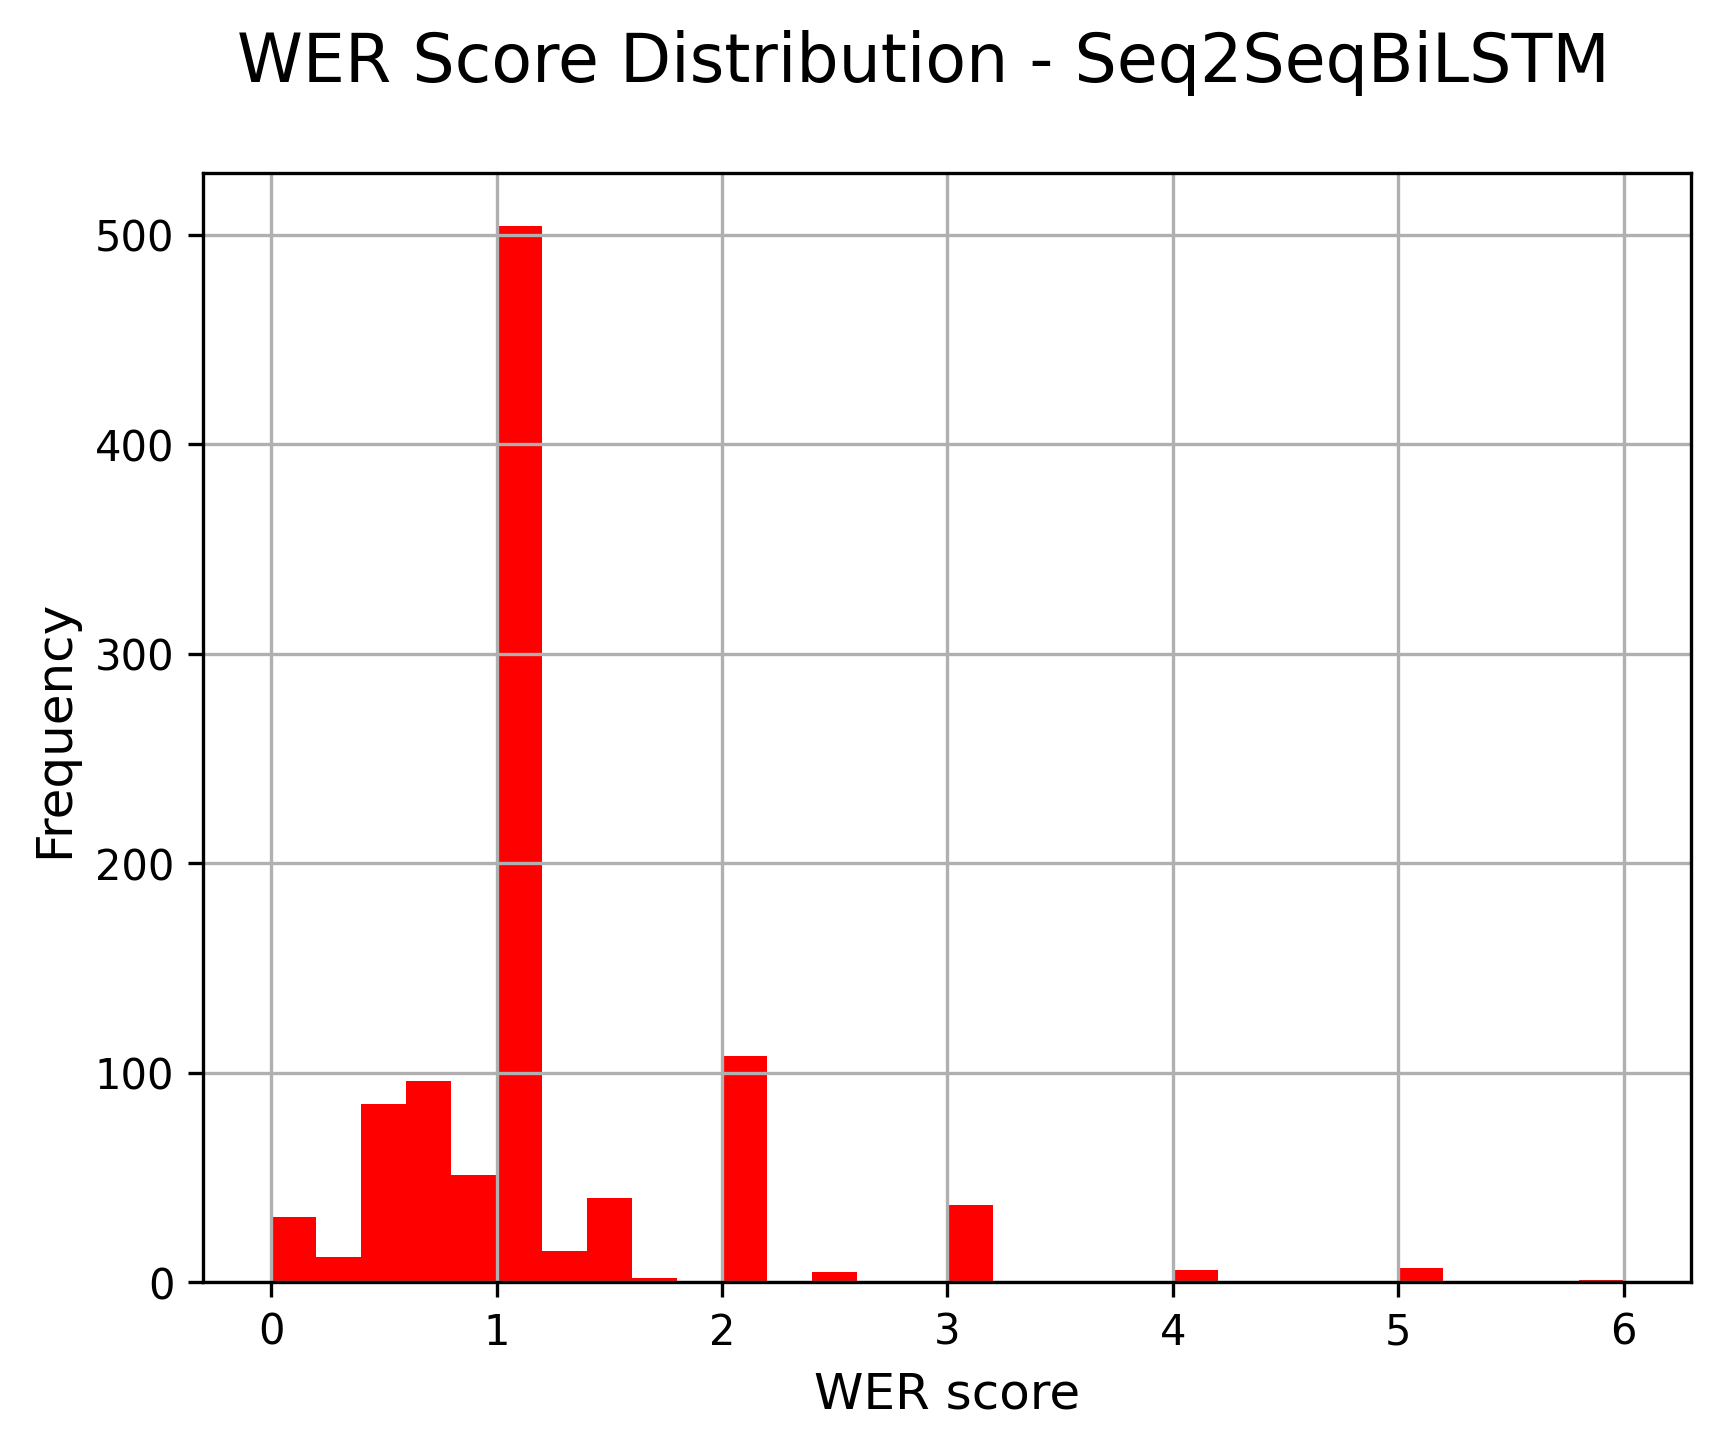
\includegraphics[width=0.75\textwidth]{media/Seq2SeqBiLSTM_wer_scores.png}
    \caption{Valori WER per il modello Seq2SeqBiLSTM}
    \label{fig:biLSTM_wer}
\end{figure}

\subsection{Cosine Similarity}
La similarità cosenica per il modello Seq2SeqBiLSTM è stata calcolata tra i vettori di embedding delle parole nei riassunti generati e quelli nei riassunti di riferimento.\\
I valori di similarità cosenica sono mostrati nella figura \ref{fig:biLSTM_cosine_similarity}.

\begin{figure}[H]
    \centering
    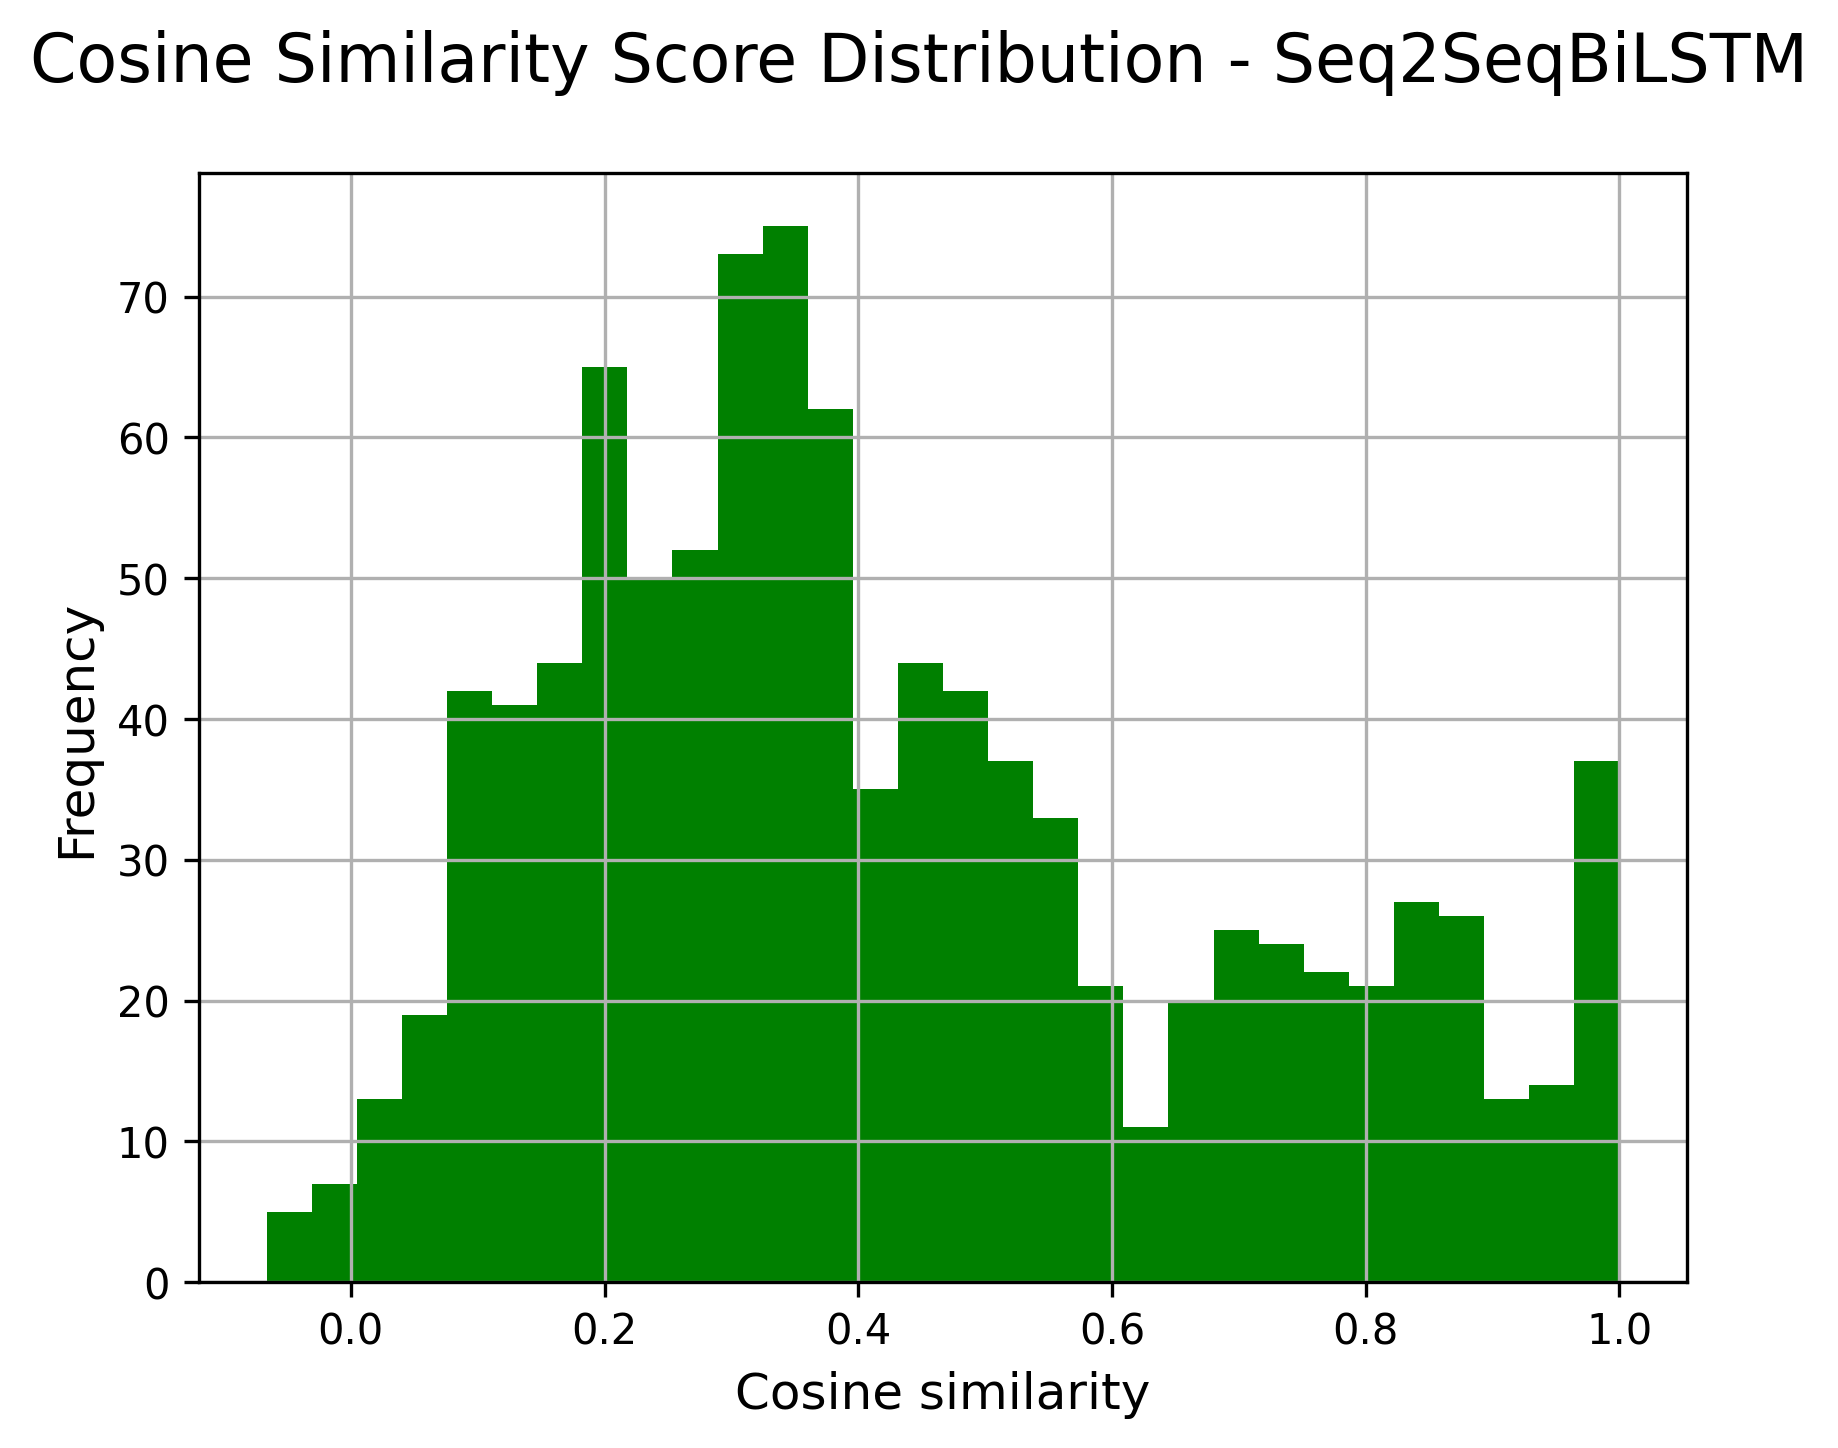
\includegraphics[width=0.75\textwidth]{media/Seq2SeqBiLSTM_cosine_similarity_scores.png}
    \caption{Valori di similarità cosenica per il modello Seq2SeqBiLSTM}
    \label{fig:biLSTM_cosine_similarity}
\end{figure}

\section{Confronto tra Seq2SeqLSTM e Seq2SeqBiLSTM}
In questa sezione vengono confrontate le prestazioni dei due modelli utilizzando i grafici delle metriche di valutazione: ROUGE, WER e cosine similarity.

\subsection{ROUGE Scores}
I grafici nella Figura \ref{fig:rouge_comparison} confrontano le performance in termini di ROUGE-1, ROUGE-2 e ROUGE-L per i due modelli. Il modello Seq2SeqBiLSTM mostra un miglioramento nei punteggi ROUGE rispetto al Seq2SeqLSTM, indicando una maggiore capacità di catturare similarità lessicali.

\begin{figure}[H]
    \centering
    \begin{subfigure}{0.32\textwidth}
        \centering
        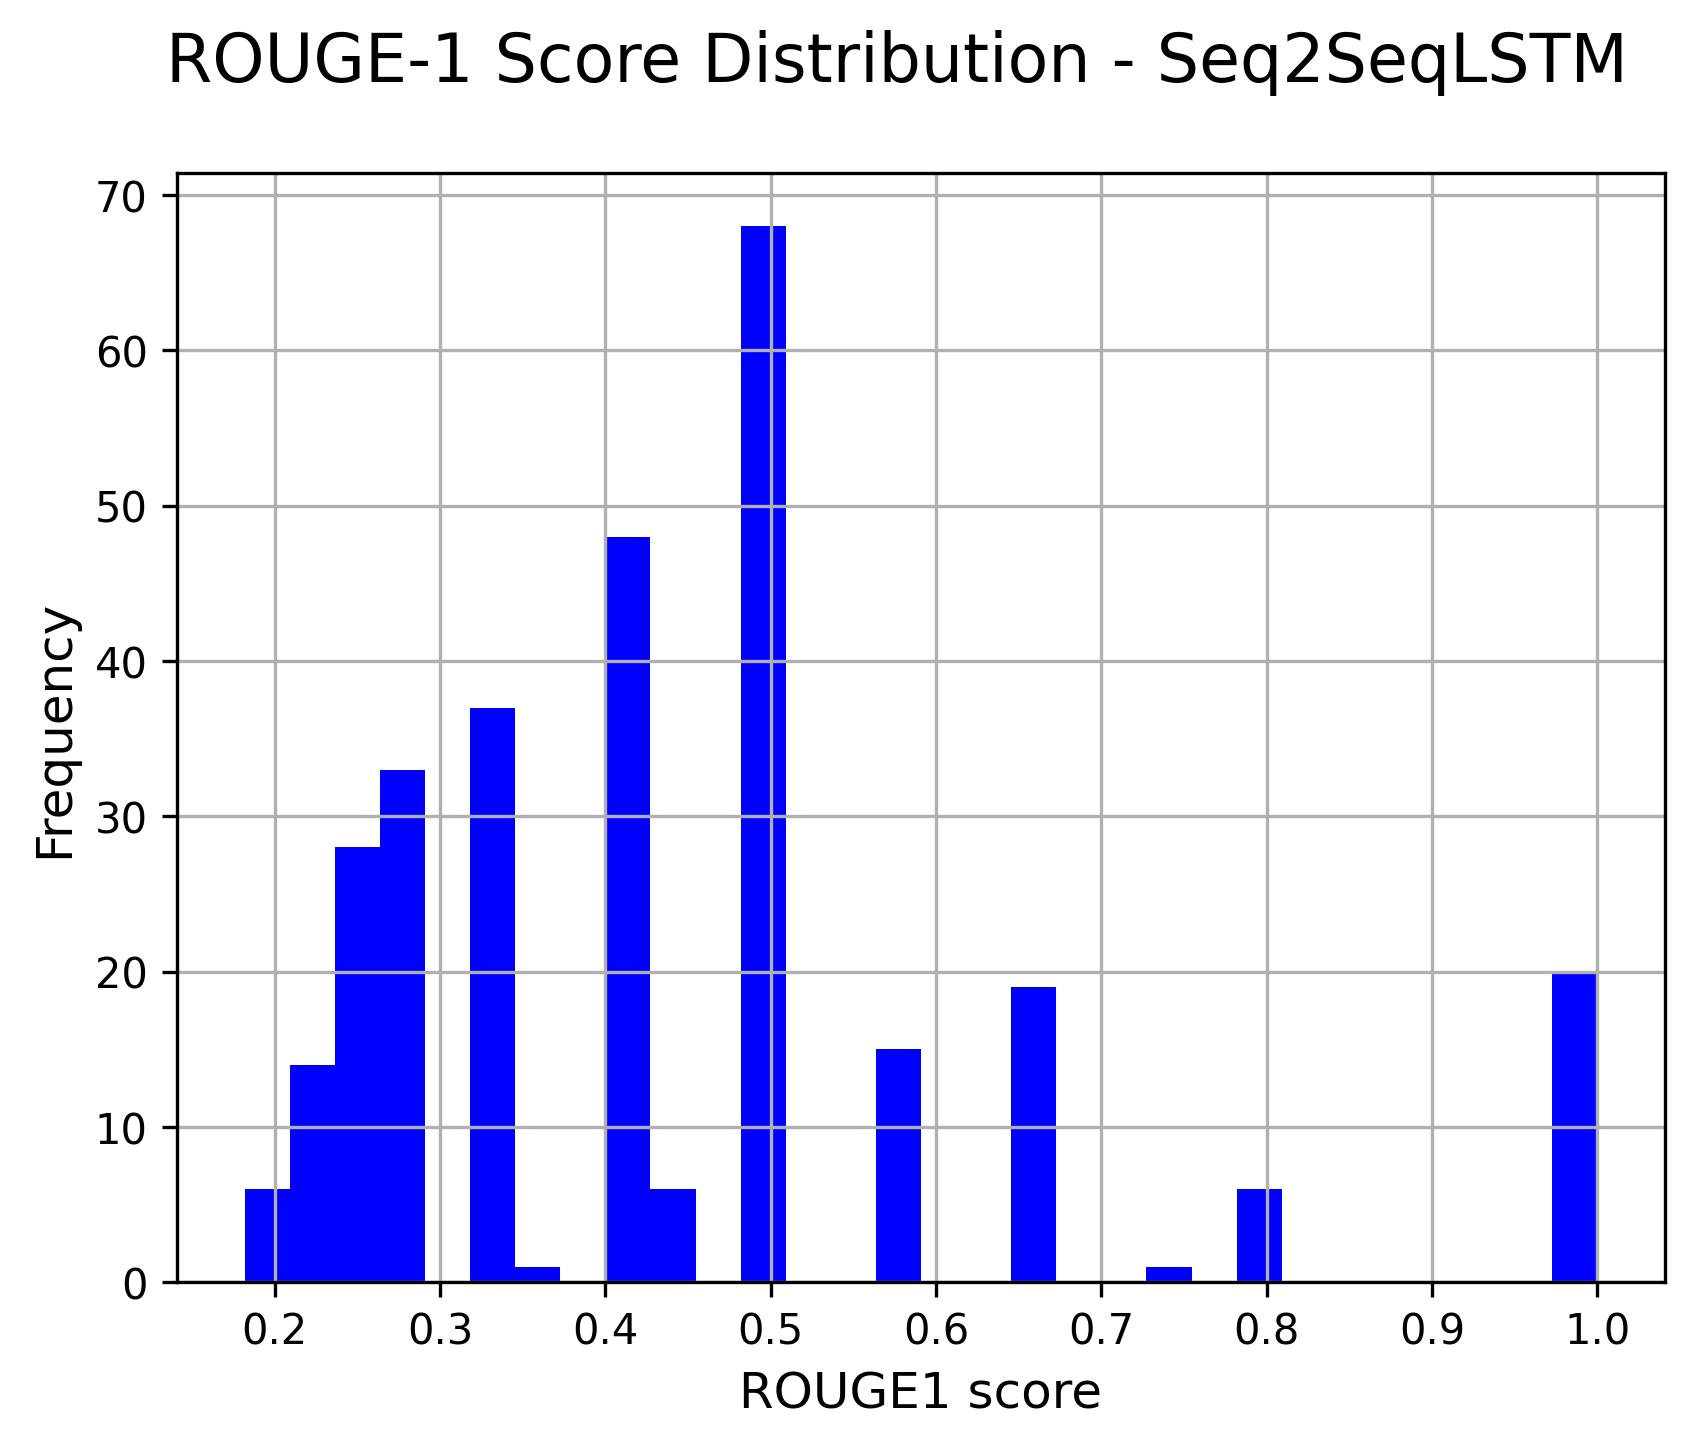
\includegraphics[width=\textwidth]{media/Seq2SeqLSTM_rouge1_scores.png}
        \caption{ROUGE-1 Seq2SeqLSTM}
    \end{subfigure}
    \hfill
    \begin{subfigure}{0.32\textwidth}
        \centering
        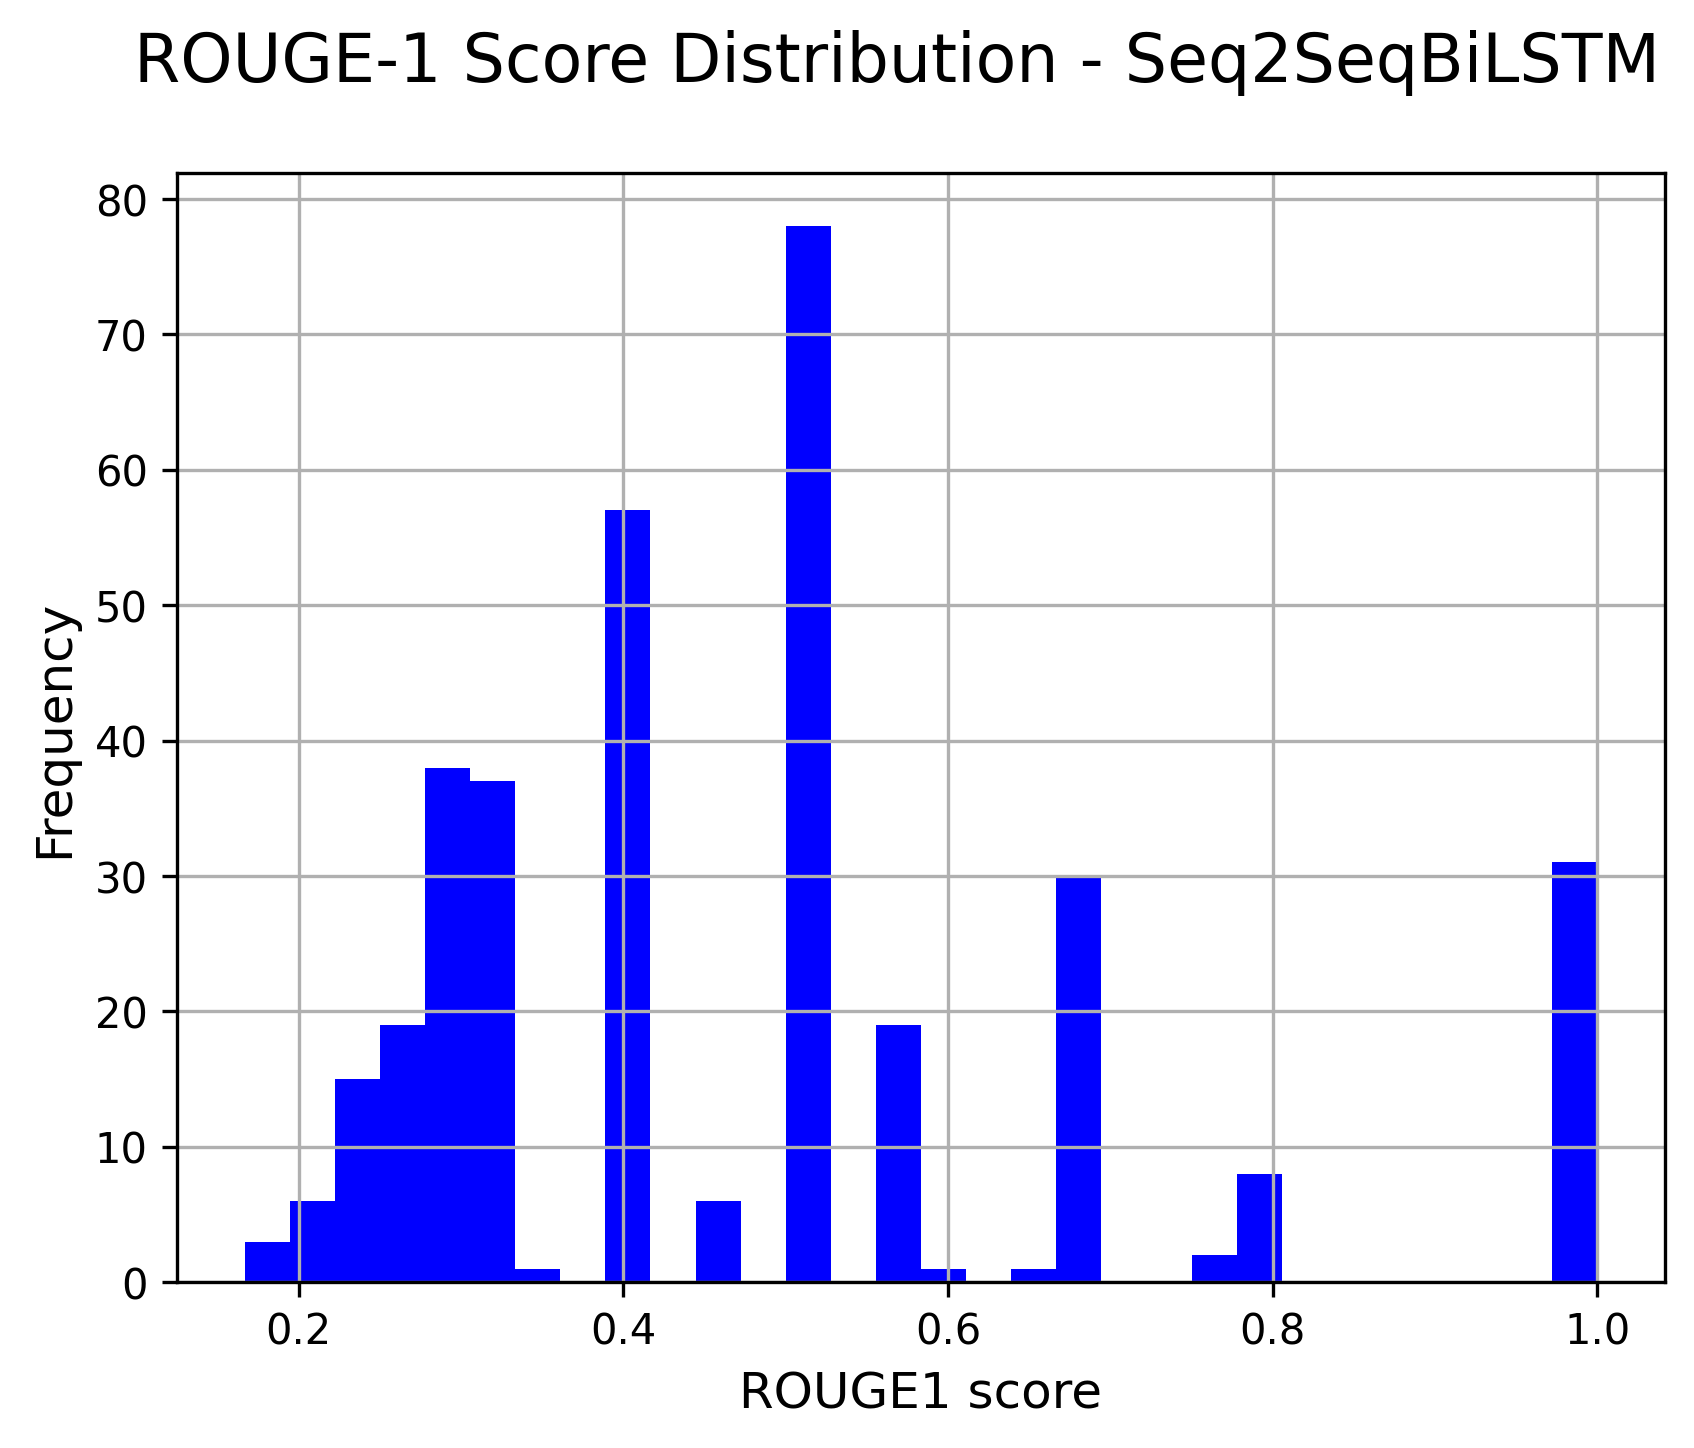
\includegraphics[width=\textwidth]{media/Seq2SeqBiLSTM_rouge1_scores.png}
        \caption{ROUGE-1 Seq2SeqBiLSTM}
    \end{subfigure}
    
    \begin{subfigure}{0.32\textwidth}
        \centering
        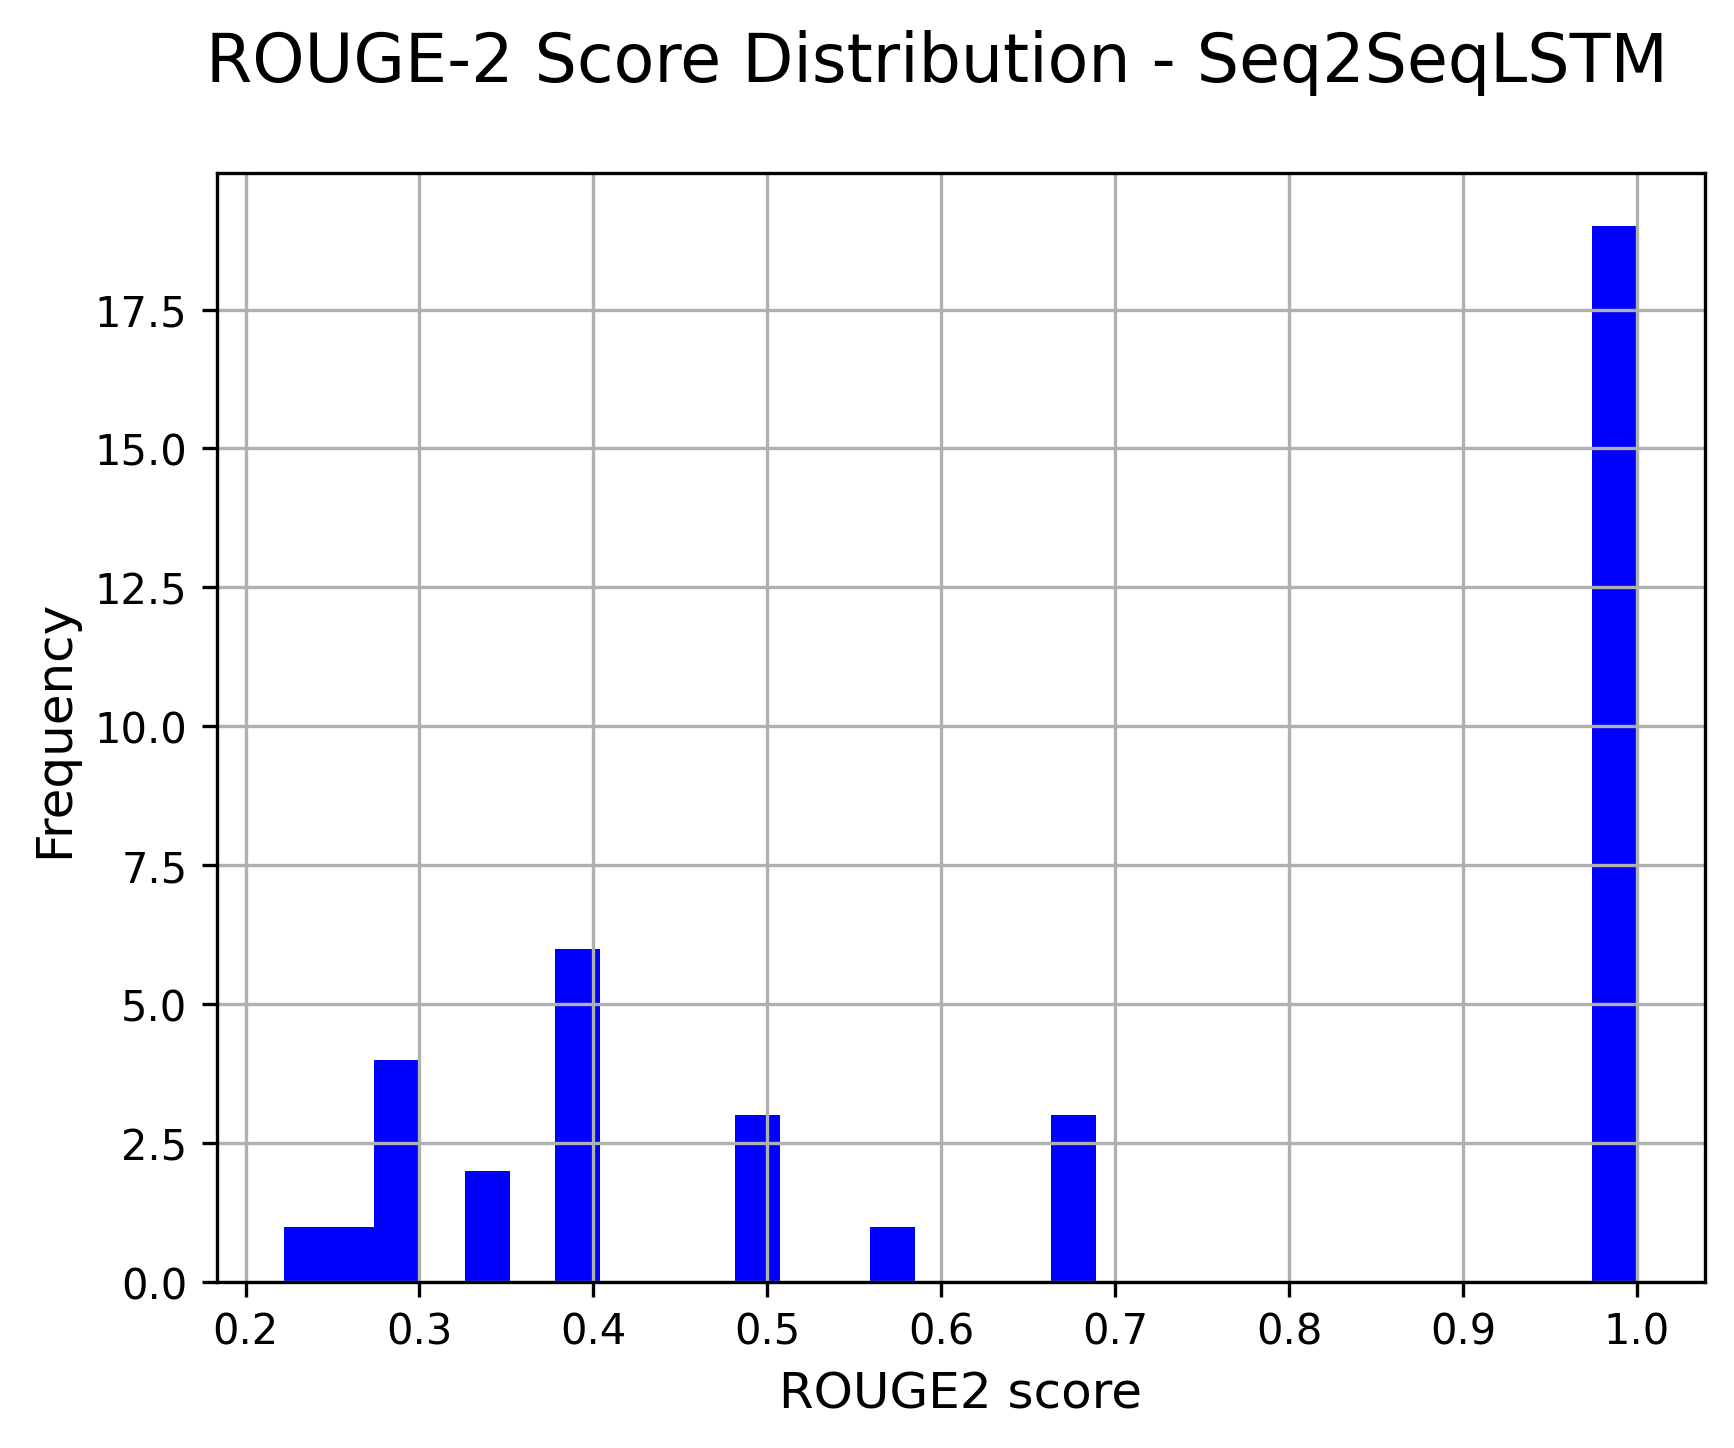
\includegraphics[width=\textwidth]{media/Seq2SeqLSTM_rouge2_scores.png}
        \caption{ROUGE-2 Seq2SeqLSTM}
    \end{subfigure}
    \hfill
    \begin{subfigure}{0.32\textwidth}
        \centering
        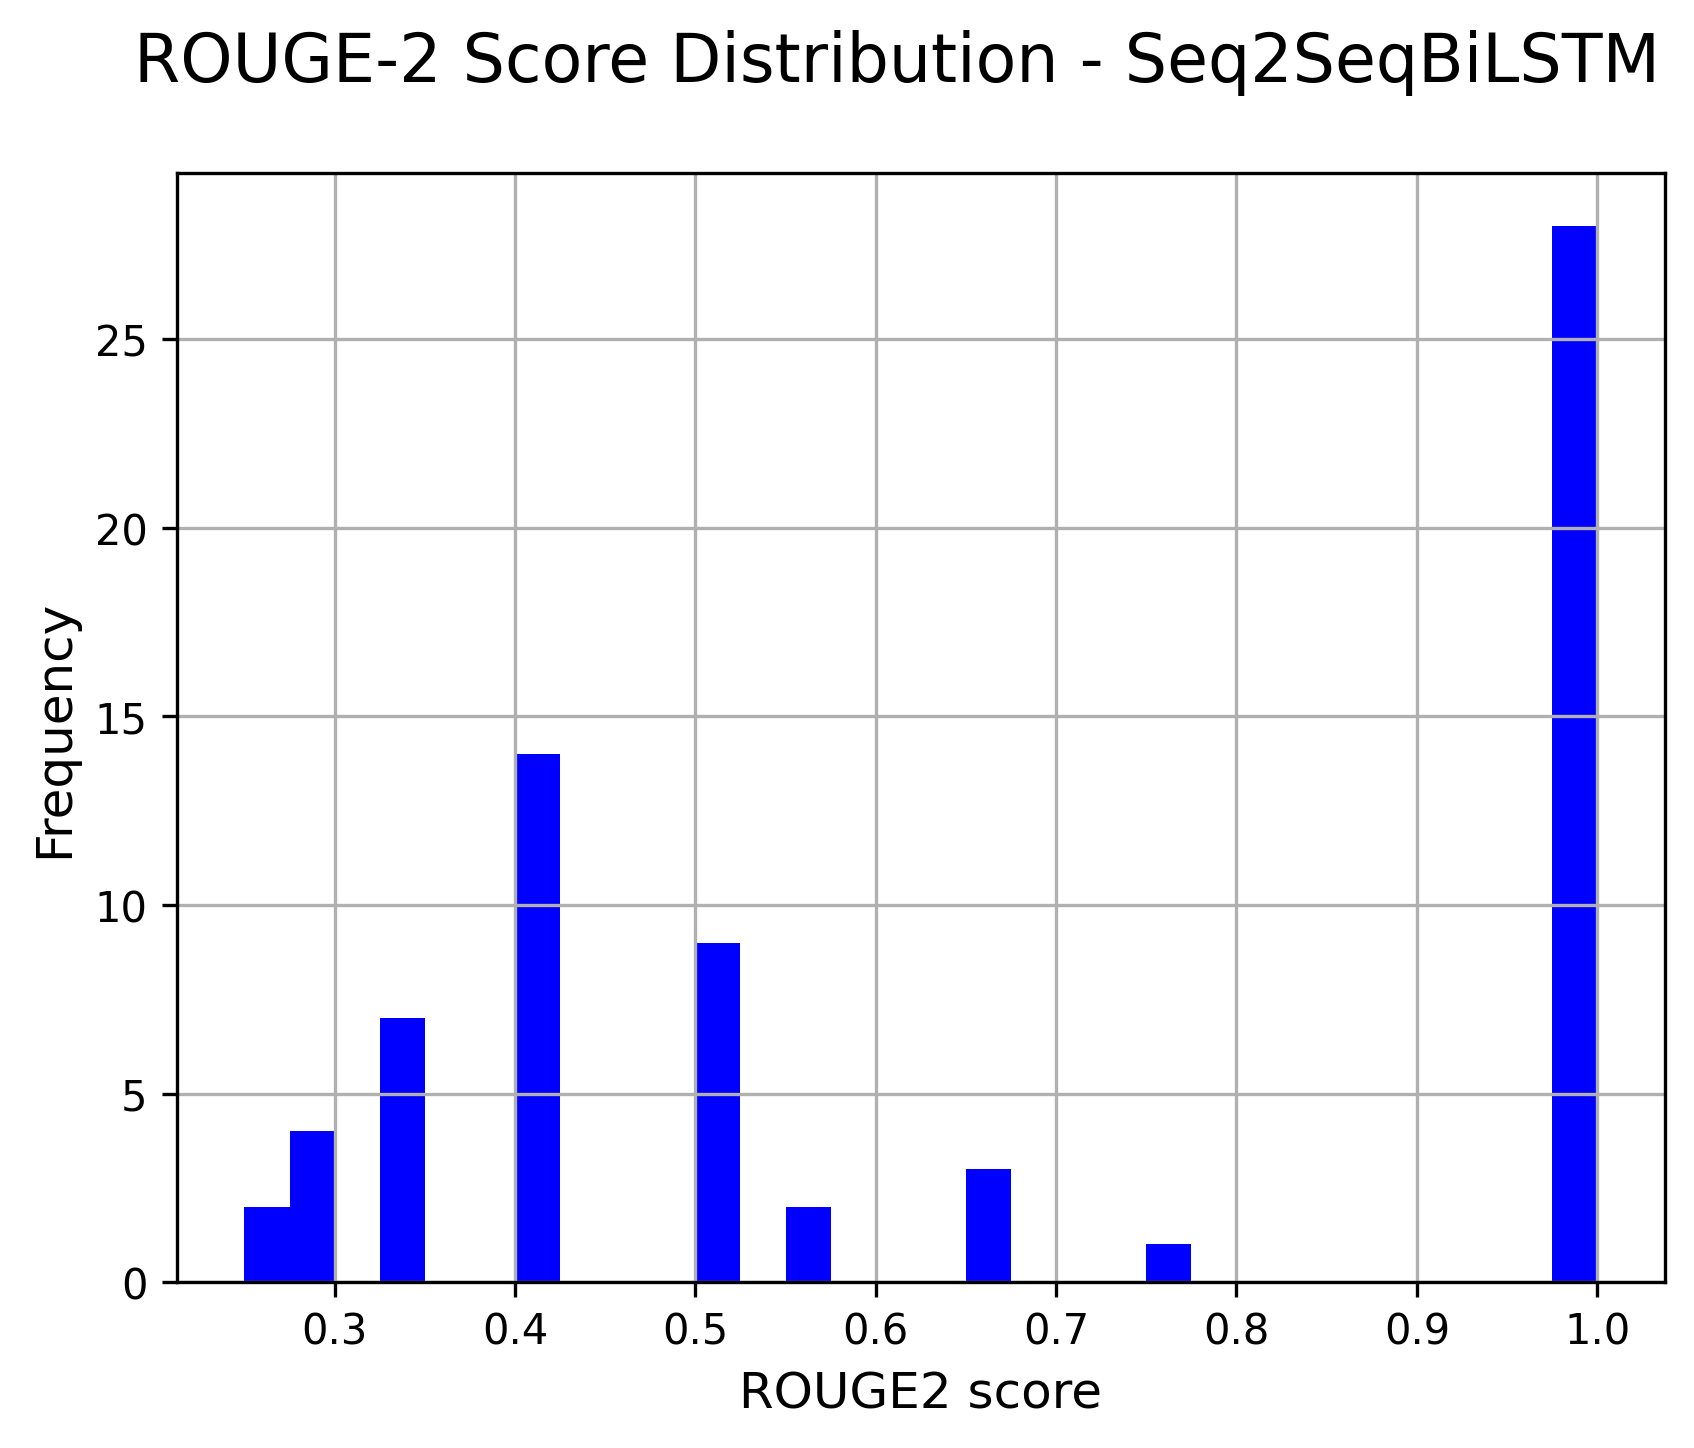
\includegraphics[width=\textwidth]{media/Seq2SeqBiLSTM_rouge2_scores.png}
        \caption{ROUGE-2 Seq2SeqBiLSTM}
    \end{subfigure}
    
    \begin{subfigure}{0.32\textwidth}
        \centering
        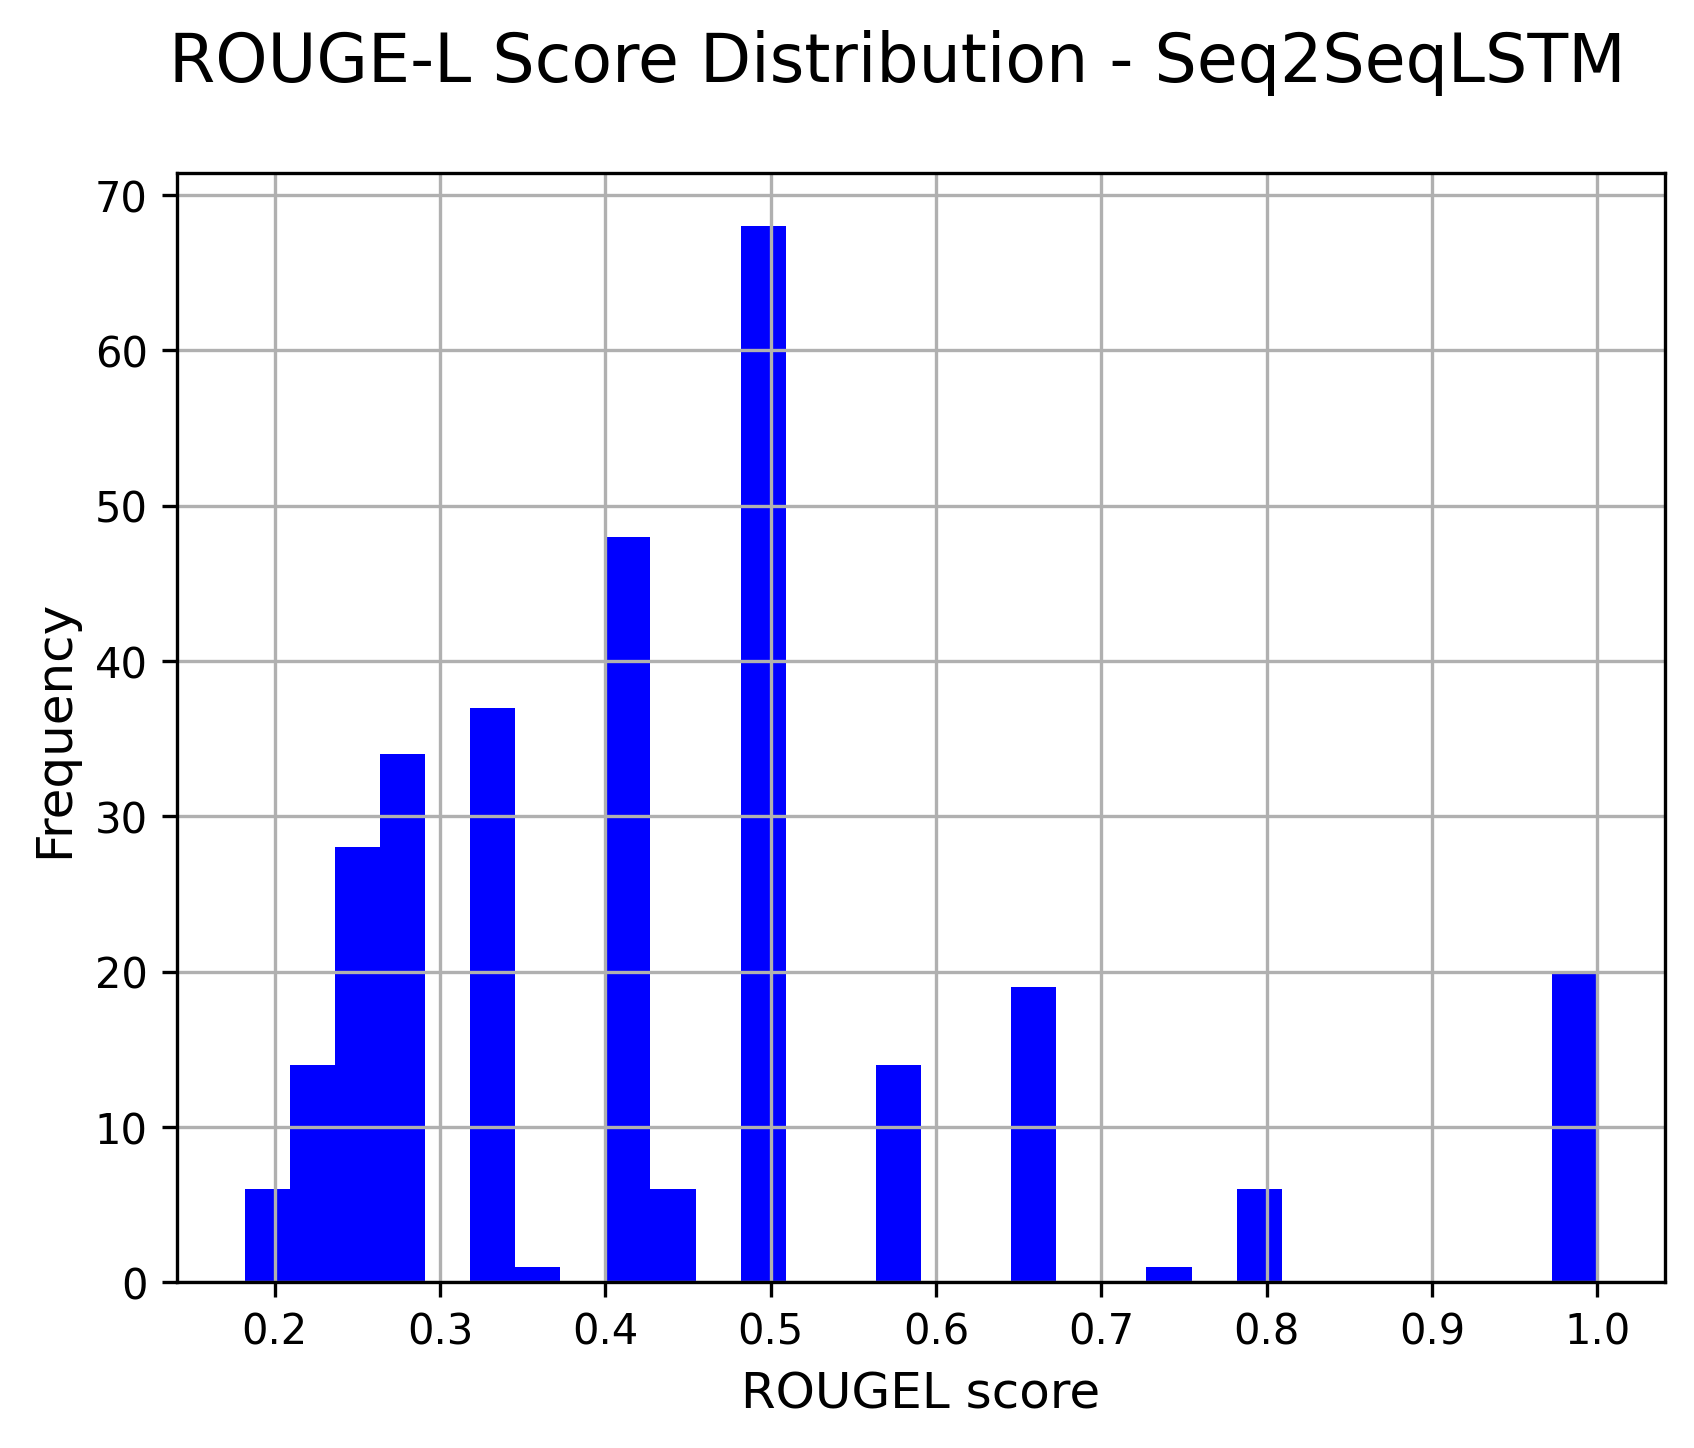
\includegraphics[width=\textwidth]{media/Seq2SeqLSTM_rougeL_scores.png}
        \caption{ROUGE-L Seq2SeqLSTM}
    \end{subfigure}
    \hfill
    \begin{subfigure}{0.32\textwidth}
        \centering
        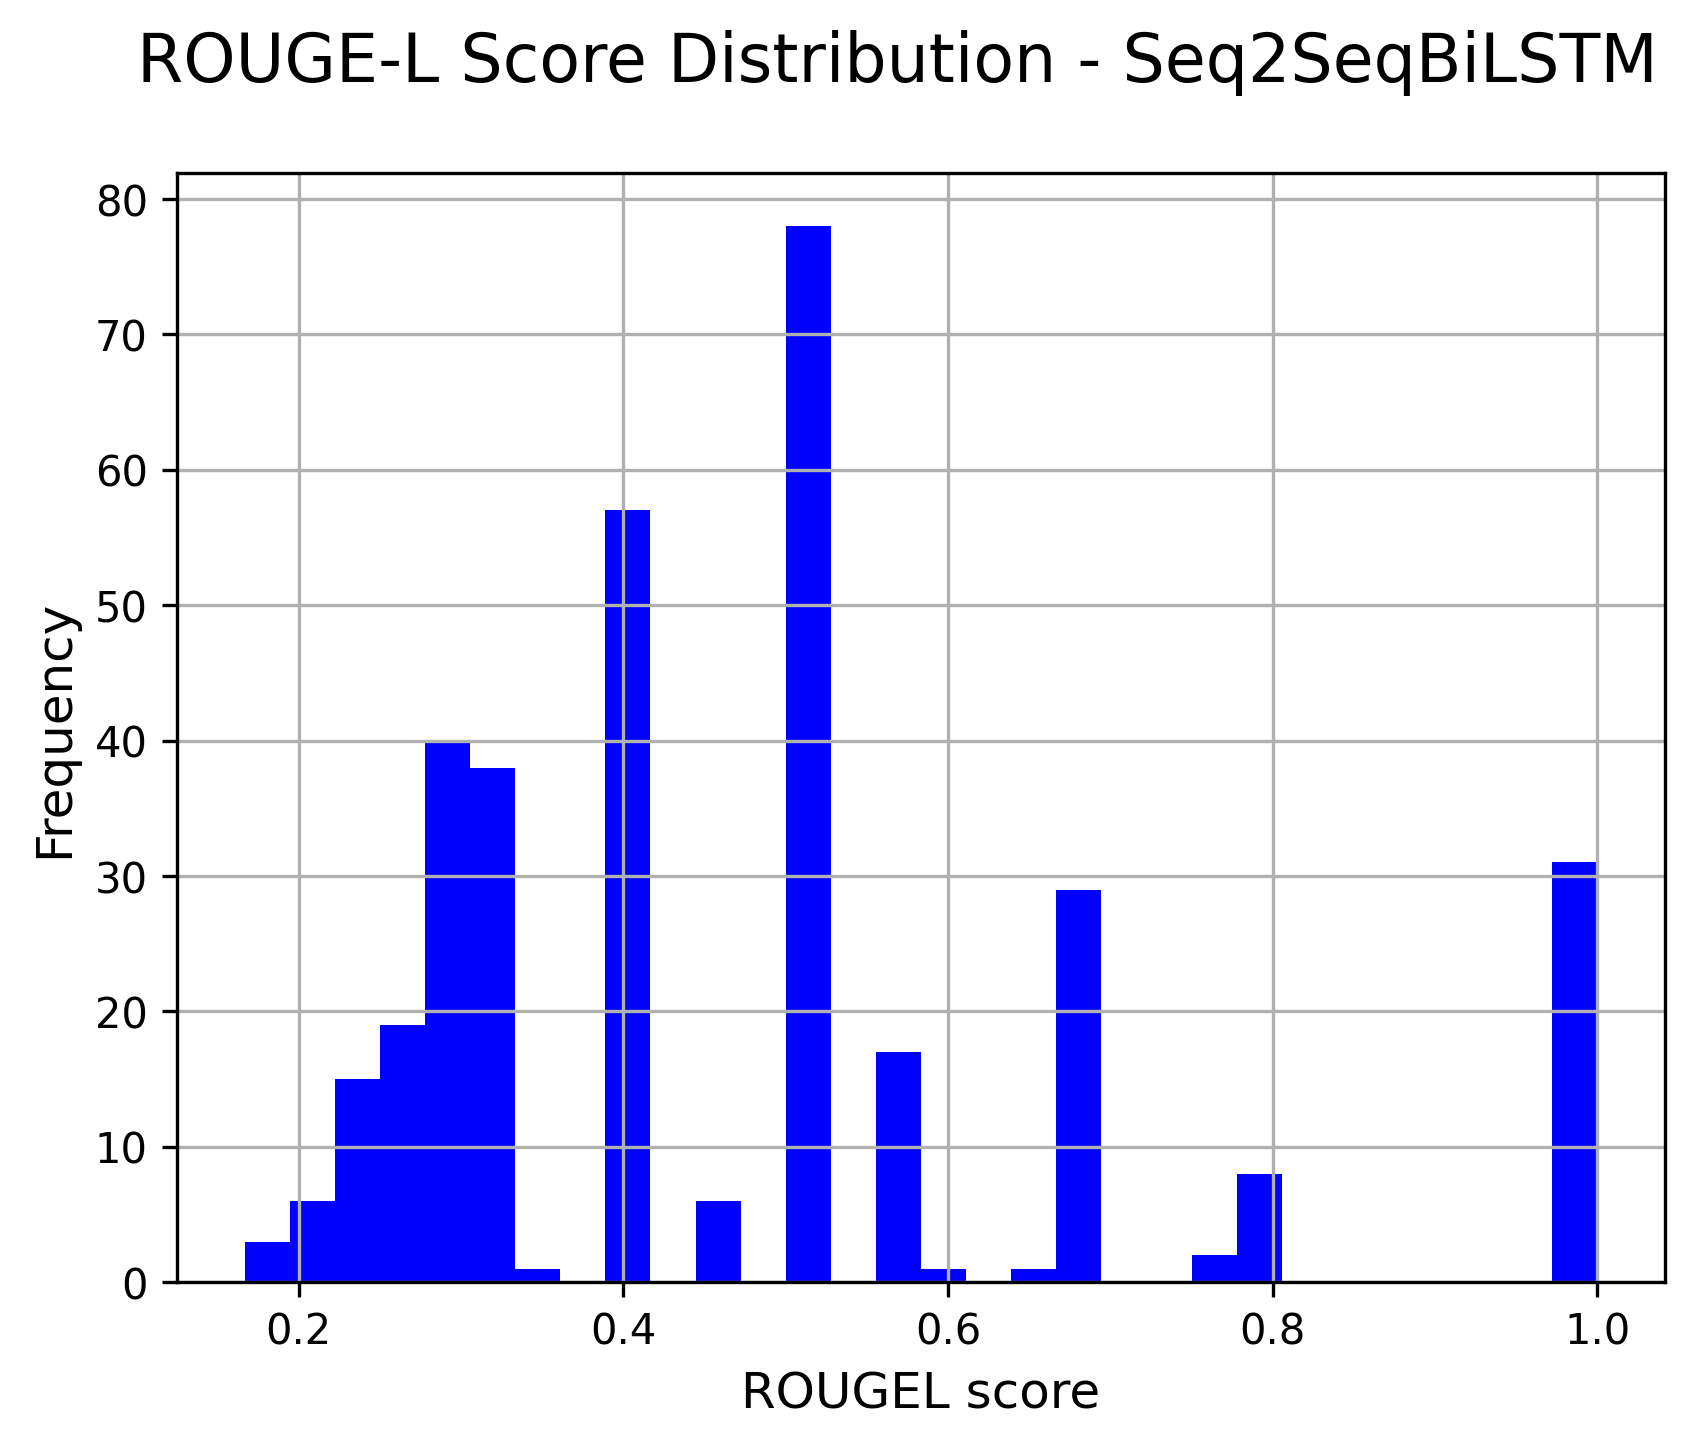
\includegraphics[width=\textwidth]{media/Seq2SeqBiLSTM_rougeL_scores.png}
        \caption{ROUGE-L Seq2SeqBiLSTM}
    \end{subfigure}
    \caption{Confronto dei punteggi ROUGE tra i modelli Seq2SeqLSTM e Seq2SeqBiLSTM.}
    \label{fig:rouge_comparison}
\end{figure}

\subsection{Word Error Rate (WER)}
Il confronto del WER, mostrato nella Figura \ref{fig:wer_comparison}, evidenzia che il modello Seq2SeqBiLSTM ottiene risultati migliori, indicando una maggiore accuratezza nella generazione delle parole.

\begin{figure}[H]
    \centering
    \begin{subfigure}{0.45\textwidth}
        \centering
        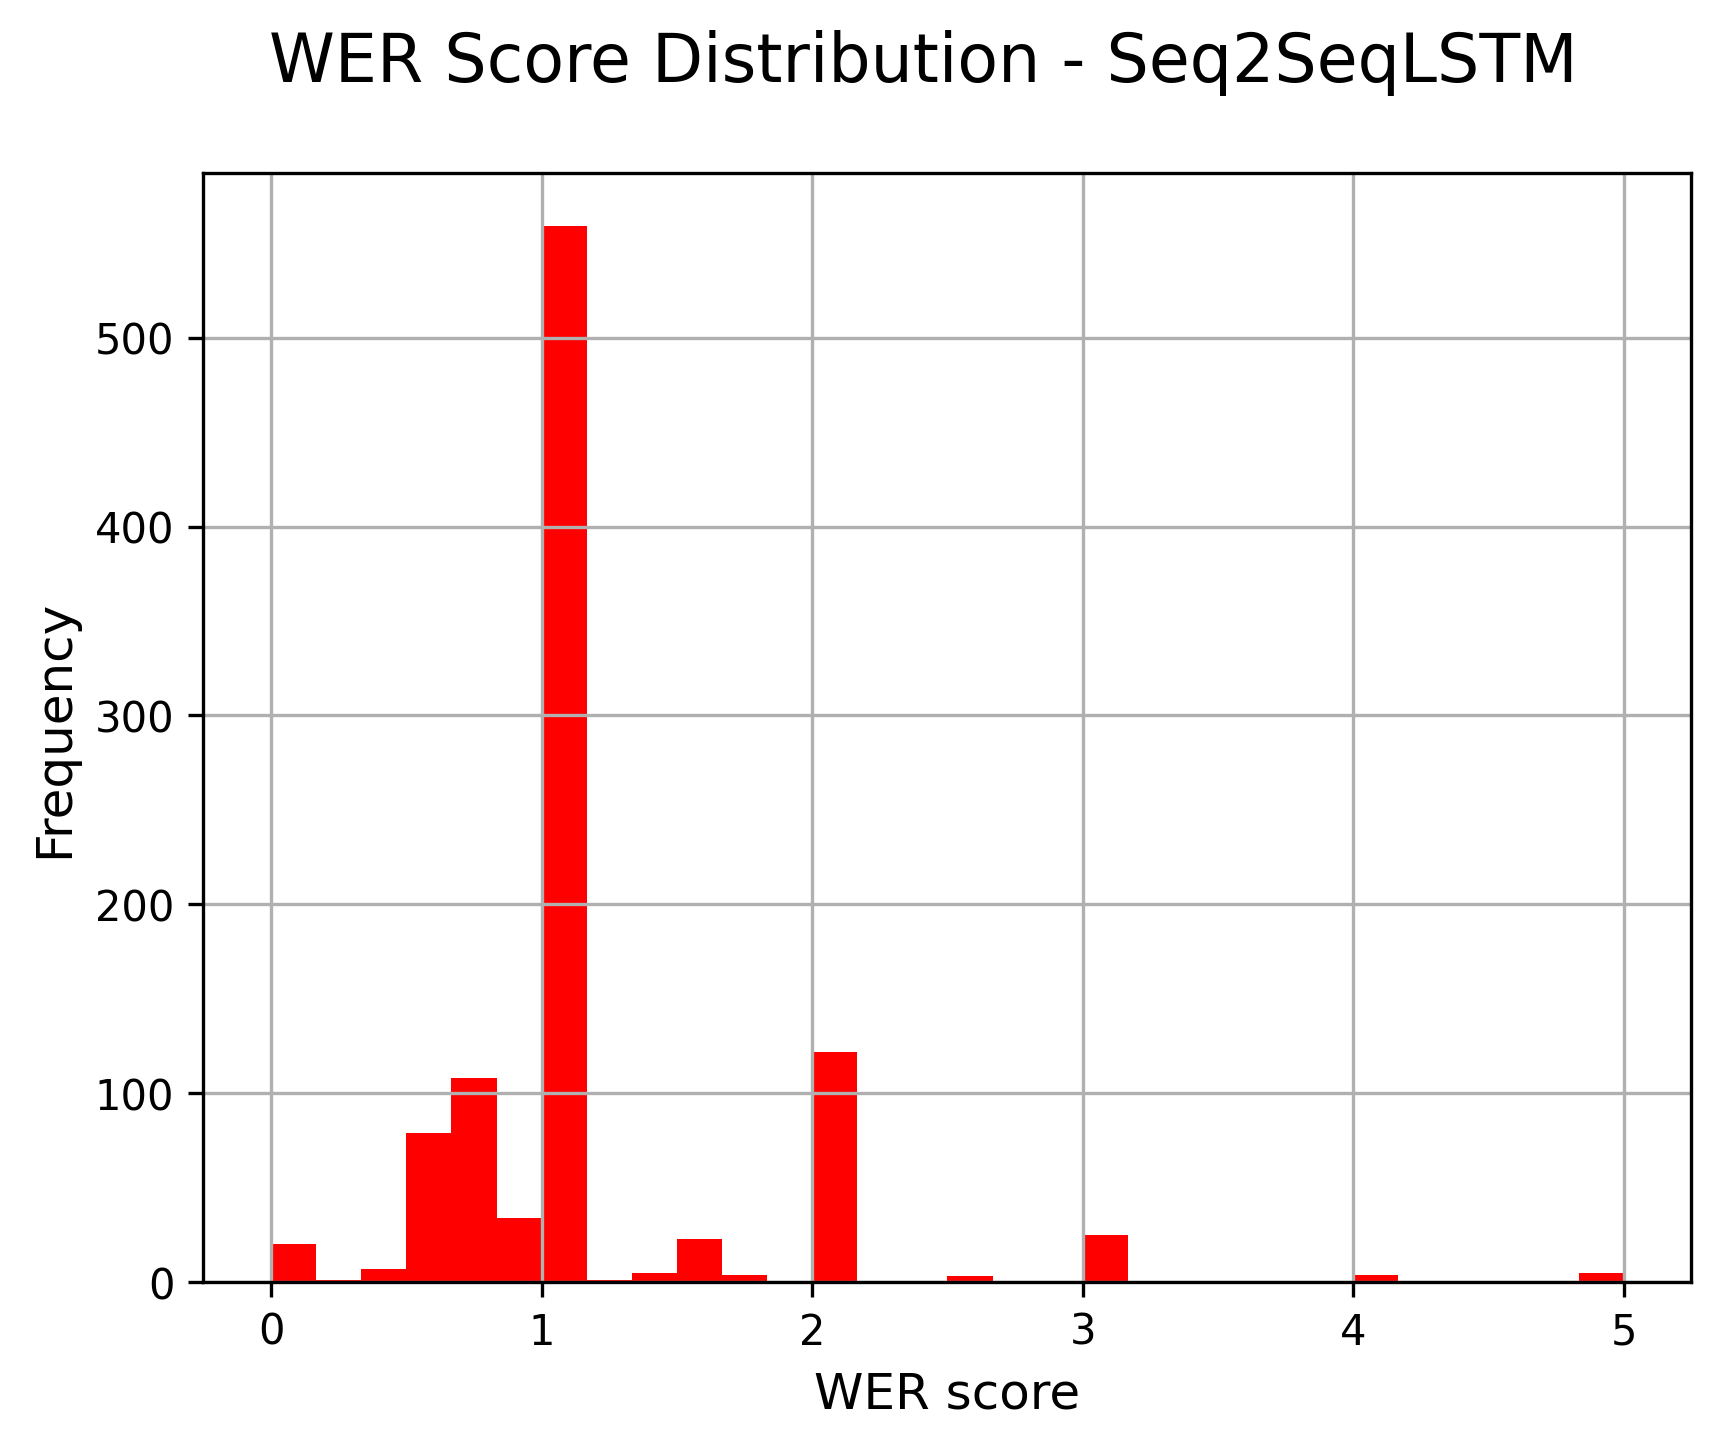
\includegraphics[width=\textwidth]{media/Seq2SeqLSTM_wer_scores.png}
        \caption{WER Seq2SeqLSTM}
    \end{subfigure}
    \hfill
    \begin{subfigure}{0.45\textwidth}
        \centering
        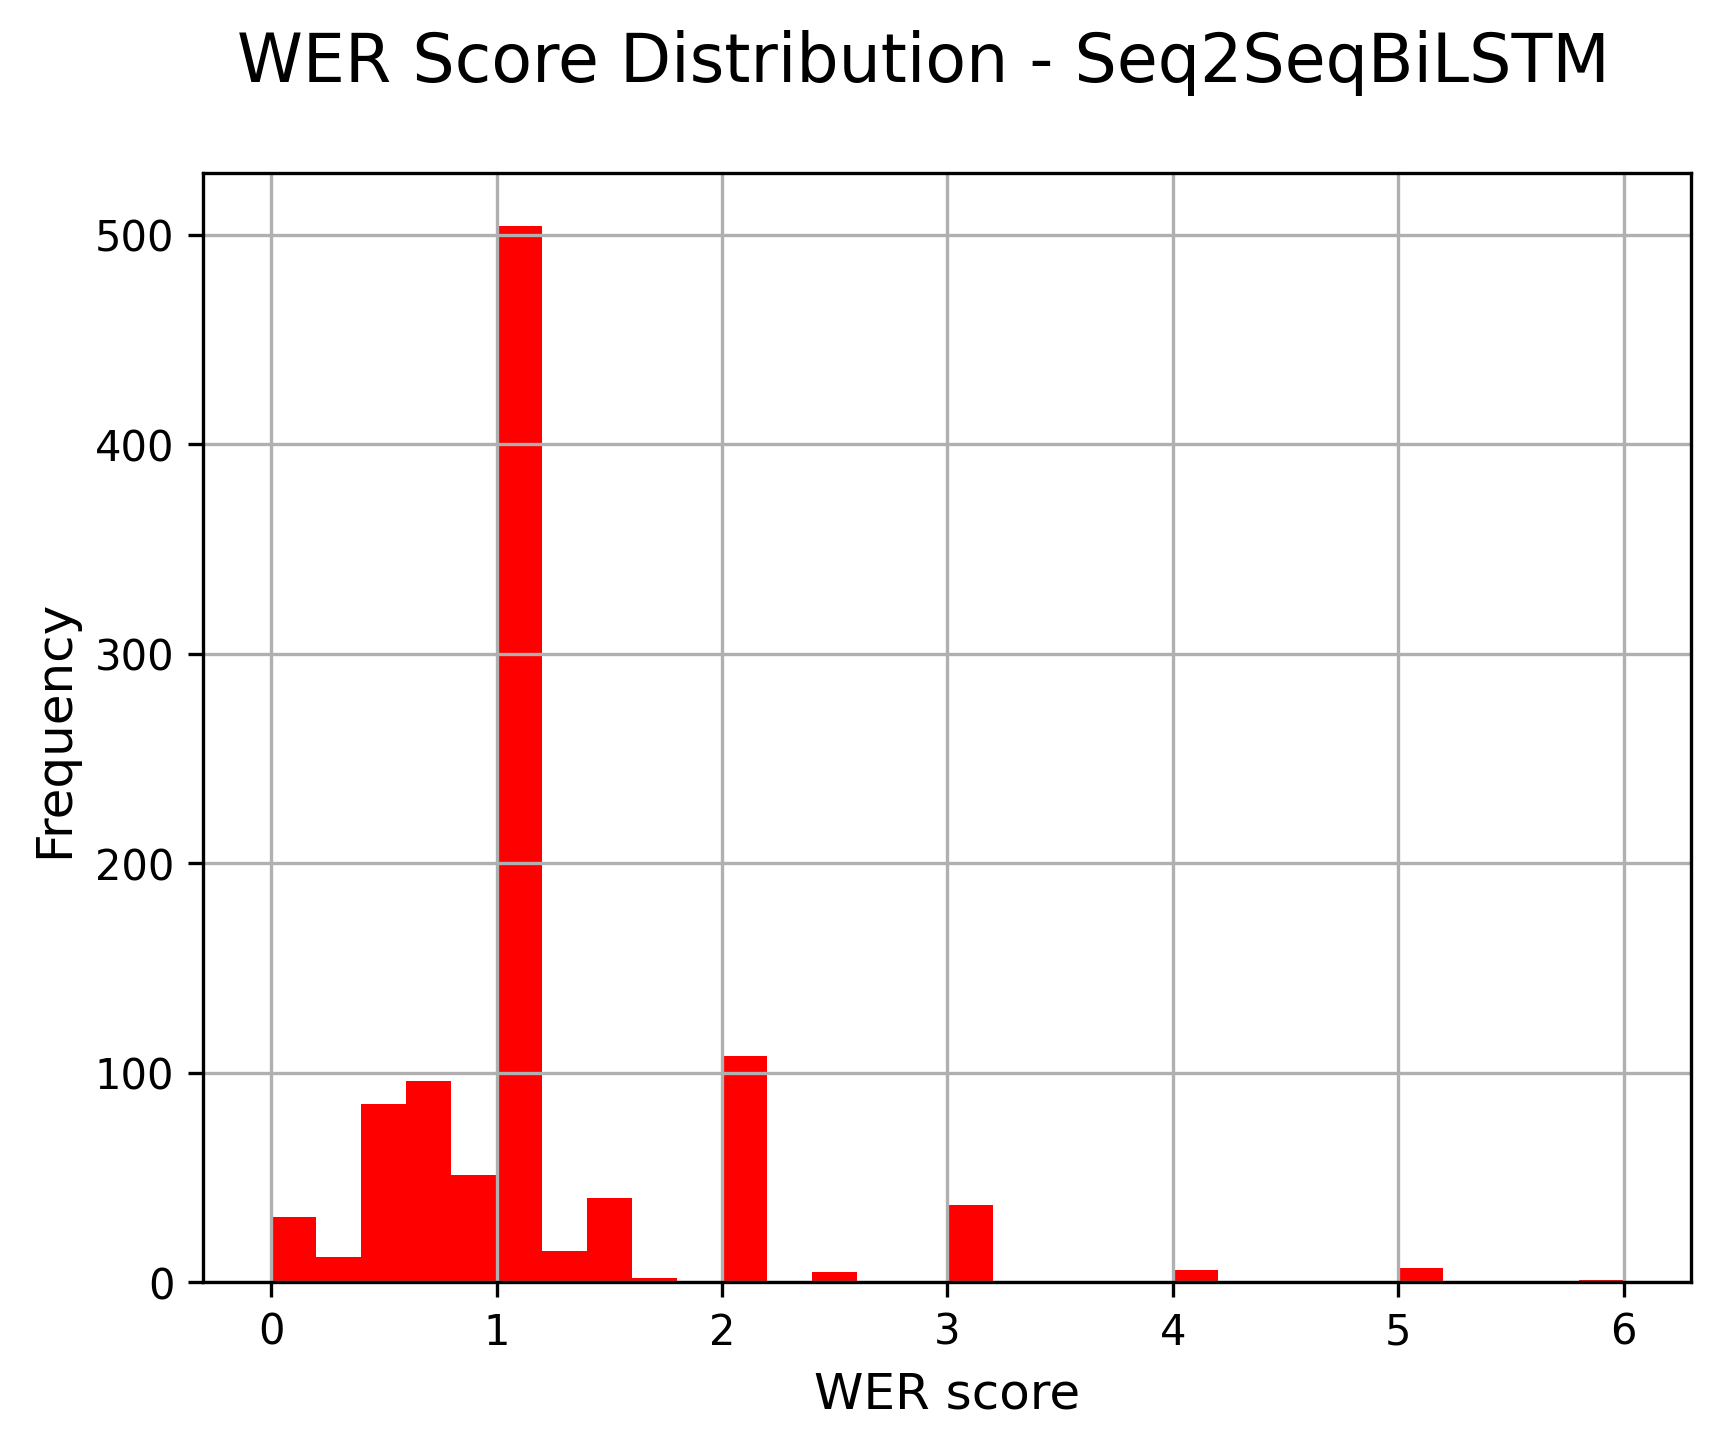
\includegraphics[width=\textwidth]{media/Seq2SeqBiLSTM_wer_scores.png}
        \caption{WER Seq2SeqBiLSTM}
    \end{subfigure}
    \caption{Confronto del Word Error Rate tra i modelli Seq2SeqLSTM e Seq2SeqBiLSTM.}
    \label{fig:wer_comparison}
\end{figure}

\subsection{Cosine Similarity}
La Figura \ref{fig:cosine_similarity_comparison} confronta i valori di similarità cosenica. Anche in questo caso, il modello Seq2SeqBiLSTM ottiene valori più alti, suggerendo una maggiore correlazione semantica con i riassunti di riferimento.

\begin{figure}[H]
    \centering
    \begin{subfigure}{0.45\textwidth}
        \centering
        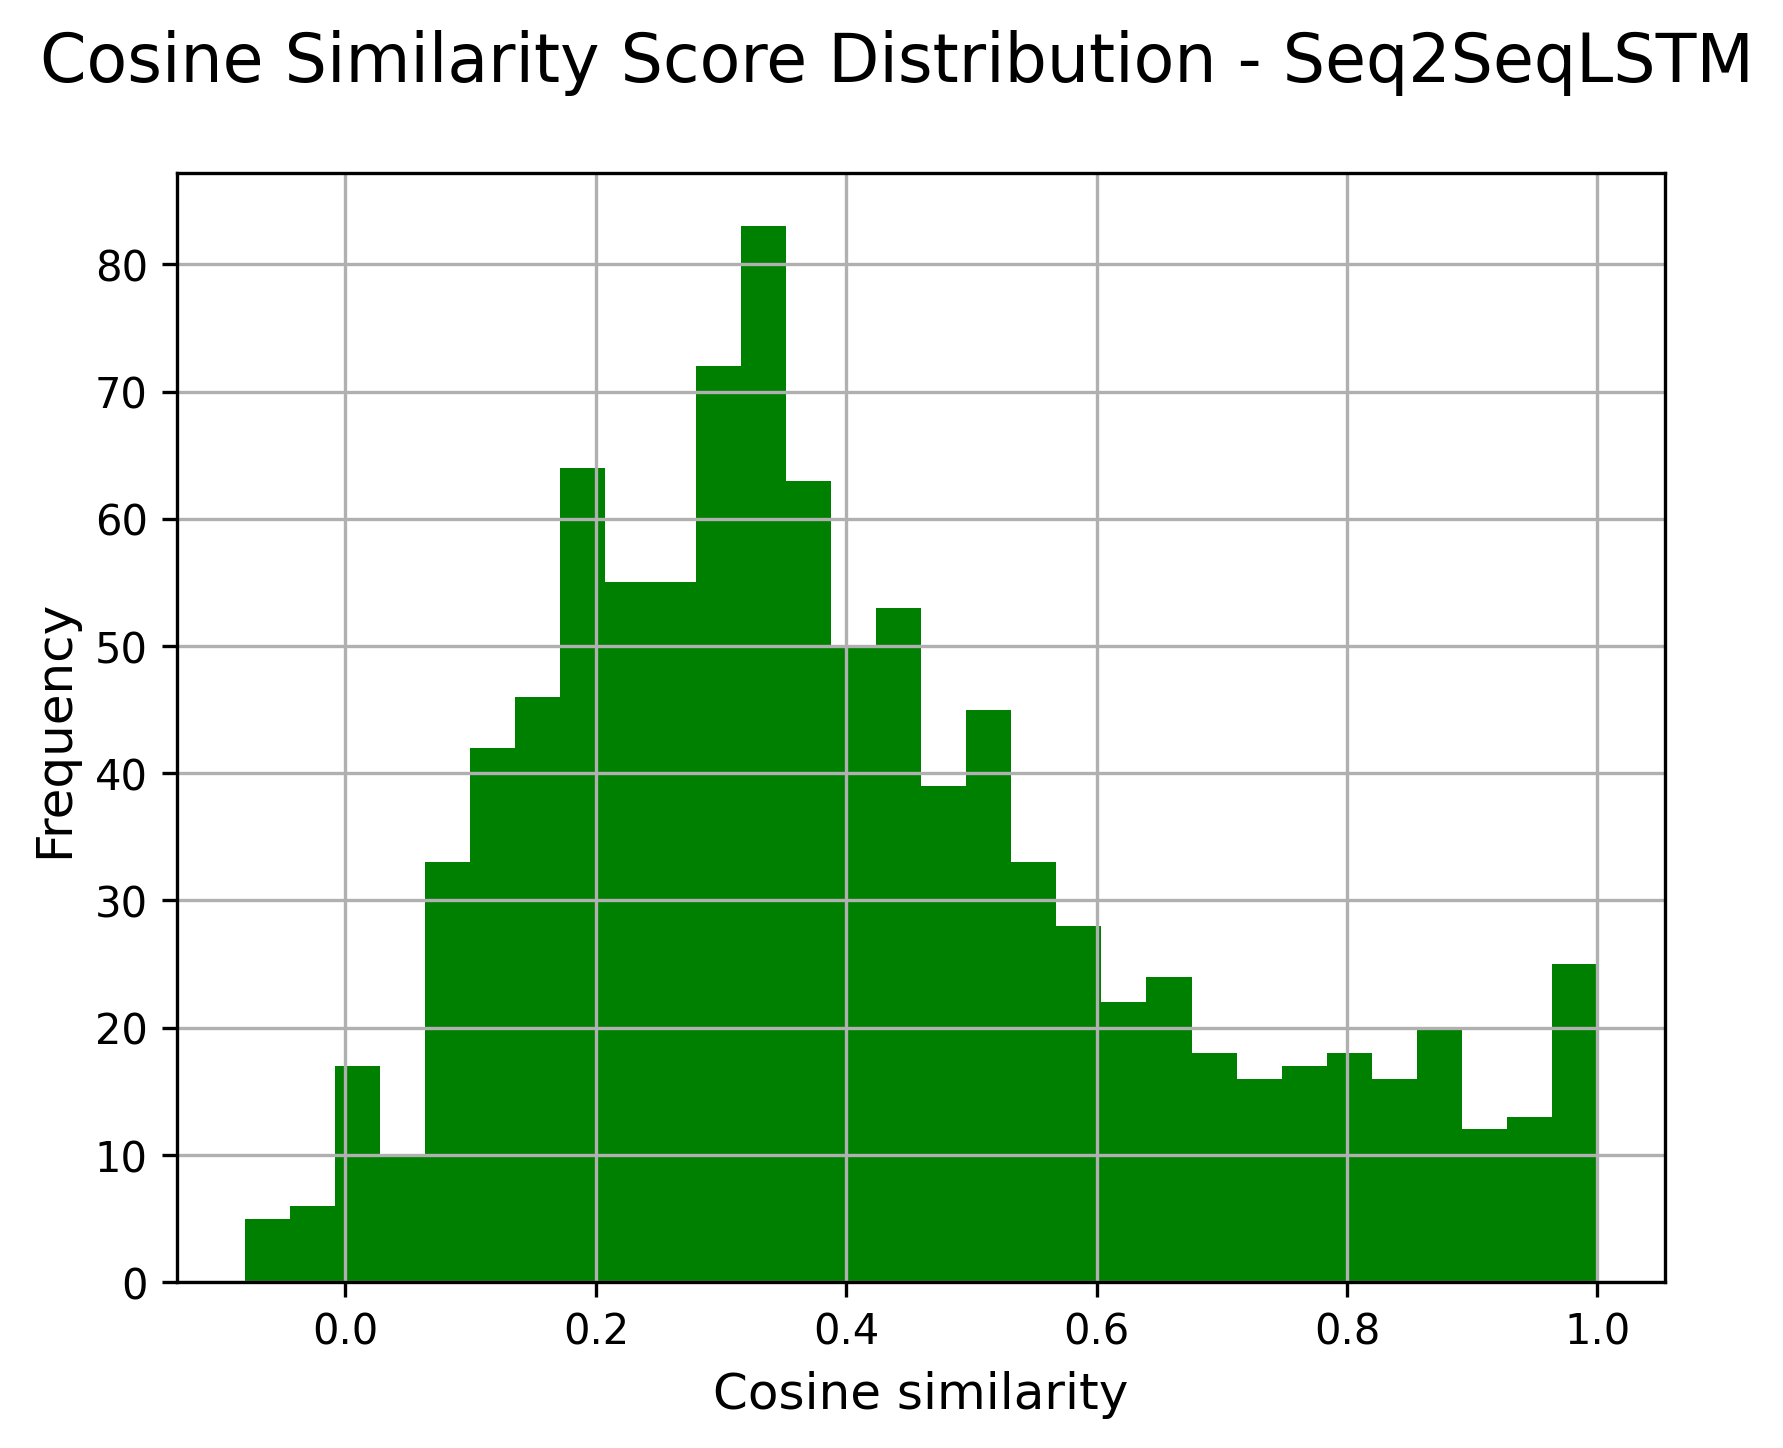
\includegraphics[width=\textwidth]{media/Seq2SeqLSTM_cosine_similarity_scores.png}
        \caption{Cosine Similarity Seq2SeqLSTM}
    \end{subfigure}
    \hfill
    \begin{subfigure}{0.45\textwidth}
        \centering
        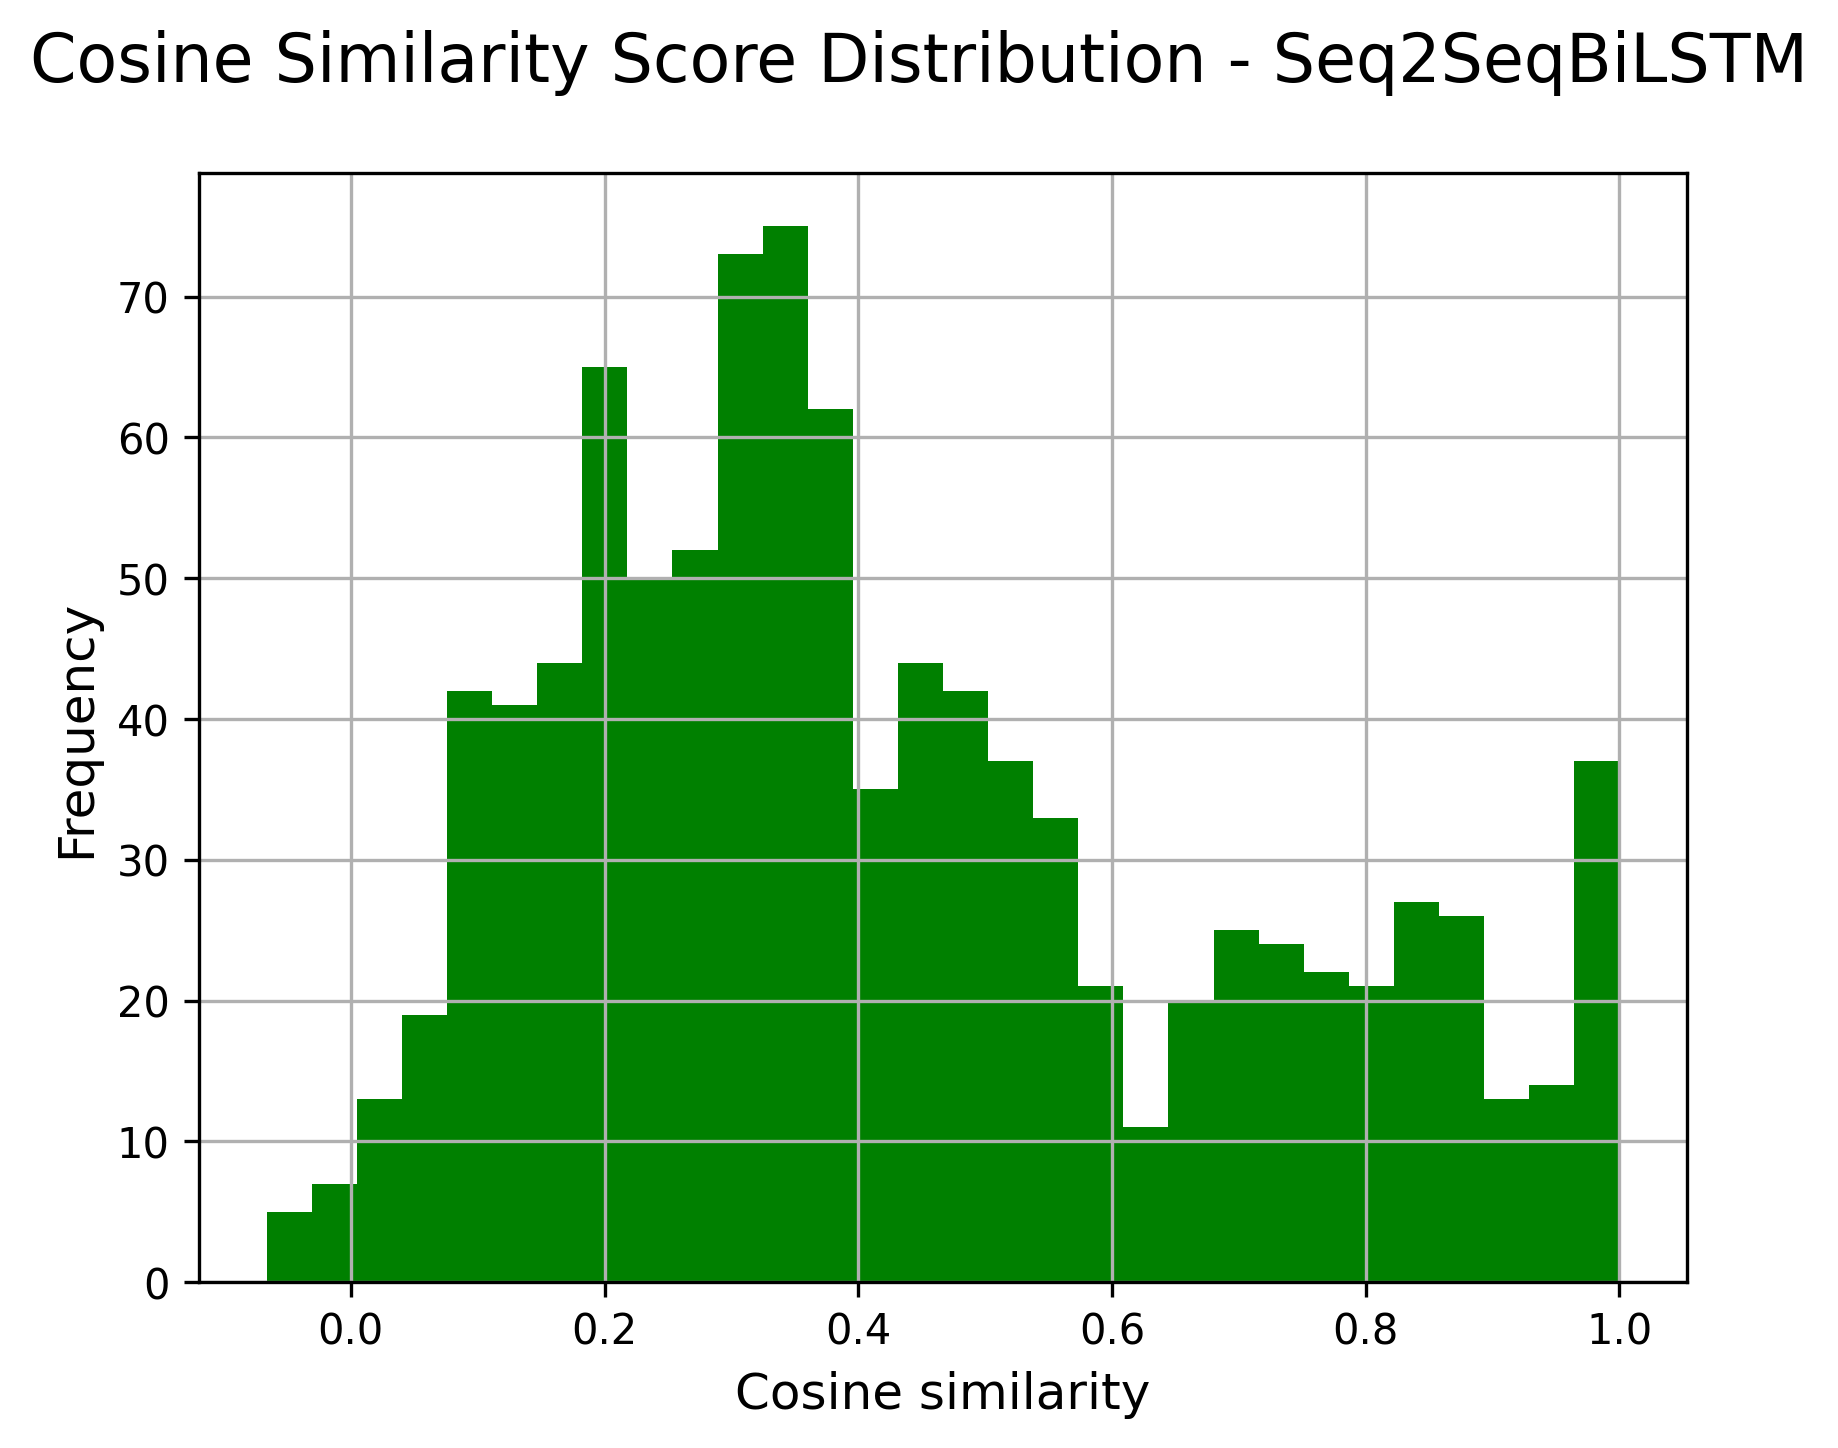
\includegraphics[width=\textwidth]{media/Seq2SeqBiLSTM_cosine_similarity_scores.png}
        \caption{Cosine Similarity Seq2SeqBiLSTM}
    \end{subfigure}
    \caption{Confronto della cosine similarity tra i modelli Seq2SeqLSTM e Seq2SeqBiLSTM.}
    \label{fig:cosine_similarity_comparison}
\end{figure}


\section{Conclusioni}
Il modello implementato dimostra la capacità di generare riassunti efficaci delle recensioni di prodotti.\\
I risultati complessivi indicano che il modello Seq2Seq LSTM ha difficoltà significative nel generare output precisi, sia dal punto di vista lessicale che sintattico. \\
Tuttavia, la similarità cosenica superiore a zero per la maggior parte delle righe suggerisce che il modello riesce a mantenere una correlazione semantica, seppure debole, con il testo di riferimento.\\
Per un fine di generazione di riassunti ci si può ritenere soddisfatti, grazie alla similarità cosenica.

\end{document}